%\documentclass[unicode,master]{scutthesis} % 草稿封面,硕士则添加选项master,博士则去掉。使用正式封面时注释该行
\documentclass[unicode,master,pdfcover]{scutthesis} %   % 论文正式封面,pdfcover为可选项,终稿再添加,使用草稿封面时注释该行
\usepackage{fontspec,color,array,longtable,graphicx} 
%%%%%%%%%%%%%%%%%%%%%%%%%%%%%%%%%%%%%%%%%%%%%%%%%%%%%%%%%%%%%%%%%%%%%%%%%%%%%%%%%%——by MCH
%编译范围
%\includeonly{chapter03}
%参考文献设置
\usepackage[backend=biber,style=gb7714-2015,gbalign=gb7714-2015,gbpub=false,gbnamefmt = lowercase]{biblatex}
\addbibresource[location=local]{MyLibrary.bib} % 如果在其他盘,改为相对路径。比如F盘,改为:F/MyLibrary.bib
\addbibresource[location=local]{mybibfile2.bib} % 无论什么来源的bib文件,只要由参考文献的BibTeX组成,都可以使用此模板。参考文献的BibTeX获取方法可百度
%页眉页脚设置
\usepackage{fancyhdr}
\usepackage{listings}
\usepackage{xunicode}
\renewcommand{\lstlistingname}{列表}
\pagestyle{fancy}
\fancyfoot[C]{\headfont\thepage}
\renewcommand{\chaptermark}[1]{\markboth{\chaptername\ #1}{}}
\renewcommand{\sectionmark}[1]{\markright{\thesection\ #1}}
\fancyhead[RE]{}
\fancyhead[RO]{}
\fancyhead[LE]{}
\fancyhead[LO]{}
\fancyhead[CO]{\headfont{\leftmark}}
\fancyhead[CE]{\headfont{华南理工大学硕士学位论文}}% 
\renewcommand{\headrulewidth}{1.5pt}
\renewcommand{\footrulewidth}{0pt}
%%%%%%%%%%%%%%%%%%%%%%%%%%%%%%%%%%%%%%%%%%%%%%%%%%%%%%%%%%%%%%%%%%%%%%%%%%%%%%%%%%
\usepackage[unicode=true,bookmarks=true,bookmarksnumbered=true,bookmarksopen=false,breaklinks=false,pdfborder={0 0 1},backref=false,colorlinks=true]{hyperref}
\hypersetup{pdftitle={LaTeX模板使用说明},
	pdfauthor={蒙超恒},
	pdfsubject={华南理工大学硕士学位论文},
%%	pdfsubject={华南理工大学博士学位论文},
	pdfkeywords={\LaTeX{};\LaTeX{}},
%%		linkcolor=black, anchorcolor=black, citecolor=black, filecolor=black, menucolor=black, urlcolor=black, pdfstartview=FitH}% 黑白,提交版
	linkcolor=blue, anchorcolor=black, citecolor=red, filecolor=magenta, menucolor=red, urlcolor=magenta, pdfstartview=FitH}% 彩色

\makeatletter
%%%%%%%%%%%%%%%%%%%%%%%%%%%%%% LyX specific LaTeX commands.
\providecommand{\LyX}{\texorpdfstring%
	{L\kern-.1667em\lower.25em\hbox{Y}\kern-.125emX\@}
	{LyX}}
%% Because html converters don't know tabularnewline
\providecommand{\tabularnewline}{\\}
\makeatother
\begin{document}
	%%%%%%%%%%%%%草稿封面设置%%%%%%%%%%%%%使用“正式封面”时不需要理会这部分
	\title{LaTeX模板使用说明}	
	\author{蒙超恒}	
	\supervisor{指导教师:裴海龙\ 教授}	
	\institute{华南理工大学}	
	\date{2020年5月20日}
	%%%%%%%%%%%%%%%%%%%%%%%%%%%%%%%%%%%%%
	\maketitle	
	\frontmatter	%此后为罗马数字页码,页面类型为plain
	\chapter{摘\texorpdfstring{\quad}{}要}
	本模板由Shun Xu\cite{_}以及yecfly\cite{_a}的模板修改而来,适合于华南理工大学硕/博士毕业论文。既然已经入坑LaTeX,就不推荐使用LYX,但本模板在修改祖传代码过程中仅对修改部分进行更新,其余部分仍保留源代码。另外参考文献管理软件推荐使用zotero,这也是本模板使用的软件。本模板最主要的改动是参考文献使用biber,而不是原来的bibtex,因此不再需要.bst文件。

\keywordsCN{\LaTeX{};论文}

\chapter{Abstract}
	

\keywordsEN{\LaTeX{}; Paper} % 中英文摘要
	%%%%%%%%%%%%%%%%%%%%%%%%%%%%%%%%%%%%%%%%%%%%%%%%
	% 目录、表格目录、插图目录这几个字本身的大纲级别是一级的,即和章名有相同的字号字体。目录表的内容通过titletoc宏包在。cls文件设置了。
	\tableofcontents	%目录
	\listoftables	%表格目录(可选)
	\listoffigures	%插图目录(可选)
	%%%%%%%%%%%%%%%%%%%%%%%%%%%%%%%%%%%%%%%%%%%%%%%%%
	\chapter{主要符号对照表}
【本节论文规范为可选,如果你的论文没有相关内容那么去除这一节;如果有,则删除这一行注释。】
\begin{table}
	\centering{}%
	\begin{tabular}{l>{\centering}p{0.5cm}l}
	 $ \bm{X}_n\bm{Y}_n\bm{Z}_n $-地理坐标系           &  & ${\bm{X}_b}{\bm{Y}_b}{\bm{Z}_b}$-机体坐标系\tabularnewline
	 $ \psi $-偏航角								   &  & $\theta$-俯仰角\tabularnewline
	 $\varphi$-滚转角  							   &  & $\bm{R}^n_b$、$\bm{R}$-机体系到NED系的旋转矩阵\tabularnewline
	 $\bm{G}$-NED系的重力  							  &  &   $\varphi_0 $-气动面安装角\tabularnewline
	 $ w $-系统的外部扰动								&  &  $T$-系统采样周期\tabularnewline
	 $\bm{F}$-机体系的气动力 						    &  &   $\bm{M}$-机体系的气动力矩\tabularnewline
	 $\rho$-空气密度 								  &  &  $C_{D,x} $、$ C_{D,y} $、$ C_{D,z} $-沿机体轴阻力系数\tabularnewline
	 $A_x $、$ A_y $、$ A_z $-沿机体轴的截面面积 		 &  &  $v$-机身相对于空气的速度分量\tabularnewline 
	 $l_{a}$-机身气动阻力作用点与重心的距离   			  &  &  $V_c$-气体在无穷远处的速度\tabularnewline
	 $T_d$-涵道体升力  								 &  &  $T_p$-风扇升力\tabularnewline
	 $T_a$-总升力 								      &  &  $q_a$-涵道升力分配系数\tabularnewline
	 $ p_U $-桨盘上表面压强 						   &  &  $p_L$-桨盘下表面压强\tabularnewline
	 $V_c+V_i$-桨盘上下表面气体速度 					 &  &  $S$-桨盘面积\tabularnewline
	 $ V_i $-桨盘处气流诱导速度 						  &  &  $ V_{cr} $-理想自转下降速率\tabularnewline
	 $ Q $-风扇扭矩 								 &  &  $ \varpi $-风扇转速\tabularnewline
	 $\mu$-环绕涵道角度变量 						  &  &  $\hat{\bm{i}}$-沿机体系$x$轴方向的单位矢量\tabularnewline 
	 $\hat{\bm{j}}$-沿机体系$y$轴方向的单位矢量  	   &  &  $C_{l, d}(\alpha_d)$-涵道翼型升力曲线\tabularnewline 
	 $C_{d, d}(\alpha_d)$涵道翼型阻力曲线  		      &  &  $c_d$-涵道翼型弦长\tabularnewline 
	 $C_{l_{\alpha}}$-风管翼型升力曲线斜率  			 &  &  $C_{l, \min }$、$ C_{l, \max } $-升力系数极限\tabularnewline 
	 $C_{d, o }$、$C_{d, g }$-拟合阻力曲线经验常数 	&  &  $R$-风扇半径\tabularnewline 
	 $C_{d u c t}$ - 常值比例系数  					&  &  $l_{d}$-重心与涵道气动力作用点的距离\tabularnewline
	 $k_{\delta}$-操纵面气动升力系数 				 &  &  $\alpha_d$-攻角\tabularnewline
	 $ I_{b}$-风扇转动惯量  						   &  &  $ d_{af} $ 、$ d_{ds} $-风扇扭矩常系数\tabularnewline
	 $\bm{L}_{{r}}$-风扇角动量  						&  & \tabularnewline 					
	\end{tabular}
\end{table}	% 符号对照表(可选)
	\chapter{英文缩略词}
【本节论文规范为可选,如果你的论文没有相关内容那么去除这一节;如果有,则删除这一行注释。】
\begin{table}
	\centering{}%
	\begin{tabular}{ccc}
		SCUT  & South China University of Technology & 华南理工大学\tabularnewline
		&  & \tabularnewline
		&  & \tabularnewline
		&  & \tabularnewline
		&  & \tabularnewline
	\end{tabular}
\end{table} 	% 缩略词	
	
	\mainmatter %此后为阿拉伯数字页码
	
    %%%%%%%%%%%%%%%%%%%%%%%%%%%%%%%%%%%%%%%%%%%%%%页眉页脚设置 ——by MCH 
    \fancypagestyle{plain}{
    	\pagestyle{fancy}
    }	% 每章的第一页会默认使用plain,没有页眉。通过重定义plain为fancy解决
    \pagestyle{fancy}	%设置页眉页脚为fancy
    %%%%%%%%%%%%%%%%%%%%%%%%%%%%%%%%%%%%%%%%%%%%%%分章节,结合导言区的\includeonly命令可仅编译部分章节,编译时不用切换界面,直接在相应章节编译即可。
	\chapter{绪论}
%
\section{研究背景和意义}
\subsection{研究背景和意义}
%
关于\LaTeX{}以及基于\LaTeX{}写作的好处不再赘述。\LaTeX{}的入门资料推荐文献\parencite{_g}以及文献\parencite{_c}。

这里主要是想推荐一种“学术生态”,即利用各种工具展开科研工作,以达到事半功倍的效果。需要用到以下软件:
\begin{enumerate}
	\item 	参考文献管理软件zotero\cite{_m}。很多人使用过endnote,但其实zotero也非常强大,强烈推荐。可到b站观看Struggle with Me出品的视频教程\cite{_k}入门。zotero不自带pdf阅读器,使用Adobe Acrobat pro DC即可。在Adobe中点击文件->属性->位置,即可打开文件所在位置,故亦不推荐更改zotero的文件系统。
	\item	可截图获取文献中公式的软件mathpix\cite{_h}。在阅读别人的论文时,很可能需要把文章中的公式抄下来放到自己的笔记中,方便以后组会报告甚至论文中使用,这时使用mathpix可直接截图获取\LaTeX{}源码,非常方便。该软件普通邮箱注册可每月50次免费,学校邮箱可100次,若信用卡注册可1000次。	
	\item	TeXstudio,相当于IDE。本模板是基于TeXstudio2020进行的,关于该软件的使用(快捷键等)可另行查找资料。编译时可以使用该软件,也可以运行文件目录的all.bat。TeXstudio的设置见第二章。
\end{enumerate}

本文的章节安排如下:

第一章,绪论。

第二章,模板简介。主要介绍各文件的内容。

第三章,常用环境。介绍论文写作中常用的环境,包括:图、表、公式、定理。基本涵盖了常用的命令。

%第三章,参考文献设置。本模板对旧版的改动主要是参考文献部分,本章将简单参考文献设置以及
%编译选项的设置等等。


%第一章
	\chapter{模板简介}
%
与很多外文杂志社不同,大部分中文期刊都不提供\LaTeX{}模板给投稿者使用,也很少有学校给学生提供官方的毕业论文模板。目前github上的大部分模板都是由学生发起的非官方模板。在此感谢Shun Xu以及yecfly等人的工作,他们的无私贡献使得华南理工大学硕博士毕业论文也可以使用\LaTeX{}撰写。

本模板是直接修改前人的模板得到的,更详细的介绍可到\parencite{_,_a}下载。本章仅从用户的角度简要介绍模板的使用,而尽量避免涉及\LaTeX{}的模板制作细节(实际上是因为本人也不会)。正如我们使用手机并不需要了解麦克斯韦方程组,使用\LaTeX{}写作也无需了解模板是如何制作的。

\LaTeX{}的源代码保存在后缀名为.tex的文件中。当编写长篇文档时,例如当编写书籍、毕业论文时,单个源文件会使修改、校对变得十分困
难。将源文件分割成若干个文件,例如将每章内容单独写在一个文件中,会大大简化修改和校对
的工作。为方便,本文将scutthesis.tex文件称为主文件,而将abstract.tex、chapter0x.tex、conclusion.tex等文件称为章节文件。

值得注意的是,要每次编译时都更新参考文献著录,TeXstudio软件的选项->设置中的构建并查看、编译器需要设置成如图\ref{TeXstudio}、\ref{setup}所示。此时只需在任意一个文件中点击构建并查看按钮即可编译文档。每次编译都更新参考文献会使得编译时间很长。
\begin{figure}[htbp]
	\centering
	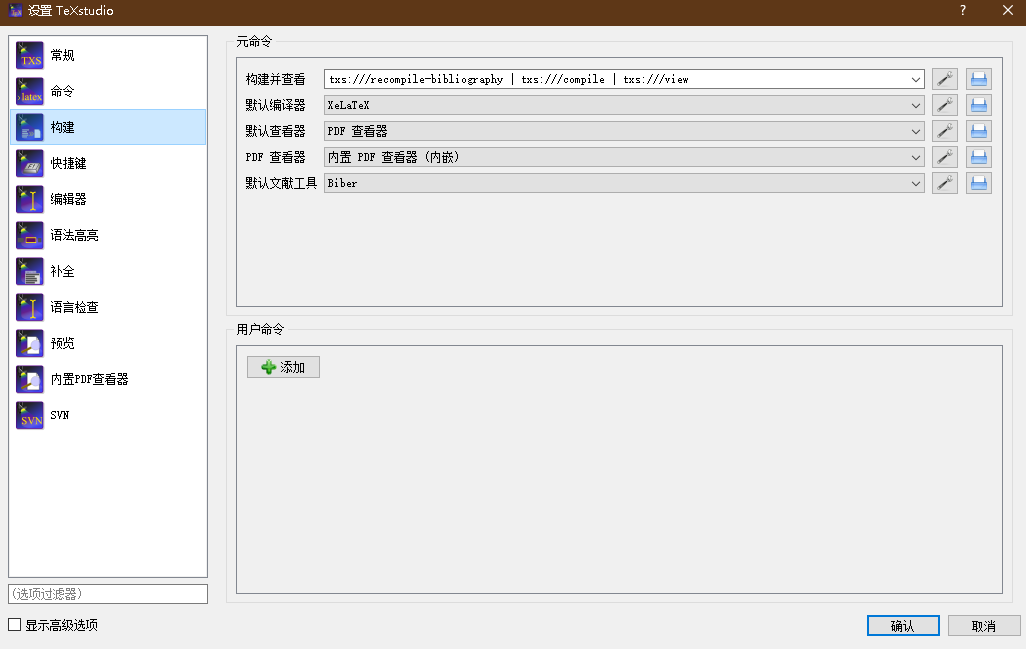
\includegraphics[scale=0.55]{Fig/TeXstudio.png}
	\caption{\label{TeXstudio}TeXstudio环境}
\end{figure}
\begin{figure}[htbp]
	\centering
	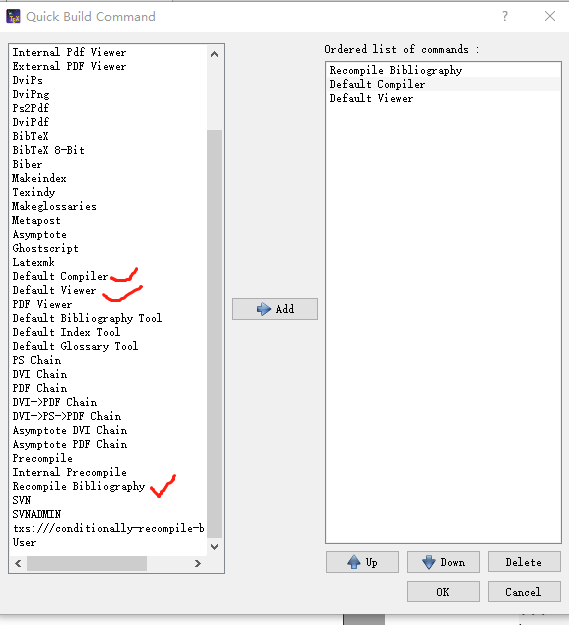
\includegraphics[scale=0.55]{Fig/setup.png}
	\caption{\label{setup}TeXstudio编译选项}
\end{figure}

\section{主文件}
scutthesis.tex文件相当于主函数,调用各章的内容。\LaTeX{}源代码以一个\textbackslash{}documentclass 命令作为开头,它指定了文档使用的文档类。文档类规定了\LaTeX{}源代码所要生成的文档的性质——普通文章、书籍、演示文稿、个人简
历等等。
\begin{lstlisting}
\documentclass[⟨options⟩]{⟨class-name⟩}
\end{lstlisting}
其中class-name为文档类的名称,如\LaTeX{}提供的article, book, report,可在其基础上派
生的一些文档类或者有其它功能的一些文档类。\LaTeX{}提供的基础文档类见文献\parencite{_c}。还可以自定义文档类,如华南理工大学硕博士论文文档类scutthesis,其实现保存在后缀名为.cls的文件中。可选参数options 为文档类指定选项。


document环境当中的内容是文档正文:
\begin{lstlisting}
\begin{document}
正文内容
\end{document}
\end{lstlisting}
正文中包含各章节内容:
\begin{lstlisting}
\chapter{摘\texorpdfstring{\quad}{}要}
	本模板由Shun Xu\cite{_}以及yecfly\cite{_a}的模板修改而来,适合于华南理工大学硕/博士毕业论文。既然已经入坑LaTeX,就不推荐使用LYX,但本模板在修改祖传代码过程中仅对修改部分进行更新,其余部分仍保留源代码。另外参考文献管理软件推荐使用zotero,这也是本模板使用的软件。本模板最主要的改动是参考文献使用biber,而不是原来的bibtex,因此不再需要.bst文件。

\keywordsCN{\LaTeX{};论文}

\chapter{Abstract}
	

\keywordsEN{\LaTeX{}; Paper} % 中英文摘要
\tableofcontents	% 目录
\listoftables	% 表格目录(可选)
\listoffigures	% 插图目录(可选)
\chapter{主要符号对照表}
【本节论文规范为可选,如果你的论文没有相关内容那么去除这一节;如果有,则删除这一行注释。】
\begin{table}
	\centering{}%
	\begin{tabular}{l>{\centering}p{0.5cm}l}
	 $ \bm{X}_n\bm{Y}_n\bm{Z}_n $-地理坐标系           &  & ${\bm{X}_b}{\bm{Y}_b}{\bm{Z}_b}$-机体坐标系\tabularnewline
	 $ \psi $-偏航角								   &  & $\theta$-俯仰角\tabularnewline
	 $\varphi$-滚转角  							   &  & $\bm{R}^n_b$、$\bm{R}$-机体系到NED系的旋转矩阵\tabularnewline
	 $\bm{G}$-NED系的重力  							  &  &   $\varphi_0 $-气动面安装角\tabularnewline
	 $ w $-系统的外部扰动								&  &  $T$-系统采样周期\tabularnewline
	 $\bm{F}$-机体系的气动力 						    &  &   $\bm{M}$-机体系的气动力矩\tabularnewline
	 $\rho$-空气密度 								  &  &  $C_{D,x} $、$ C_{D,y} $、$ C_{D,z} $-沿机体轴阻力系数\tabularnewline
	 $A_x $、$ A_y $、$ A_z $-沿机体轴的截面面积 		 &  &  $v$-机身相对于空气的速度分量\tabularnewline 
	 $l_{a}$-机身气动阻力作用点与重心的距离   			  &  &  $V_c$-气体在无穷远处的速度\tabularnewline
	 $T_d$-涵道体升力  								 &  &  $T_p$-风扇升力\tabularnewline
	 $T_a$-总升力 								      &  &  $q_a$-涵道升力分配系数\tabularnewline
	 $ p_U $-桨盘上表面压强 						   &  &  $p_L$-桨盘下表面压强\tabularnewline
	 $V_c+V_i$-桨盘上下表面气体速度 					 &  &  $S$-桨盘面积\tabularnewline
	 $ V_i $-桨盘处气流诱导速度 						  &  &  $ V_{cr} $-理想自转下降速率\tabularnewline
	 $ Q $-风扇扭矩 								 &  &  $ \varpi $-风扇转速\tabularnewline
	 $\mu$-环绕涵道角度变量 						  &  &  $\hat{\bm{i}}$-沿机体系$x$轴方向的单位矢量\tabularnewline 
	 $\hat{\bm{j}}$-沿机体系$y$轴方向的单位矢量  	   &  &  $C_{l, d}(\alpha_d)$-涵道翼型升力曲线\tabularnewline 
	 $C_{d, d}(\alpha_d)$涵道翼型阻力曲线  		      &  &  $c_d$-涵道翼型弦长\tabularnewline 
	 $C_{l_{\alpha}}$-风管翼型升力曲线斜率  			 &  &  $C_{l, \min }$、$ C_{l, \max } $-升力系数极限\tabularnewline 
	 $C_{d, o }$、$C_{d, g }$-拟合阻力曲线经验常数 	&  &  $R$-风扇半径\tabularnewline 
	 $C_{d u c t}$ - 常值比例系数  					&  &  $l_{d}$-重心与涵道气动力作用点的距离\tabularnewline
	 $k_{\delta}$-操纵面气动升力系数 				 &  &  $\alpha_d$-攻角\tabularnewline
	 $ I_{b}$-风扇转动惯量  						   &  &  $ d_{af} $ 、$ d_{ds} $-风扇扭矩常系数\tabularnewline
	 $\bm{L}_{{r}}$-风扇角动量  						&  & \tabularnewline 					
	\end{tabular}
\end{table}	% 符号对照表(可选)
\chapter{英文缩略词}
【本节论文规范为可选,如果你的论文没有相关内容那么去除这一节;如果有,则删除这一行注释。】
\begin{table}
	\centering{}%
	\begin{tabular}{ccc}
		SCUT  & South China University of Technology & 华南理工大学\tabularnewline
		&  & \tabularnewline
		&  & \tabularnewline
		&  & \tabularnewline
		&  & \tabularnewline
	\end{tabular}
\end{table} 	% 缩略词	
...
\chapter{绪论}
%
\section{研究背景和意义}
\subsection{研究背景和意义}
%
关于\LaTeX{}以及基于\LaTeX{}写作的好处不再赘述。\LaTeX{}的入门资料推荐文献\parencite{_g}以及文献\parencite{_c}。

这里主要是想推荐一种“学术生态”,即利用各种工具展开科研工作,以达到事半功倍的效果。需要用到以下软件:
\begin{enumerate}
	\item 	参考文献管理软件zotero\cite{_m}。很多人使用过endnote,但其实zotero也非常强大,强烈推荐。可到b站观看Struggle with Me出品的视频教程\cite{_k}入门。zotero不自带pdf阅读器,使用Adobe Acrobat pro DC即可。在Adobe中点击文件->属性->位置,即可打开文件所在位置,故亦不推荐更改zotero的文件系统。
	\item	可截图获取文献中公式的软件mathpix\cite{_h}。在阅读别人的论文时,很可能需要把文章中的公式抄下来放到自己的笔记中,方便以后组会报告甚至论文中使用,这时使用mathpix可直接截图获取\LaTeX{}源码,非常方便。该软件普通邮箱注册可每月50次免费,学校邮箱可100次,若信用卡注册可1000次。	
	\item	TeXstudio,相当于IDE。本模板是基于TeXstudio2020进行的,关于该软件的使用(快捷键等)可另行查找资料。编译时可以使用该软件,也可以运行文件目录的all.bat。TeXstudio的设置见第二章。
\end{enumerate}

本文的章节安排如下:

第一章,绪论。

第二章,模板简介。主要介绍各文件的内容。

第三章,常用环境。介绍论文写作中常用的环境,包括:图、表、公式、定理。基本涵盖了常用的命令。

%第三章,参考文献设置。本模板对旧版的改动主要是参考文献部分,本章将简单参考文献设置以及
%编译选项的设置等等。


	% 第一章
\chapter{模板简介}
%
与很多外文杂志社不同,大部分中文期刊都不提供\LaTeX{}模板给投稿者使用,也很少有学校给学生提供官方的毕业论文模板。目前github上的大部分模板都是由学生发起的非官方模板。在此感谢Shun Xu以及yecfly等人的工作,他们的无私贡献使得华南理工大学硕博士毕业论文也可以使用\LaTeX{}撰写。

本模板是直接修改前人的模板得到的,更详细的介绍可到\parencite{_,_a}下载。本章仅从用户的角度简要介绍模板的使用,而尽量避免涉及\LaTeX{}的模板制作细节(实际上是因为本人也不会)。正如我们使用手机并不需要了解麦克斯韦方程组,使用\LaTeX{}写作也无需了解模板是如何制作的。

\LaTeX{}的源代码保存在后缀名为.tex的文件中。当编写长篇文档时,例如当编写书籍、毕业论文时,单个源文件会使修改、校对变得十分困
难。将源文件分割成若干个文件,例如将每章内容单独写在一个文件中,会大大简化修改和校对
的工作。为方便,本文将scutthesis.tex文件称为主文件,而将abstract.tex、chapter0x.tex、conclusion.tex等文件称为章节文件。

值得注意的是,要每次编译时都更新参考文献著录,TeXstudio软件的选项->设置中的构建并查看、编译器需要设置成如图\ref{TeXstudio}、\ref{setup}所示。此时只需在任意一个文件中点击构建并查看按钮即可编译文档。每次编译都更新参考文献会使得编译时间很长。
\begin{figure}[htbp]
	\centering
	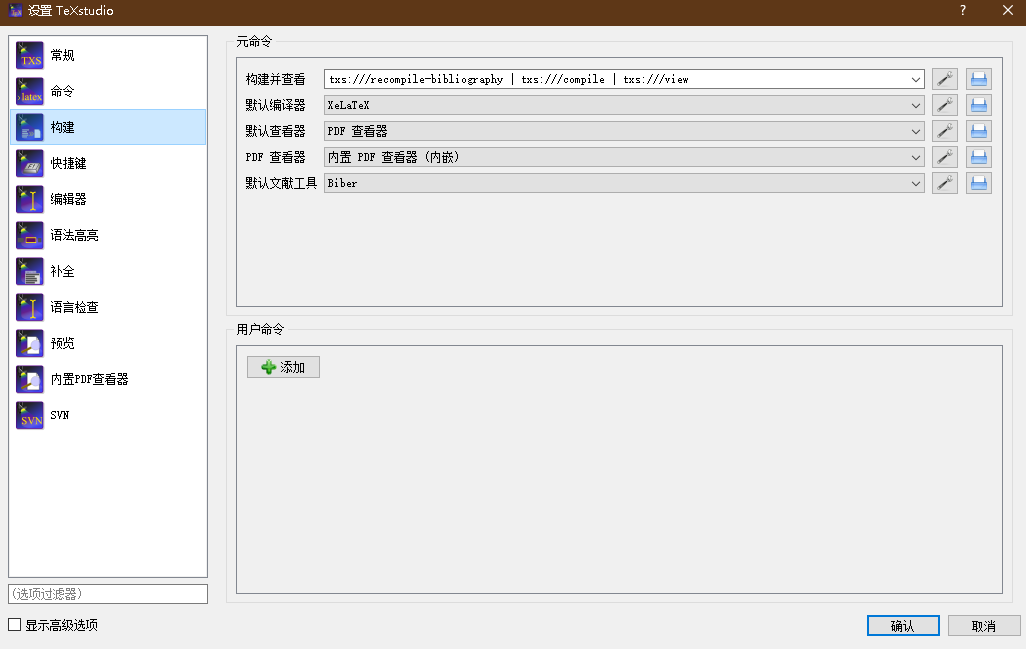
\includegraphics[scale=0.55]{Fig/TeXstudio.png}
	\caption{\label{TeXstudio}TeXstudio环境}
\end{figure}
\begin{figure}[htbp]
	\centering
	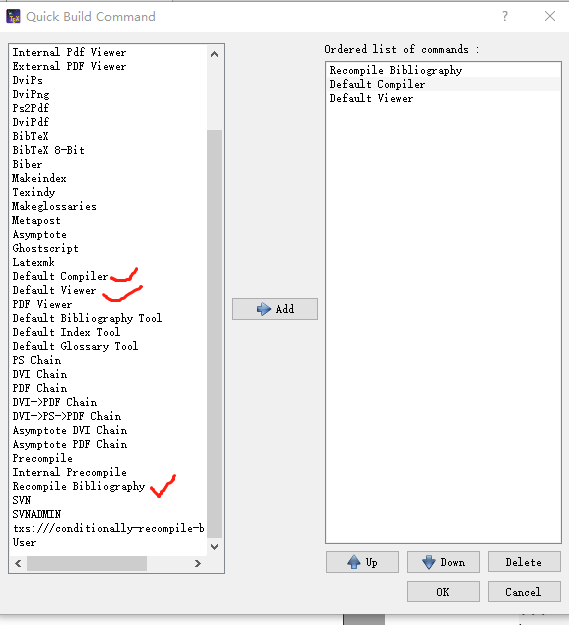
\includegraphics[scale=0.55]{Fig/setup.png}
	\caption{\label{setup}TeXstudio编译选项}
\end{figure}

\section{主文件}
scutthesis.tex文件相当于主函数,调用各章的内容。\LaTeX{}源代码以一个\textbackslash{}documentclass 命令作为开头,它指定了文档使用的文档类。文档类规定了\LaTeX{}源代码所要生成的文档的性质——普通文章、书籍、演示文稿、个人简
历等等。
\begin{lstlisting}
\documentclass[⟨options⟩]{⟨class-name⟩}
\end{lstlisting}
其中class-name为文档类的名称,如\LaTeX{}提供的article, book, report,可在其基础上派
生的一些文档类或者有其它功能的一些文档类。\LaTeX{}提供的基础文档类见文献\parencite{_c}。还可以自定义文档类,如华南理工大学硕博士论文文档类scutthesis,其实现保存在后缀名为.cls的文件中。可选参数options 为文档类指定选项。


document环境当中的内容是文档正文:
\begin{lstlisting}
\begin{document}
正文内容
\end{document}
\end{lstlisting}
正文中包含各章节内容:
\begin{lstlisting}
\chapter{摘\texorpdfstring{\quad}{}要}
	本模板由Shun Xu\cite{_}以及yecfly\cite{_a}的模板修改而来,适合于华南理工大学硕/博士毕业论文。既然已经入坑LaTeX,就不推荐使用LYX,但本模板在修改祖传代码过程中仅对修改部分进行更新,其余部分仍保留源代码。另外参考文献管理软件推荐使用zotero,这也是本模板使用的软件。本模板最主要的改动是参考文献使用biber,而不是原来的bibtex,因此不再需要.bst文件。

\keywordsCN{\LaTeX{};论文}

\chapter{Abstract}
	

\keywordsEN{\LaTeX{}; Paper} % 中英文摘要
\tableofcontents	% 目录
\listoftables	% 表格目录(可选)
\listoffigures	% 插图目录(可选)
\chapter{主要符号对照表}
【本节论文规范为可选,如果你的论文没有相关内容那么去除这一节;如果有,则删除这一行注释。】
\begin{table}
	\centering{}%
	\begin{tabular}{l>{\centering}p{0.5cm}l}
	 $ \bm{X}_n\bm{Y}_n\bm{Z}_n $-地理坐标系           &  & ${\bm{X}_b}{\bm{Y}_b}{\bm{Z}_b}$-机体坐标系\tabularnewline
	 $ \psi $-偏航角								   &  & $\theta$-俯仰角\tabularnewline
	 $\varphi$-滚转角  							   &  & $\bm{R}^n_b$、$\bm{R}$-机体系到NED系的旋转矩阵\tabularnewline
	 $\bm{G}$-NED系的重力  							  &  &   $\varphi_0 $-气动面安装角\tabularnewline
	 $ w $-系统的外部扰动								&  &  $T$-系统采样周期\tabularnewline
	 $\bm{F}$-机体系的气动力 						    &  &   $\bm{M}$-机体系的气动力矩\tabularnewline
	 $\rho$-空气密度 								  &  &  $C_{D,x} $、$ C_{D,y} $、$ C_{D,z} $-沿机体轴阻力系数\tabularnewline
	 $A_x $、$ A_y $、$ A_z $-沿机体轴的截面面积 		 &  &  $v$-机身相对于空气的速度分量\tabularnewline 
	 $l_{a}$-机身气动阻力作用点与重心的距离   			  &  &  $V_c$-气体在无穷远处的速度\tabularnewline
	 $T_d$-涵道体升力  								 &  &  $T_p$-风扇升力\tabularnewline
	 $T_a$-总升力 								      &  &  $q_a$-涵道升力分配系数\tabularnewline
	 $ p_U $-桨盘上表面压强 						   &  &  $p_L$-桨盘下表面压强\tabularnewline
	 $V_c+V_i$-桨盘上下表面气体速度 					 &  &  $S$-桨盘面积\tabularnewline
	 $ V_i $-桨盘处气流诱导速度 						  &  &  $ V_{cr} $-理想自转下降速率\tabularnewline
	 $ Q $-风扇扭矩 								 &  &  $ \varpi $-风扇转速\tabularnewline
	 $\mu$-环绕涵道角度变量 						  &  &  $\hat{\bm{i}}$-沿机体系$x$轴方向的单位矢量\tabularnewline 
	 $\hat{\bm{j}}$-沿机体系$y$轴方向的单位矢量  	   &  &  $C_{l, d}(\alpha_d)$-涵道翼型升力曲线\tabularnewline 
	 $C_{d, d}(\alpha_d)$涵道翼型阻力曲线  		      &  &  $c_d$-涵道翼型弦长\tabularnewline 
	 $C_{l_{\alpha}}$-风管翼型升力曲线斜率  			 &  &  $C_{l, \min }$、$ C_{l, \max } $-升力系数极限\tabularnewline 
	 $C_{d, o }$、$C_{d, g }$-拟合阻力曲线经验常数 	&  &  $R$-风扇半径\tabularnewline 
	 $C_{d u c t}$ - 常值比例系数  					&  &  $l_{d}$-重心与涵道气动力作用点的距离\tabularnewline
	 $k_{\delta}$-操纵面气动升力系数 				 &  &  $\alpha_d$-攻角\tabularnewline
	 $ I_{b}$-风扇转动惯量  						   &  &  $ d_{af} $ 、$ d_{ds} $-风扇扭矩常系数\tabularnewline
	 $\bm{L}_{{r}}$-风扇角动量  						&  & \tabularnewline 					
	\end{tabular}
\end{table}	% 符号对照表(可选)
\chapter{英文缩略词}
【本节论文规范为可选,如果你的论文没有相关内容那么去除这一节;如果有,则删除这一行注释。】
\begin{table}
	\centering{}%
	\begin{tabular}{ccc}
		SCUT  & South China University of Technology & 华南理工大学\tabularnewline
		&  & \tabularnewline
		&  & \tabularnewline
		&  & \tabularnewline
		&  & \tabularnewline
	\end{tabular}
\end{table} 	% 缩略词	
...
\chapter{绪论}
%
\section{研究背景和意义}
\subsection{研究背景和意义}
%
关于\LaTeX{}以及基于\LaTeX{}写作的好处不再赘述。\LaTeX{}的入门资料推荐文献\parencite{_g}以及文献\parencite{_c}。

这里主要是想推荐一种“学术生态”,即利用各种工具展开科研工作,以达到事半功倍的效果。需要用到以下软件:
\begin{enumerate}
	\item 	参考文献管理软件zotero\cite{_m}。很多人使用过endnote,但其实zotero也非常强大,强烈推荐。可到b站观看Struggle with Me出品的视频教程\cite{_k}入门。zotero不自带pdf阅读器,使用Adobe Acrobat pro DC即可。在Adobe中点击文件->属性->位置,即可打开文件所在位置,故亦不推荐更改zotero的文件系统。
	\item	可截图获取文献中公式的软件mathpix\cite{_h}。在阅读别人的论文时,很可能需要把文章中的公式抄下来放到自己的笔记中,方便以后组会报告甚至论文中使用,这时使用mathpix可直接截图获取\LaTeX{}源码,非常方便。该软件普通邮箱注册可每月50次免费,学校邮箱可100次,若信用卡注册可1000次。	
	\item	TeXstudio,相当于IDE。本模板是基于TeXstudio2020进行的,关于该软件的使用(快捷键等)可另行查找资料。编译时可以使用该软件,也可以运行文件目录的all.bat。TeXstudio的设置见第二章。
\end{enumerate}

本文的章节安排如下:

第一章,绪论。

第二章,模板简介。主要介绍各文件的内容。

第三章,常用环境。介绍论文写作中常用的环境,包括:图、表、公式、定理。基本涵盖了常用的命令。

%第三章,参考文献设置。本模板对旧版的改动主要是参考文献部分,本章将简单参考文献设置以及
%编译选项的设置等等。


	% 第一章
\chapter{模板简介}
%
与很多外文杂志社不同,大部分中文期刊都不提供\LaTeX{}模板给投稿者使用,也很少有学校给学生提供官方的毕业论文模板。目前github上的大部分模板都是由学生发起的非官方模板。在此感谢Shun Xu以及yecfly等人的工作,他们的无私贡献使得华南理工大学硕博士毕业论文也可以使用\LaTeX{}撰写。

本模板是直接修改前人的模板得到的,更详细的介绍可到\parencite{_,_a}下载。本章仅从用户的角度简要介绍模板的使用,而尽量避免涉及\LaTeX{}的模板制作细节(实际上是因为本人也不会)。正如我们使用手机并不需要了解麦克斯韦方程组,使用\LaTeX{}写作也无需了解模板是如何制作的。

\LaTeX{}的源代码保存在后缀名为.tex的文件中。当编写长篇文档时,例如当编写书籍、毕业论文时,单个源文件会使修改、校对变得十分困
难。将源文件分割成若干个文件,例如将每章内容单独写在一个文件中,会大大简化修改和校对
的工作。为方便,本文将scutthesis.tex文件称为主文件,而将abstract.tex、chapter0x.tex、conclusion.tex等文件称为章节文件。

值得注意的是,要每次编译时都更新参考文献著录,TeXstudio软件的选项->设置中的构建并查看、编译器需要设置成如图\ref{TeXstudio}、\ref{setup}所示。此时只需在任意一个文件中点击构建并查看按钮即可编译文档。每次编译都更新参考文献会使得编译时间很长。
\begin{figure}[htbp]
	\centering
	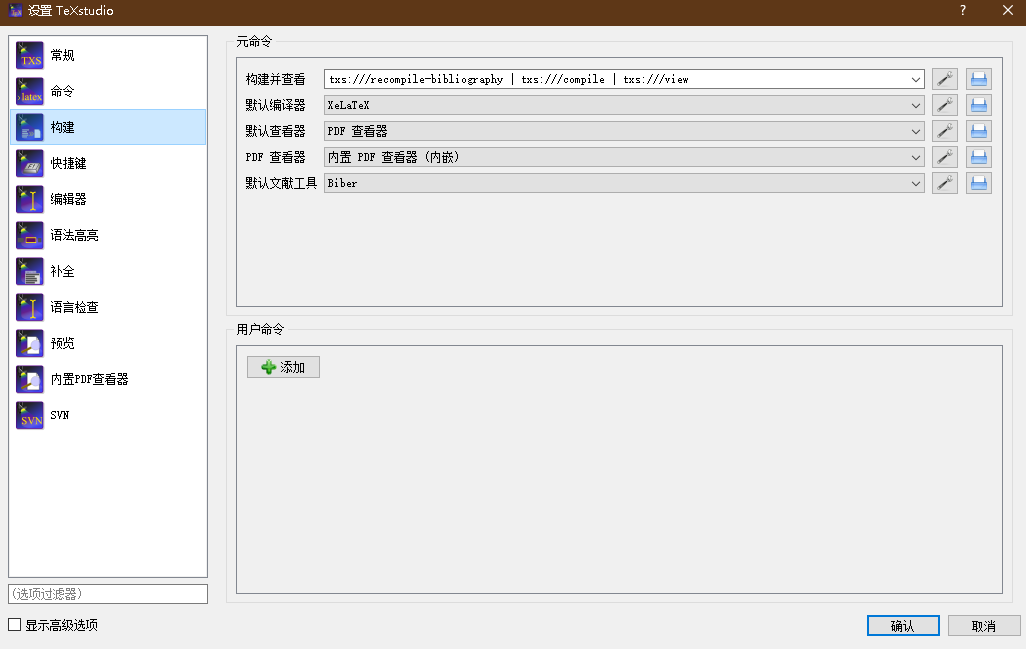
\includegraphics[scale=0.55]{Fig/TeXstudio.png}
	\caption{\label{TeXstudio}TeXstudio环境}
\end{figure}
\begin{figure}[htbp]
	\centering
	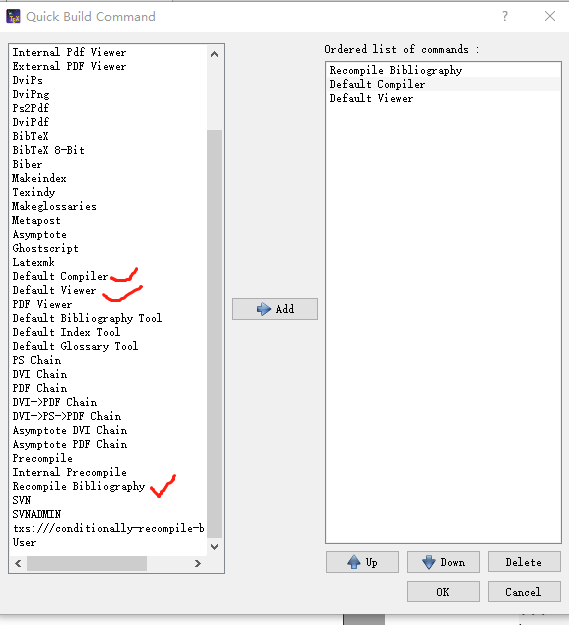
\includegraphics[scale=0.55]{Fig/setup.png}
	\caption{\label{setup}TeXstudio编译选项}
\end{figure}

\section{主文件}
scutthesis.tex文件相当于主函数,调用各章的内容。\LaTeX{}源代码以一个\textbackslash{}documentclass 命令作为开头,它指定了文档使用的文档类。文档类规定了\LaTeX{}源代码所要生成的文档的性质——普通文章、书籍、演示文稿、个人简
历等等。
\begin{lstlisting}
\documentclass[⟨options⟩]{⟨class-name⟩}
\end{lstlisting}
其中class-name为文档类的名称,如\LaTeX{}提供的article, book, report,可在其基础上派
生的一些文档类或者有其它功能的一些文档类。\LaTeX{}提供的基础文档类见文献\parencite{_c}。还可以自定义文档类,如华南理工大学硕博士论文文档类scutthesis,其实现保存在后缀名为.cls的文件中。可选参数options 为文档类指定选项。


document环境当中的内容是文档正文:
\begin{lstlisting}
\begin{document}
正文内容
\end{document}
\end{lstlisting}
正文中包含各章节内容:
\begin{lstlisting}
\include{abstract} % 中英文摘要
\tableofcontents	% 目录
\listoftables	% 表格目录(可选)
\listoffigures	% 插图目录(可选)
\include{symbols}	% 符号对照表(可选)
\include{abbreviation} 	% 缩略词	
...
\include{chapter01}	% 第一章
\include{chapter02} % 第二章
\include{chapter03} % 第三章
% 自行根据需要添加章节。
...
\include{conclusion} % 结论
...
\printbibliography	% 参考文献著录
\include{appendix} % 附录
\include{pub} % 成果
\include{ack} % 致谢
\end{lstlisting}
其中$\%$之后的内容为注释,...表示省略其他代码,仅保留论文内容主体部分。\textbackslash{}include\{xxx\}指令用于包含xxx.tex文件的内容,各章节的内容主要在xxx.tex中保存。在\textbackslash{}documentclass 和\textbackslash{}begin\{document\} 之间的位置称为导言区。在导言区中一般会使用\textbackslash{}usepackage 调用宏包,以及会进行对文档的全局设置。本模板的导言区除调用所需的宏包外,还进行了页眉页脚的设置。有的模板会把所有调用宏包的指令放到一个.sty宏包文件中,页面的设置放在文档类文件.cls文件中。因本人时间有限,就不做整理,欢迎有志之士加入完善。使用本模板并不需要了解导言区的指令,在需要时额外添加即可(要注意宏包冲突)。特别地,\textbackslash{}includeonly\{xxx\}指令用于使文档仅编译xxx.tex文件的内容,这就是分章节包含(include)的好处,可大大减少编译时间。

将封面打印保存为 thesis\_cover.pdf 文件,硕士使用master\_cover.docx ,博士使用 doctor\_cover.doc 。如果有更新版本的封面,可自行替换。文档类默认是博士论文,下面指令将控制添加封面与否:
\begin{lstlisting}
\documentclass[unicode,master,pdfcover]{scutthesis}	% 使用pdf文件封面的 硕士模板
\documentclass[unicode,master]{scutthesis}	% 不使用pdf文件封面的 硕士模板
\documentclass[unicode,pdfcover]{scutthesis}	% 使用pdf文件封面的博士模板
\documentclass[unicode]{scutthesis}	% 不使用pdf文件封面的博士模板
\end{lstlisting}
不使用thesis\_cover.pdf 文件指定的封面时,将使用草稿封面。草稿封面也可以减少编译时间,因此可以在最终提交论文时再使用论文封面。草稿封面用以下指令设置:
\begin{lstlisting}
%%%%%%%%%%%%%草稿封面设置%%%%%%%%%%%%%	
\title{LaTeX模板}	
\author{蒙超恒}	
\supervisor{指导教师:裴海龙\ 教授}	
\institute{华南理工大学}	
\date{2020年5月20日}
%%%%%%%%%%%%%%%%%%%%%%%%%%%%%%%%%%%%%
\end{lstlisting}
\section{章节文件}
章节文件如chapter0x.tex等,其内容由\textbackslash{}chapter\{章名\}开头。新建一章可新建一个文件并由\textbackslash{}chapter\{新建章名\}开头填写内容即可。节及小节分别用\textbackslash{}section\{新建节名\}、\textbackslash{}subsection\{新建小节名\}命令。

正文的的书写和txt文本文件的书写类似。\LaTeX{} 源代码中,空格键和Tab键输入的空白字符视为“空格”。连续的若干个空白字符视为一个空格。一行开头的空格忽略不计。行末的回车视为一个空格;但连续两个回车,也就是空行,会将文字分段。多个空行被视为一个空行。也可以在行末使用\textbackslash{}par 命令分段。在本模板中,英文之间的空格被保留,中文之间的空格被忽略。特别地,摘要,附录,结论等两个字的大纲级别为章的章名,中间使用空格隔开。对此论文撰写规范并没有明文要求,只是为了美观。也可以全部不加空格。一般情况下,在文本文字中添加空格使用\textbackslash{}quad命令,但由于文献\parencite{_d}所述原因,直接使用\textbackslash{}quad命令会报警,因而使用\textbackslash{}texorpdfstring\{\textbackslash{}quad\}\{\},其中最后一个\{\}里面可以加一个空格,不影响使用。目录二字之间添加空格在scutthesis.cls文件317行设置。

正文本环境中使用公式,即行内公式,需要用两个\$包围,如源码:\$a+b=c\$ 显示为$a+b=c$。使用其他字符可自行百度或阅读参考文献。再次提醒,使用\LaTeX{}撰写论文不需要研究其原理,在达到某种效果(图文显示、公式显示效果)时百度或查书寻找其代码即可。

综上,论文撰写只需要将自己的文本(包含行内公式)放到相应的章节处,并添加行间公式、图表环境并填写图表即可。行间公式、图表将在下一章介绍。

 % 第二章

\chapter{常用环境及参考文献设置}
强烈建议在使用公式、表格、定理环境时进行百度,没必要研究各种用法,只需要知道自己需要什么。因本人的论文所用表格较少,因而对表格不是很熟悉,本章对表格的介绍相应的较少。本章仅介绍本人在论文撰写过程中常用的环境以及参考文献设置。

\section{图}
图的导入需要提前准备好图片文件,最好是.png、.eps、.pdf或.jpg文件。另外,如果是从matlab导出图片文件,可使用print函数或手动导出,print函数的使用可参考ICGNC2020plot.m以及PlotToFileColorPDF.m文件等。手动导出(matlab的figure界面的“文件”->“导出设置”设置好大小分辨率和线宽等然后点击“应用于图窗”)主要用于观察效果,可设置某种导出样式后导出该样式,下次使用时加载,具体可百度“matlab导出高清图片”。需要特别注意的是一定要1:1导入matlab生成的图片,并且图中文字设置好字体字号。

使用如下代码放置独立成行的图片,效果如图\ref{one_DFUAV}所示
\begin{lstlisting}
\begin{figure}[htbp]
	% 图片居中(列居中对齐)
	\centering	
	% 包含当前路径下的Fig文件夹的图片文件DFUAV_f31.png
	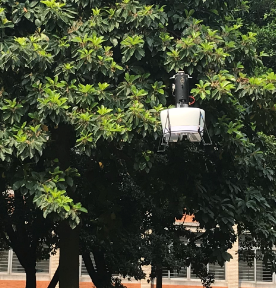
\includegraphics[scale=1]{Fig/DFUAV_f31.png} 
	% 添加标签one_DFUAV以及图标题“涵道风扇式无人机”,标题编号是自动生成的
	\caption{\label{one_DFUAV}涵道风扇式无人机} 
\end{figure}
\end{lstlisting}
其中figure为环境名,[htbp]表示将图片设置为浮动体,实际上这在.cls文件已经设置过,因而可以省略。[scale=1]表示安装1:1的比例导入图片,还可以按其他方式导入,需要时可自行百度。
\begin{figure}[htbp]
	\centering
	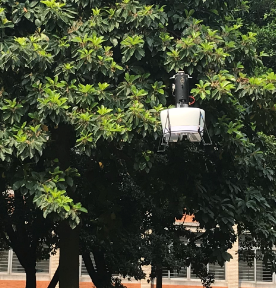
\includegraphics[scale=1]{Fig/DFUAV_f31.png}
	\caption{\label{one_DFUAV}涵道风扇式无人机}
\end{figure}

使用如下代码划分页面并排放置图\ref{Hawk}、图\ref{GTSpy}
\begin{lstlisting}
\begin{figure}[htbp]
	\centering
	\begin{minipage}[c]{0.5\textwidth} % minipage将页面划分为0.5\textwidth
		\centering
		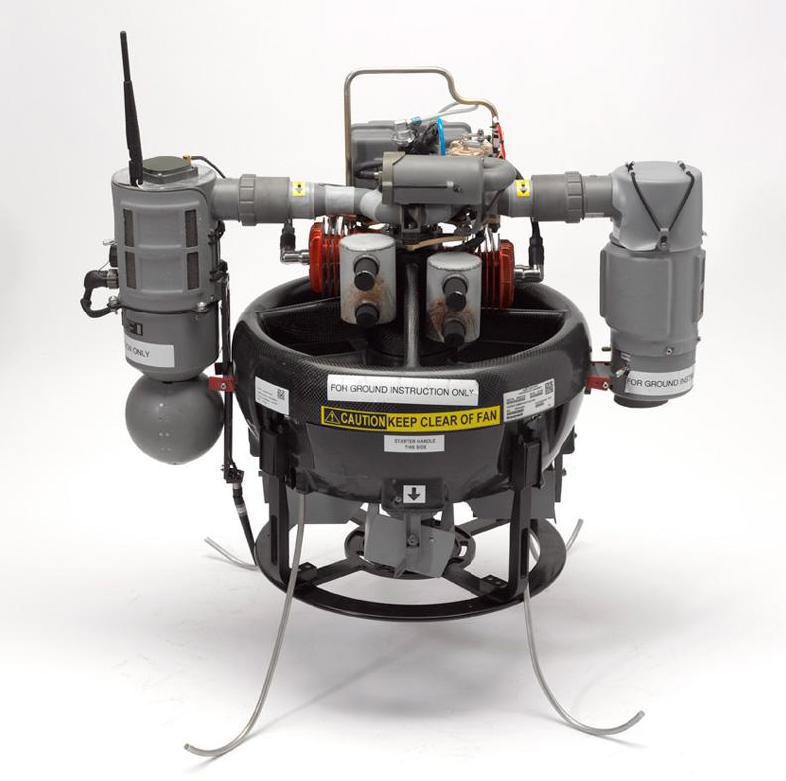
\includegraphics[width=6cm,height=6cm]{Fig/honeywell_t-hawk.jpg}
		\caption{\label{Hawk}T-Hawk}
	\end{minipage}%
	\begin{minipage}[c]{0.5\textwidth}
		\centering
		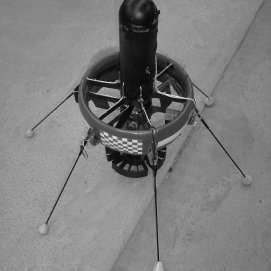
\includegraphics[width=6cm,height=6cm]{Fig/GTSpy.jpg}
		\caption{\label{GTSpy}GTSpy}
	\end{minipage}
\end{figure}
\end{lstlisting}
其中[c]表示行居中对齐。当图片大小不一但又需要1:1导入时,图标题可能行不对齐,因此可以改为如下指令:
\begin{lstlisting}
\begin{figure}[htbp]
	\centering
	\begin{minipage}[c]{0.5\textwidth}
		\centering
		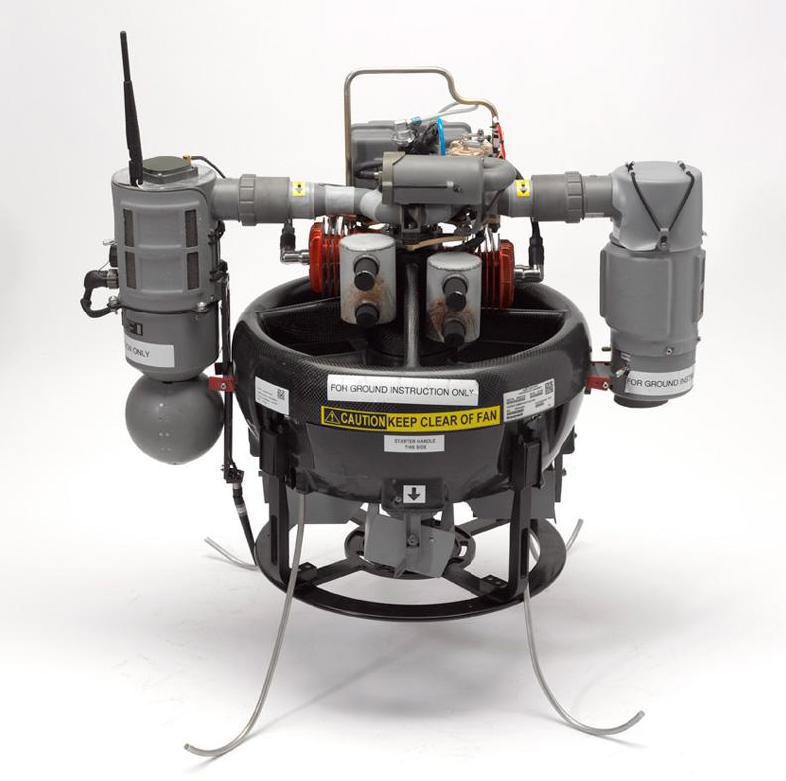
\includegraphics[scale=1]{Fig/honeywell_t-hawk.jpg} %1:1导入
	\end{minipage}%
	\begin{minipage}[c]{0.5\textwidth}
		\centering
		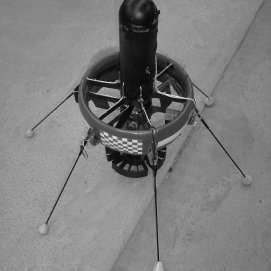
\includegraphics[scale=1]{Fig/GTSpy.jpg}
	\end{minipage}\\[1pt]
	\begin{minipage}[t]{0.5\textwidth}	% 以下为新添加页面划分,[t]表示行顶部对齐
		\caption{\label{Hawk}T-Hawk}
	\end{minipage}%
	\begin{minipage}[t]{0.5\textwidth}
		\caption{\label{GTSpy}GTSpy}
	\end{minipage}%
\end{figure}
\end{lstlisting}
\begin{figure}[htbp]
	\centering
	\begin{minipage}[c]{0.5\textwidth}
		\centering
		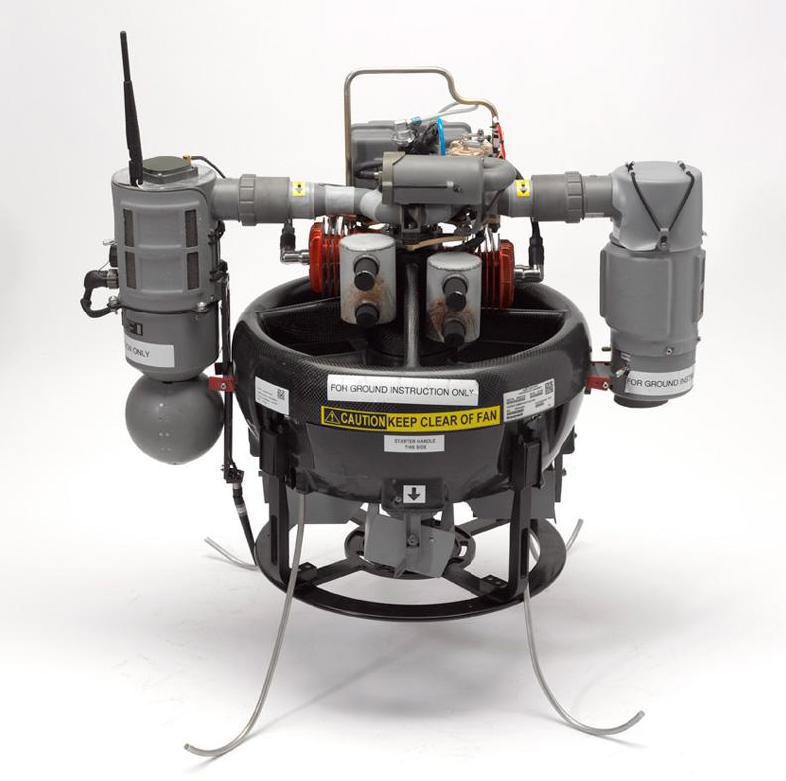
\includegraphics[width=6cm,height=6cm]{Fig/honeywell_t-hawk.jpg}
		\caption{\label{Hawk}T-Hawk}
	\end{minipage}%
	\begin{minipage}[c]{0.5\textwidth}
		\centering
		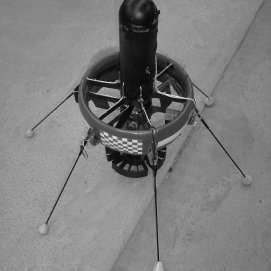
\includegraphics[width=6cm,height=6cm]{Fig/GTSpy.jpg}
		\caption{\label{GTSpy}GTSpy}
	\end{minipage}
\end{figure}
\section{表}
本节仅展示使用常见的三线表
\begin{lstlisting}
\begin{table}
	\caption{\label{TDF_para}涵道模型参数}	%表题在上
	\centering	% 表居中
	\small	% 表内字体小一号(即设置成和表题字号一致)
	\begin{tabular}{cccc}	% cccc表示4列并居中,若列之间需要分隔符则设置为|c|c|c|c|
		\hline	% \hline表示横线。列之间的元素用&分隔,\tabularnewline表示换行
		参数符号 & 数值 & 参数符号 & 数值 \tabularnewline 
		\hline 
		$I_x$ & $054593$ 		   & $I_y$ & $0.017045         $ \tabularnewline
		$l_1$ & $0.0808\,\text{m}$ & $l_2$ & $0.175\,\text{m}  $ \tabularnewline 
		$l_4$ & $0.2415\,\text{m}$ & $l_5$ & $0.1085\,\text{m} $ \tabularnewline
		\hline 
	\end{tabular}
\end{table}
\end{lstlisting}
\begin{table}
	\caption{\label{TDF_para}涵道模型参数}
	\centering
	\small 
	\begin{tabular}{cccc}
		\hline 
		参数符号 & 数值                & 参数符号 & 数值                 \tabularnewline
		\hline 
		$I_x$   & $054593$ 		     & $I_y$   & $0.017045         $ \tabularnewline
		$l_1$   & $0.0808\,\text{m}$ & $l_2$   & $0.175\,\text{m}  $ \tabularnewline 
		$l_4$   & $0.2415\,\text{m}$ & $l_5$   & $0.1085\,\text{m} $ \tabularnewline
		\hline 
	\end{tabular}
\end{table}

\section{公式}
除了前面讲行内公式,常用的还有行间公式。公式中的数学符号可自行百度,本章仅介绍常用的几种公式环境。

单独成行的行间公式在 \LaTeX{} 里由equation 环境包裹。equation 环境为公式自动生成一个编号,这个编号可以用\textbackslash{}label 和\textbackslash{}ref 生成交叉引用,amsmath 宏包的\textbackslash{}eqref 可为引用自动加上圆括号;如式\eqref{eq_1}所示。
\begin{lstlisting}
\begin{equation}
	a+b=c	\label{eq_1}
\end{equation}
\end{lstlisting}
\begin{equation}
	a+b=c	\label{eq_1}
\end{equation}
若不需要编号则加星号,改为
\begin{lstlisting}
\begin{equation*}
	a+b=c
\end{equation*}
\end{lstlisting}
其他环境类似。当使用 \texttt\$ 开启行内公式输入,或是使用{equation} 环境时,\LaTeX\ 就进入了数学模式。
数学模式相比于文本模式有以下特点:
\begin{enumerate}
	\item 数学模式中输入的空格被忽略。数学符号的间距默认由符号的性质(关系符号、运算符等)决定。
	需要人为引入间距时,使用 \textbackslash{}{quad} 和 \textbackslash{}{qquad} 等命令。
	\item {不允许有空行(分段)}。行间公式中也无法用 $ \verb|\\|$命令手动换行。排版多行公式需要用到 其他各种环境。
	\item 所有的字母被当作数学公式中的变量处理,字母间距与文本模式不一致,也无法生成单词之间的空格。
	如果想在数学公式中输入正体的文本,简单情况下可用 \textbackslash{}{mathrm} 命令。
	或者用 {amsmath} 提供的 \textbackslash{}{text} 命令(仅适合在公式中穿插少量文字。如果你的情况正好相反,需要在许多文字中穿插使用公式,则应该像正常的行内公式那样用,而不是滥用 \textbackslash{}{text} 命令)。
\end{enumerate}	

实际上更常用的的是多行公式,不需要对齐的公式组可以使用gather环境,需要对齐的公式组用align 环境。
长公式内可用$ \verb|\\|$ 换行。

如果需要罗列一系列公式,并令其按照等号对齐,可用align 环境,它将公式用\& 隔为两部分并对齐。分隔符通常放在等号左边:
\begin{lstlisting}
\begin{align}
	a & = b + c \\
	& = d + e
\end{align}
\end{lstlisting}
\begin{align}
a & = b + c \\
& = d + e
\end{align}
align 环境会给每行公式都编号。

如果不需要按等号对齐,只需罗列数个公式,可用gather环境:
\begin{lstlisting}
\begin{gather}
	a  = b + c \notag \\
	f = d + e 
\end{gather}
\end{lstlisting}
\begin{gather}
	a  = b + c \notag  \\
	f = d + e 
\end{gather}
gather 环境同样会给每行公式都编号,如果某行不需要编号可在行末用\textbackslash{}notag 仅去掉某行的编号。

align 和gather 有对应的不带编号的版本align* 和gather*。

另一个常见的需求是将多个公式组在一起公用一个编号,编号位于公式的居中位置。为此,
amsmath 宏包提供了诸如aligned、gathered 等环境,与equation 环境套用。以-ed 结尾的
环境用法与前一节不以-ed 结尾的环境用法一一对应。我们仅以aligned 举例:
\begin{lstlisting}
\begin{equation}
	\begin{aligned}
		a &= b + c \\
		d &= e + f + g \\
		h + i &= j + k \\
		l + m &= n
	\end{aligned}
\end{equation}
\end{lstlisting}
\begin{equation}
	\begin{aligned}
		a &= b + c \\
		d &= e + f + g \\
		h + i &= j + k \\
		l + m &= n
	\end{aligned}
\end{equation}
split 环境和aligned 环境用法类似,也用于和equation 环境套用,区别是split 只能
将每行的一个公式分两栏,aligned 允许每行多个公式多栏。

分段函数通常用amsmath 宏包提供的cases 环境,可参考文献\parencite{_c}

amsmath 宏包还直接提供了多种排版矩阵的环境,包括不带定界符的matrix,以及带各种定界符的矩阵pmatrix、bmatrix、Bmatrix、vmatrix、Vmatrix。
其中中括号版的bmatrix最常用。这些矩阵环境需要在公式中使用,比如 align 环境。
\begin{lstlisting}
A= \begin{bmatrix}
		x_{11} & x_{12} & \ldots & x_{1n} \\
		x_{21} & x_{22} & \ldots & x_{2n} \\
		\vdots & \vdots & \ddots & \vdots \\
		x_{n1} & x_{n2} & \ldots & x_{nn}
	\end{bmatrix}
\end{gather}
\end{lstlisting}
\begin{gather}
\bm{A}= \begin{bmatrix}
	x_{11} & x_{12} & \ldots & x_{1n} \\
	x_{21} & x_{22} & \ldots & x_{2n} \\
	\vdots & \vdots & \ddots & \vdots \\
	x_{n1} & x_{n2} & \ldots & x_{nn}
   \end{bmatrix}
\end{gather}	
其中矩阵/向量加粗使用\textbackslash{}bm\{\}命令。另外还可以使用array环境排版矩阵,类似tabular环境,用$ \verb|\\|$ 和\& 用来分隔行和列,这里不再赘述。	
\begin{lstlisting}
\begin{array }[外部对齐tcb]{列对齐lcr}
	行列内容
\end{array}
\end{lstlisting}

另外注意排版分式时,有两种方法:\textbackslash{}frac或者\textbackslash{}dfrac,效果分别为$ \frac{1}{2} $和$ \dfrac{1}{2} $。以上介绍的数学环境中,空格可参考文献\parencite{_c},例如常用\textbackslash{}quad。
\section{定理}
在scutthesis.cls文件536行开始,已经用\textbackslash{}newtheorem命令定义了几种定理环境,包括:定义、假设、定理、结论、引理、公理、推论、性质等等,统称定理环境,关于\textbackslash{}newtheorem的用法,可参考\cite{_c}或自行百度。要下面提供几个例子,在横线之间的深色区域是代码,效果在相应下方表示:
\begin{lstlisting}
\begin{assumption}
	加权矩阵${{\bm{W}}_{1}}$和 ${{\bm{W}}_{2}}$ 是对称矩阵,且$ {{\bm{W}}_{2}}$非奇异。	\label{assum_dca1}
\end{assumption}
\end{lstlisting}
\begin{assumption}
	加权矩阵${{\bm{W}}_{1}}$和 ${{\bm{W}}_{2}}$ 是对称矩阵,且$ {{\bm{W}}_{2}}$非奇异。	\label{assum_dca1}
\end{assumption}

定理用法和假设类似:
\begin{lstlisting}
\begin{theorem}
	如果假设\ref{assum_dca1}成立,$\bm{F}$满足式\eqref{eq_F}的定义,且${{\bm{W}}_{1}}$非奇异,则有$0\le e \left( \bm{F} \right) < 1$,其中$e \left( \bm{F} \right)$是 $\bm{F}$的特征值。	\label{the_dca2}
\end{theorem}
\end{lstlisting}
\begin{theorem}
	如果假设\ref{assum_dca1}成立,$\bm{F}$满足上式的定义,且${{\bm{W}}_{1}}$非奇异,则有$0\le e \left( \bm{F} \right) < 1$,其中$e \left( \bm{F} \right)$是 $\bm{F}$的特征值。	\label{the_dca2}
\end{theorem}

定理环境的编号可自定义,但通常不需要再进行设置,因为模板文件scutthesis.cls文件已经定义好。
\section{参考文献}

\begin{lstlisting}
关于参考文献这块,很多同学有疑问。只有记住一点:不管用什么参考文献管理工具,最终目的是生成一个bib文件给TeXstudio使用,bib文件里是特定格式的文献信息。bib文件可以使用一个叫notepad++的软件打开。
\end{lstlisting}

通常学位论文参考文献是基于BibTeX进行的,本模板最大的改进就是引入BibLaTeX。关于这部分知识可参考文献\parencite{_c,_g}的第六章,6.1节参考文献和BIBTEX工具。

参考文献引用和著录是基于ZOTERO这个软件进行的。视频教程见\parencite{_k}。此外,为了符合毕业论文撰写规范,需设置参数。按照视频教程安装完必要的插件(如Better BibTeX)后,在编辑->首选项进行设置。附录图\ref{op1}到图\ref{op11}所示的是我的zotero软件设置。其中最重要的是\ref{op10}的设置要排除的选项,多余的显示会让审稿人反感,按照论文撰写规范进行即可。在毕业论文撰写时,在编辑->首选项->Better BibLTeX->Fields中,Fields to omit from export填month,abstract,note,extra,file,keywords,type,url,doi,就是在参考文献著录中排除这些多余的项,避免过于复杂。而在写本模板使用说明时,没有排除url,因为很多参考资料是网页。

\begin{lstlisting}
使用zotero,科学上网很重要,通常我们使用谷歌学术搜索文献并利用chrome的zotero插件直接捕获文献著录信息。但我使用蓝灯,代理服务器均遇到过被谷歌学术封锁的情况。只能不断换科学上网方法。这里我现在用的chrome插件:谷歌上网助手,它可以轻松捕获谷歌学术的著录信息,注册一个账号即可使用。谷歌上网助手有可能和某些代理冲突。这些都是科学上网的问题,已经超出了本项目的范围,听说百度一下 v2ray 可发现新大陆,可惜我试了Vultr的服务器依然被谷歌封。知网捕获中文参考文献著录信息的话不需要考虑这个问题,直接在知网首页搜索文献然后点击插件既可以选想捕获的著录了。
\end{lstlisting}

在zotero软件点击文件->导出文献库,如图\ref{output}所示,再在导出对话框图\ref{output_format}选择导出格式为Better BibLaTeX,同时勾选Keep updated选项保持自动更新,再点击ok,在弹出的对话框图\ref{output_name}确定保存路径和文件名,例如我的是MyLibrary.bib,这也是我整个读书生涯的文献库bib文件。如果写小论文的话通常导出格式是BibTeX或者Better BibTeX(这里按照期刊的要求来即可,文献管理软件的好处就是快速自动生成一个文件库)。关于BibTeX和BibLaTeX的区别这里不做展开。

得到文献库后,在scutthesis.tex文件第九行使用\textbackslash{}addbibresource命令,添加文献库。引用某文献时秩序在zotero选中某文献条目,然后按Ctrl+Shift+C,复制引用关键字(Citation Key)到剪切板(快捷键可自定义)。然后在tex文件编辑界面直接粘贴,默认的时上标形式,若需要非上标形式,可以改为\textbackslash{}parencite{XXXX},其中XXXX是Citation Key。这里的操作和认为设置的首选项参数有关,需要在编辑->首选项->导出界面的默认格式一栏选中相应的项,同时在编辑->首选项->高级->快捷键设置为默认值。

---------------------------------------------------------------------------------

2020年12月2日测试:
下载最新zotero,从知网和谷歌捕获文献(刚打开网页最好稍等一会再点击插件,谷歌可能需要现人机验证),对文献\parencite{Renduchintala_2019}、\parencite{Meng_2020}进行引用。

---------------------------------------------------------------------------------
\begin{lstlisting}
另外有同学反映,换了电脑后重新导出的bib文件Citation Key值不同,记得设置好Better BibTeX之后,在著录条目界面全选著录(或仅选想更新的著录)然后右键选Better BibTeX更新refresh一下。然后在Automatic export选项点击Export now立即更新bib文件(按理说勾选了自动更新选项他会自动更新,但为了确保万无一失还是点一下)。
\end{lstlisting}










 % 第三章
% 自行根据需要添加章节。
...
\chapter{结\texorpdfstring{\quad}{}论}
本文主要是展示如何使用修改“祖传模板”得到的新模板,在使用时直接替换成自己的论文内容即可。总结下来最最最麻烦的是科学上网,只有科学上网才能获取文献信息生成bib文件,后面就好办了。

本模板难免有不足之处,主要是我本人的论文涉及的格式有限,有些地方没探索到自然就没去设置。比如附录,附录的图文并茂等等,我本人是没有研究的,这里仅仅做了一些初步的工作,不过对很多同学来说本模板是够用的。希望有能帮助到华工的同学们,有不足之处请多多理解,可以通过邮件联系我,上班之余我会尽量回复。 % 结论
...
\printbibliography	% 参考文献著录
\chapter{附\texorpdfstring{\quad}{}录}
\renewcommand{\thesection}{{附录}\arabic{section}}
\setcounter{section}{0}
\section{zotero的设置}
\begin{figure}
	\centering
	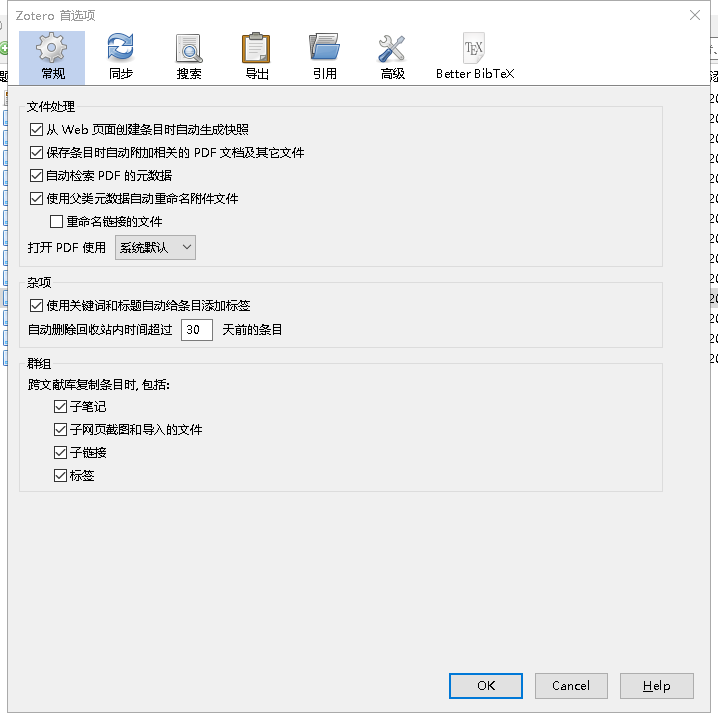
\includegraphics[scale=0.8]{Fig/zotero1.png}
	\caption{\label{op1}常规}
\end{figure}
\begin{figure}
	\centering
	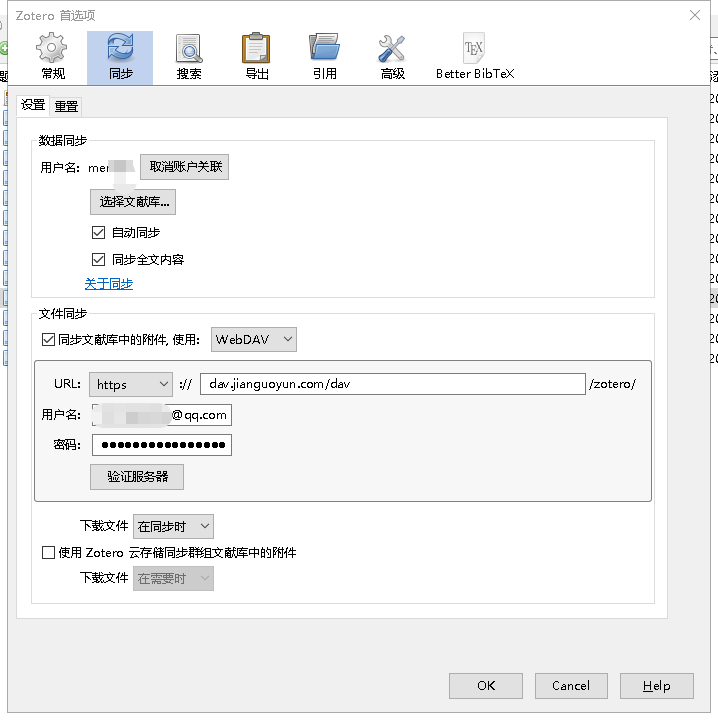
\includegraphics[scale=0.8]{Fig/zotero2.png}
	\caption{\label{op2}同步1}
\end{figure}
\begin{figure}
	\centering
	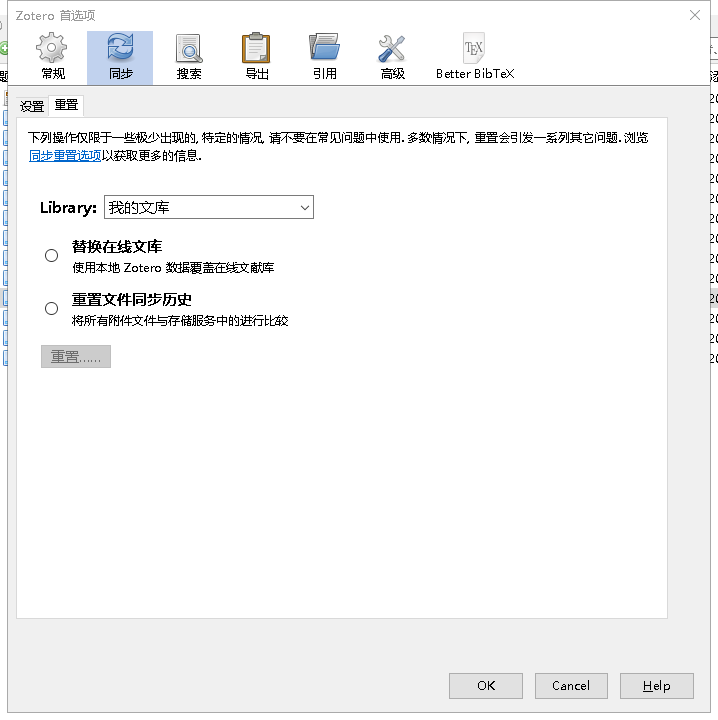
\includegraphics[scale=0.8]{Fig/zotero3.png}
	\caption{\label{op3}同步2}
\end{figure}
\begin{figure}
	\centering
	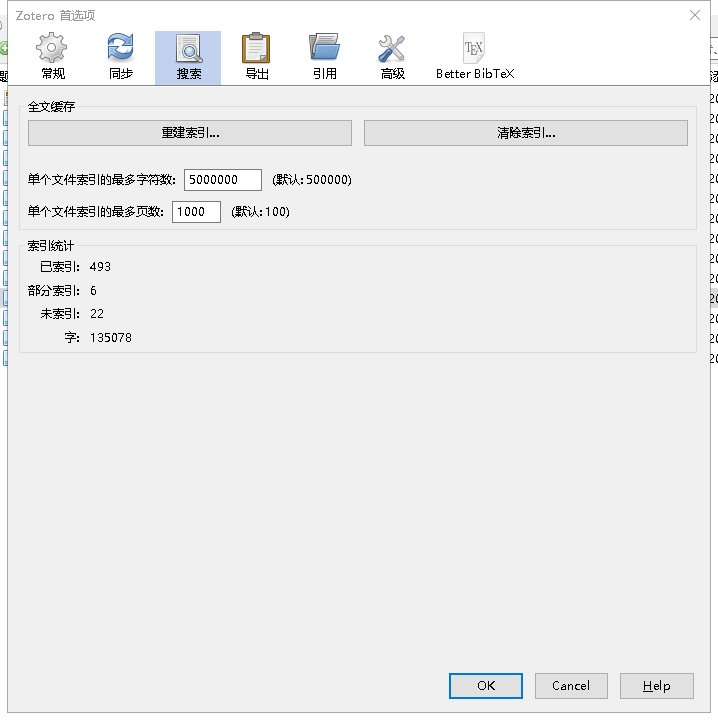
\includegraphics[scale=0.8]{Fig/zotero4.png}
	\caption{\label{op4}搜索}
\end{figure}
\begin{figure}
	\centering
	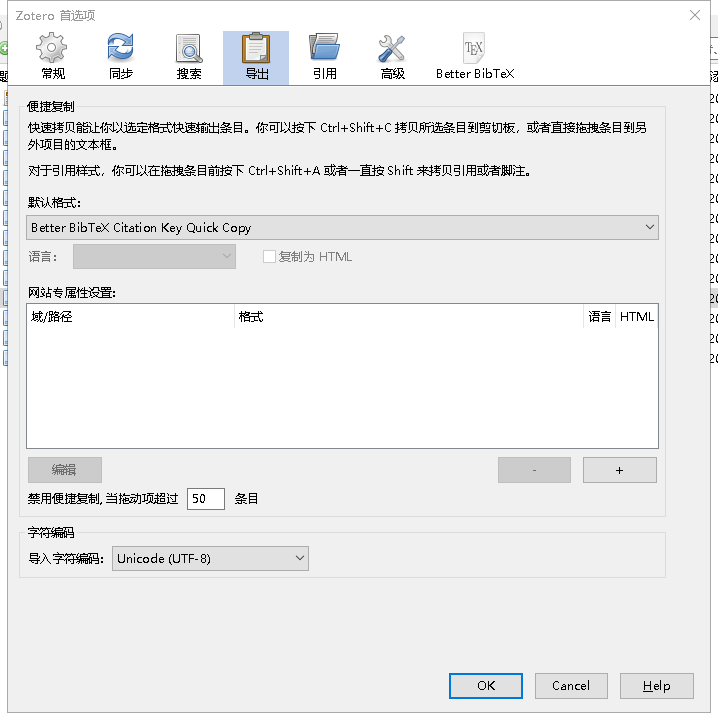
\includegraphics[scale=0.8]{Fig/zotero5.png}
	\caption{\label{op5}导出}
\end{figure}
\begin{figure}
	\centering
	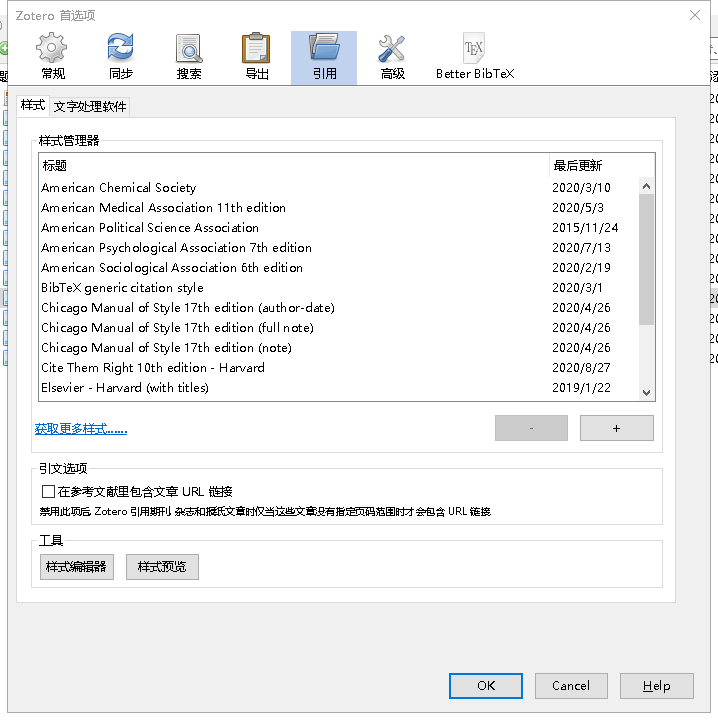
\includegraphics[scale=0.8]{Fig/zotero6.png}
	\caption{\label{op6}引用}
\end{figure}
\begin{figure}
	\centering
	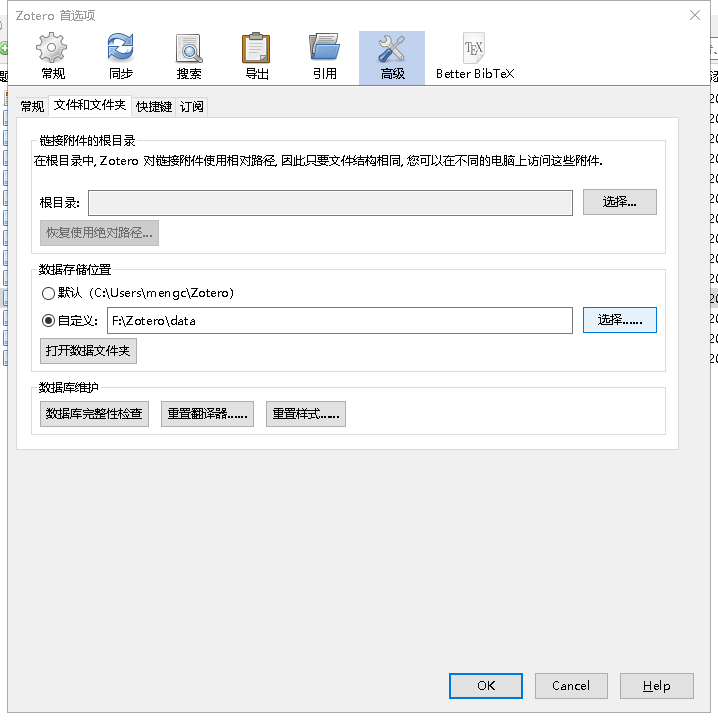
\includegraphics[scale=0.8]{Fig/zotero7.png}
	\caption{\label{op7}高级1}
\end{figure}
\begin{figure}
	\centering
	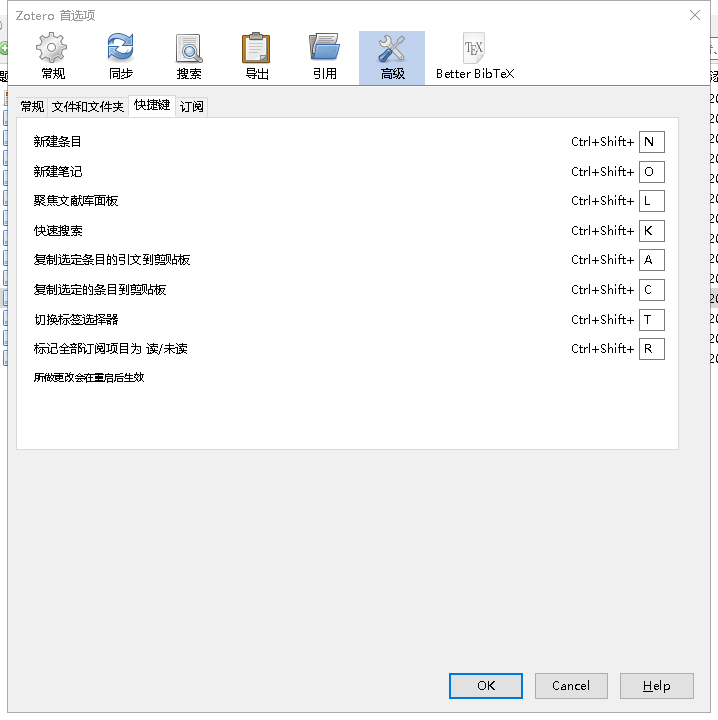
\includegraphics[scale=0.8]{Fig/zotero8.png}
	\caption{\label{op8}高级2}
\end{figure}
\begin{figure}
	\centering
	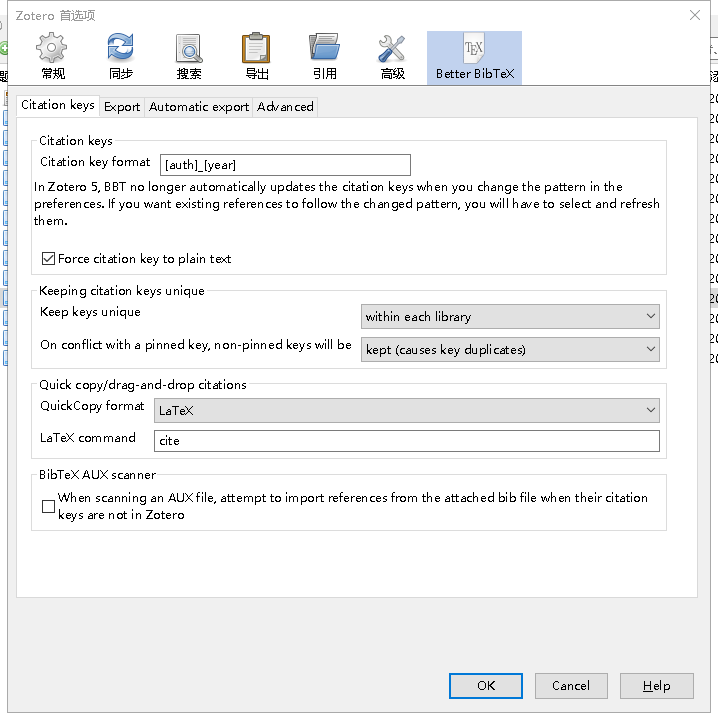
\includegraphics[scale=0.8]{Fig/zotero9.png}
	\caption{\label{op9}Better BibTeX1}
\end{figure}
\begin{figure}
	\centering
	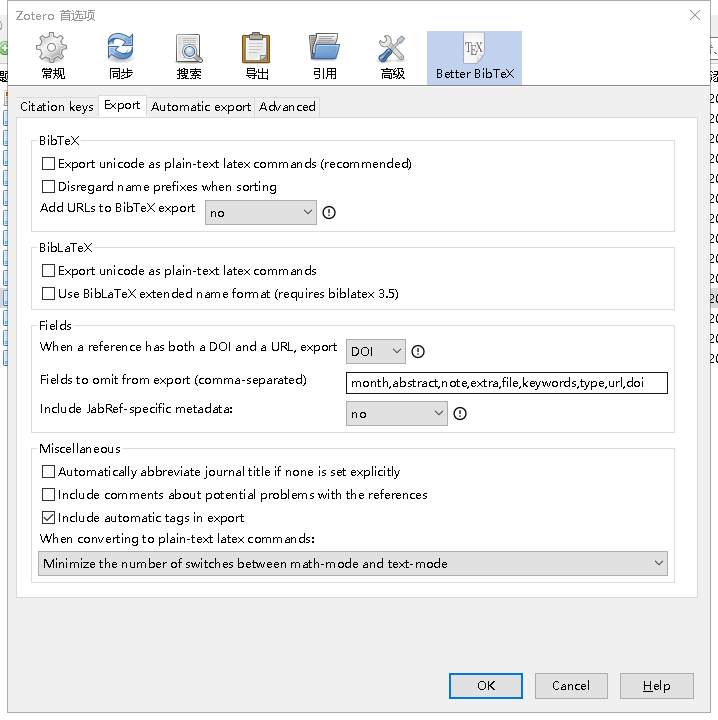
\includegraphics[scale=0.8]{Fig/zotero10.png}
	\caption{\label{op10}Better BibTeX2}
\end{figure}
\begin{figure}
	\centering
	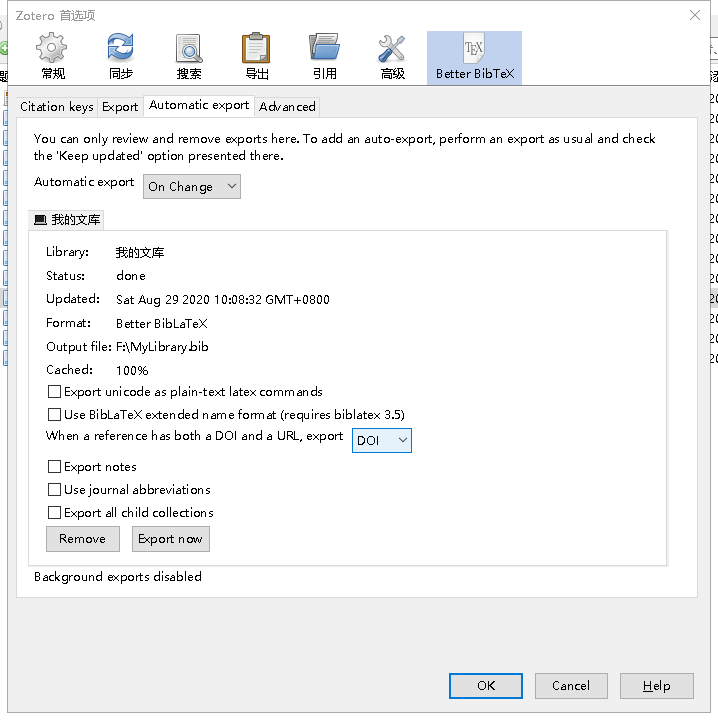
\includegraphics[scale=0.8]{Fig/zotero11.png}
	\caption{\label{op11}Better BibTeX3}
\end{figure}

\begin{figure}[htbp]
	\centering
	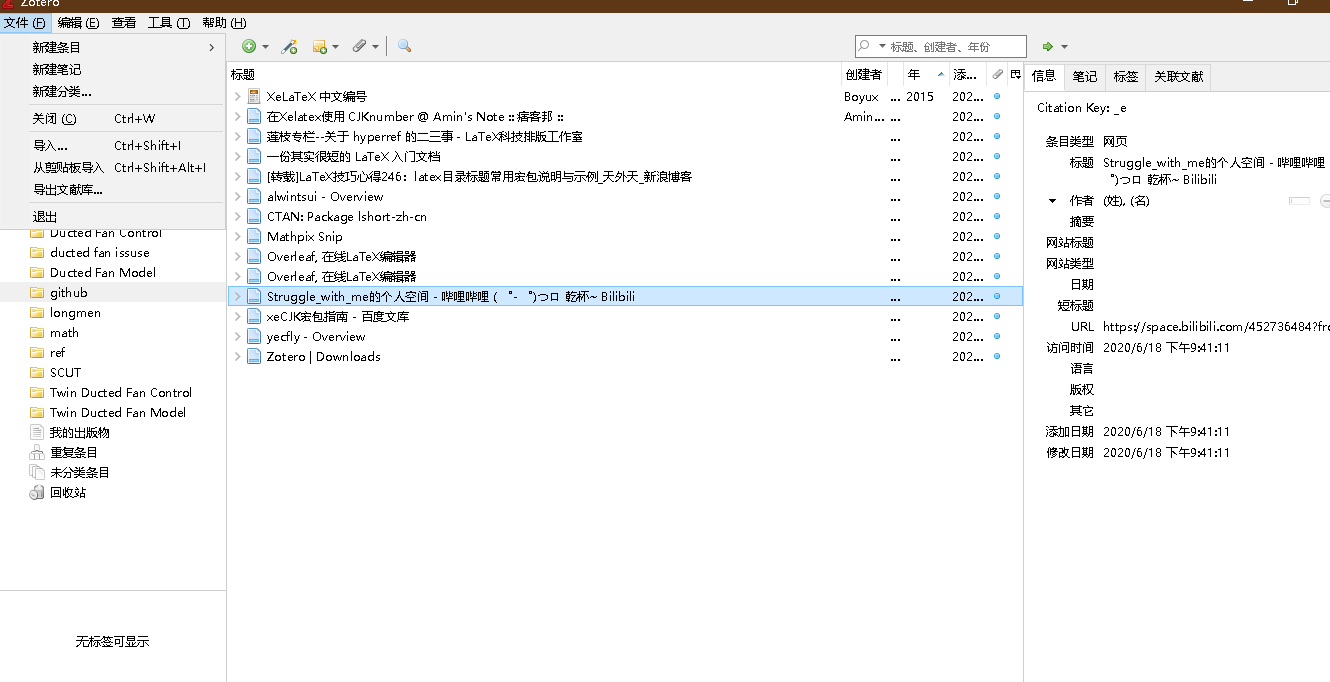
\includegraphics[scale=0.42]{Fig/zotero12.png}
	\caption{\label{output}导出文献库}
\end{figure}

\begin{figure}[htbp]
	\centering
	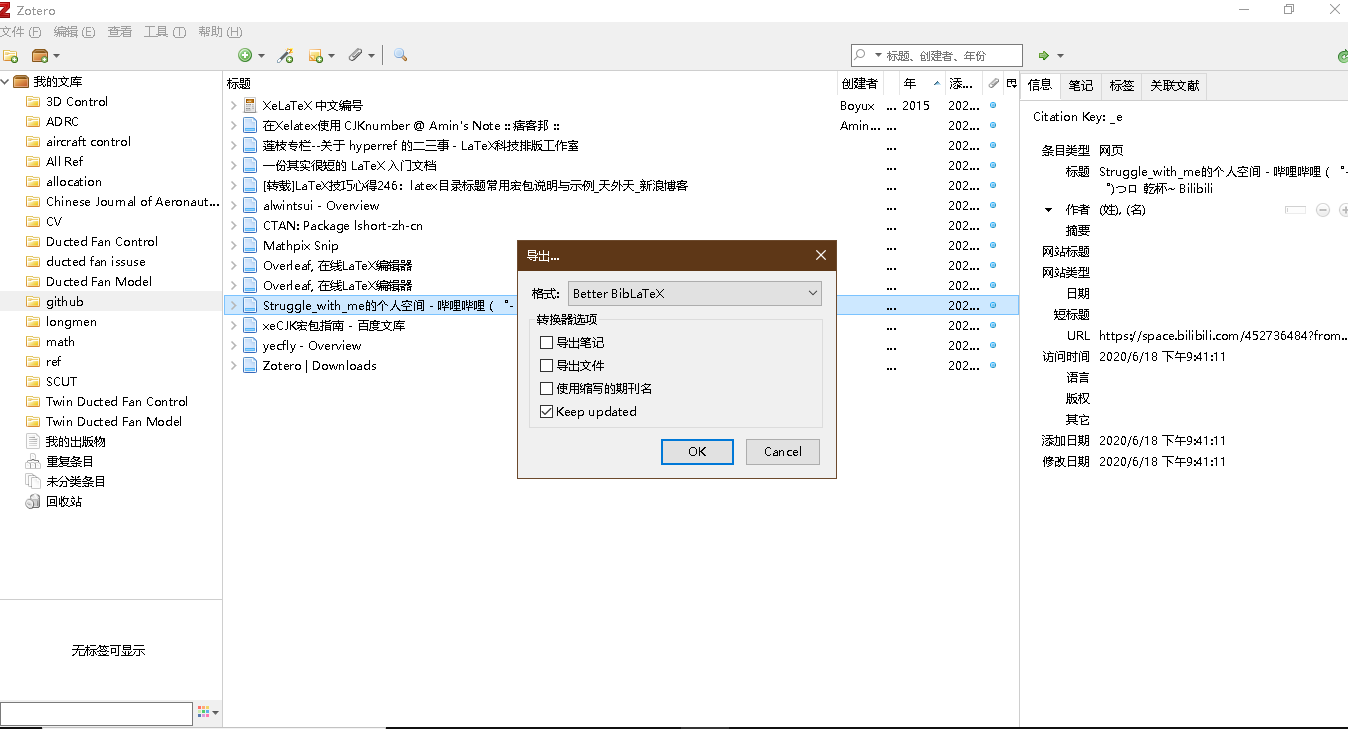
\includegraphics[scale=0.42]{Fig/zotero13.png}
	\caption{\label{output_format}导出格式}
\end{figure}

\begin{figure}[htbp]
	\centering
	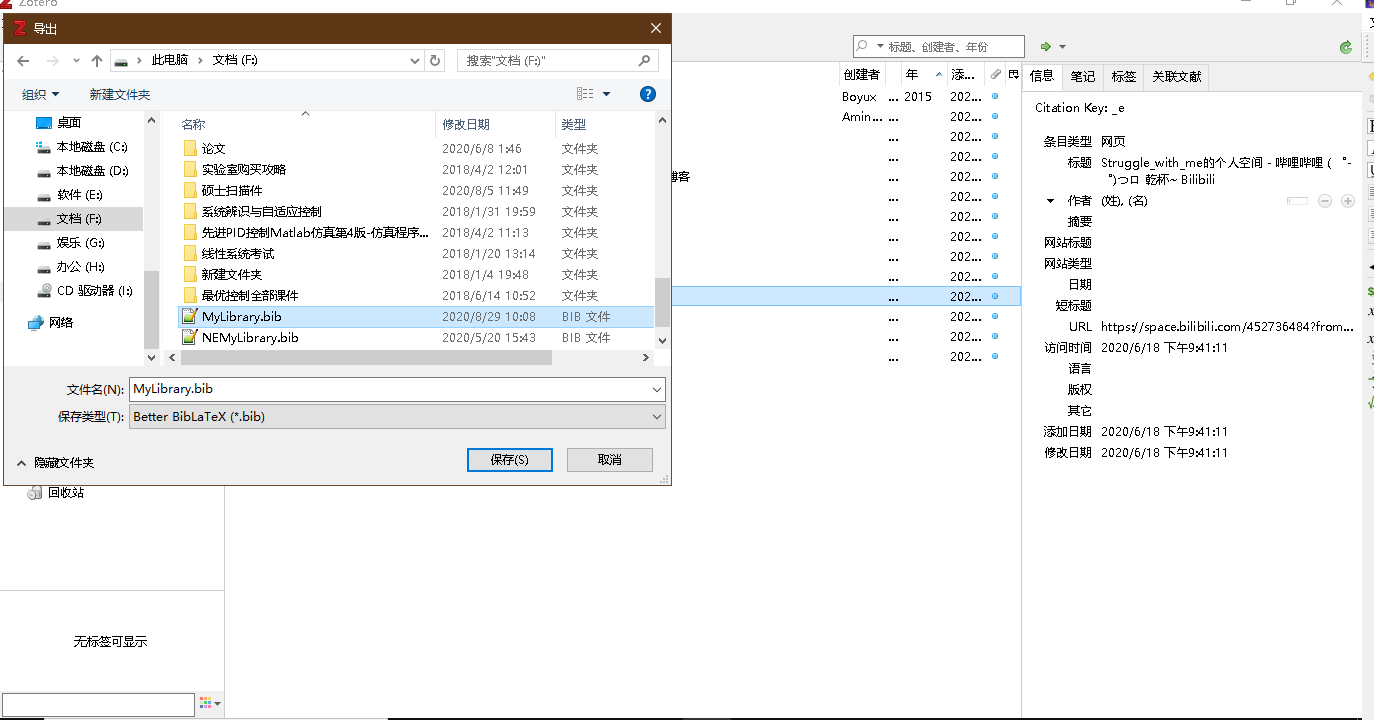
\includegraphics[scale=0.42]{Fig/zotero14.png}
	\caption{\label{output_name}导出文件名}
\end{figure}
\section{BibLatex}

 % 附录
\chapter{攻读硕士学位期间取得的研究成果}
已发表(包括已接受待发表)的论文,以及已投稿、或已成文打算投稿、或拟成文投稿的论文情况(只填写与学位论文内容相关的部分):
\begin{table}
	\centering{}%
	\small 
	\begin{longtable}{|>{\centering}m{0.5cm}|m{1.8cm}|>{\centering}m{2.8cm}|>{\centering}m{2.5cm}|>{\centering}m{2.2cm}|>{\centering}m{2.cm}|>{\centering}m{1cm}|}
		\hline 
		序号 & 作者(全体作者,按顺序排列) & 题 目 						   & 发表或投稿刊物名称、级别 & 发表的卷期、年月、页码 & 相当于学位论文的哪一部分(章、节) & 被索引收录情况\tabularnewline
		\hline 
		1    & 蒙超恒、裴海龙、程子欢					  & 涵道风扇式无人机的优先级控制分配 & 航空学报 & 已录用,2020年5月 & 2.1、2.2、3.4、4.1、4.2、5.1和5.3节 & EI\tabularnewline
		\hline 
		2	 & 	蒙超恒、裴海龙、程子欢						&  	Dynamic Control Allocation for A Twin Ducted Fan UAV							 & 2020 International Conference on Guidance, Navigation and Control  & 已录用,2020年8月 & 2.3、4.3和5.2节 &EI \tabularnewline
		\hline 
	\end{longtable}
\end{table}

注:在“发表的卷期、年月、页码”栏:

1.如果论文已发表,请填写发表的卷期、年月、页码;

2.如果论文已被接受,填写将要发表的卷期、年月;

3.以上都不是,请据实填写“已投稿”,“拟投稿”。

不够请另加页。

二、与学位内容相关的其它成果(包括专利、著作、获奖项目等)



%注:这部分一言难尽,我努力了很久都没有把这个表做好。感觉学校给的这个表的模板非常反人类。看国外大学的博士论文,那种像参考文献著录信息那样一行一行的,比较美观。而这个框框很难放文字进去。 % 成果
\chapter{致\texorpdfstring{\quad}{}谢}
%把下面文字替换
\begin{center}
这次你离开了没有像以前那样说再见,再见也他妈的只是再见 
~\\
我们之间从来没有想象的那么接近,只是两棵树的距离 
~\\
你是否还记得山阴路我八楼的房间,房间里唱歌的日日夜夜 
~\\
那么热的夏天你看着外面,看着你在消逝的容颜 
~\\
我多么想念你走在我身边的样子,想起来我的爱就不能停止 
~\\
南京的雨不停地下不停地下,就像你沉默的委屈 
~\\
一转眼,我们的城市又到了夏天,对面走来的人都眯着眼 
~\\
人们不敢说话不敢停下脚步,因为心动常常带来危险 
~\\
我多么想念你走在我身边的样子,想起来我的爱就不能停止 
~\\
南京的雨不停地下不停地下,有些人却注定要相遇 
~\\
你是一片光荣的叶子,落在我卑贱的心 
~\\
像往常一样我为自己生气并且歌唱 
~\\
那么乏力,爱也吹不动的叶子 
\end{center}
%把上面文字替换

~\\

\begin{minipage}[t]{0.945\textwidth}%
	\begin{flushright}
		蒙超恒\\
		\today\\	% 时间
		于华南理工大学
		\par\end{flushright}
\end{minipage}

 % 致谢
\end{lstlisting}
其中$\%$之后的内容为注释,...表示省略其他代码,仅保留论文内容主体部分。\textbackslash{}include\{xxx\}指令用于包含xxx.tex文件的内容,各章节的内容主要在xxx.tex中保存。在\textbackslash{}documentclass 和\textbackslash{}begin\{document\} 之间的位置称为导言区。在导言区中一般会使用\textbackslash{}usepackage 调用宏包,以及会进行对文档的全局设置。本模板的导言区除调用所需的宏包外,还进行了页眉页脚的设置。有的模板会把所有调用宏包的指令放到一个.sty宏包文件中,页面的设置放在文档类文件.cls文件中。因本人时间有限,就不做整理,欢迎有志之士加入完善。使用本模板并不需要了解导言区的指令,在需要时额外添加即可(要注意宏包冲突)。特别地,\textbackslash{}includeonly\{xxx\}指令用于使文档仅编译xxx.tex文件的内容,这就是分章节包含(include)的好处,可大大减少编译时间。

将封面打印保存为 thesis\_cover.pdf 文件,硕士使用master\_cover.docx ,博士使用 doctor\_cover.doc 。如果有更新版本的封面,可自行替换。文档类默认是博士论文,下面指令将控制添加封面与否:
\begin{lstlisting}
\documentclass[unicode,master,pdfcover]{scutthesis}	% 使用pdf文件封面的 硕士模板
\documentclass[unicode,master]{scutthesis}	% 不使用pdf文件封面的 硕士模板
\documentclass[unicode,pdfcover]{scutthesis}	% 使用pdf文件封面的博士模板
\documentclass[unicode]{scutthesis}	% 不使用pdf文件封面的博士模板
\end{lstlisting}
不使用thesis\_cover.pdf 文件指定的封面时,将使用草稿封面。草稿封面也可以减少编译时间,因此可以在最终提交论文时再使用论文封面。草稿封面用以下指令设置:
\begin{lstlisting}
%%%%%%%%%%%%%草稿封面设置%%%%%%%%%%%%%	
\title{LaTeX模板}	
\author{蒙超恒}	
\supervisor{指导教师:裴海龙\ 教授}	
\institute{华南理工大学}	
\date{2020年5月20日}
%%%%%%%%%%%%%%%%%%%%%%%%%%%%%%%%%%%%%
\end{lstlisting}
\section{章节文件}
章节文件如chapter0x.tex等,其内容由\textbackslash{}chapter\{章名\}开头。新建一章可新建一个文件并由\textbackslash{}chapter\{新建章名\}开头填写内容即可。节及小节分别用\textbackslash{}section\{新建节名\}、\textbackslash{}subsection\{新建小节名\}命令。

正文的的书写和txt文本文件的书写类似。\LaTeX{} 源代码中,空格键和Tab键输入的空白字符视为“空格”。连续的若干个空白字符视为一个空格。一行开头的空格忽略不计。行末的回车视为一个空格;但连续两个回车,也就是空行,会将文字分段。多个空行被视为一个空行。也可以在行末使用\textbackslash{}par 命令分段。在本模板中,英文之间的空格被保留,中文之间的空格被忽略。特别地,摘要,附录,结论等两个字的大纲级别为章的章名,中间使用空格隔开。对此论文撰写规范并没有明文要求,只是为了美观。也可以全部不加空格。一般情况下,在文本文字中添加空格使用\textbackslash{}quad命令,但由于文献\parencite{_d}所述原因,直接使用\textbackslash{}quad命令会报警,因而使用\textbackslash{}texorpdfstring\{\textbackslash{}quad\}\{\},其中最后一个\{\}里面可以加一个空格,不影响使用。目录二字之间添加空格在scutthesis.cls文件317行设置。

正文本环境中使用公式,即行内公式,需要用两个\$包围,如源码:\$a+b=c\$ 显示为$a+b=c$。使用其他字符可自行百度或阅读参考文献。再次提醒,使用\LaTeX{}撰写论文不需要研究其原理,在达到某种效果(图文显示、公式显示效果)时百度或查书寻找其代码即可。

综上,论文撰写只需要将自己的文本(包含行内公式)放到相应的章节处,并添加行间公式、图表环境并填写图表即可。行间公式、图表将在下一章介绍。

 % 第二章

\chapter{常用环境及参考文献设置}
强烈建议在使用公式、表格、定理环境时进行百度,没必要研究各种用法,只需要知道自己需要什么。因本人的论文所用表格较少,因而对表格不是很熟悉,本章对表格的介绍相应的较少。本章仅介绍本人在论文撰写过程中常用的环境以及参考文献设置。

\section{图}
图的导入需要提前准备好图片文件,最好是.png、.eps、.pdf或.jpg文件。另外,如果是从matlab导出图片文件,可使用print函数或手动导出,print函数的使用可参考ICGNC2020plot.m以及PlotToFileColorPDF.m文件等。手动导出(matlab的figure界面的“文件”->“导出设置”设置好大小分辨率和线宽等然后点击“应用于图窗”)主要用于观察效果,可设置某种导出样式后导出该样式,下次使用时加载,具体可百度“matlab导出高清图片”。需要特别注意的是一定要1:1导入matlab生成的图片,并且图中文字设置好字体字号。

使用如下代码放置独立成行的图片,效果如图\ref{one_DFUAV}所示
\begin{lstlisting}
\begin{figure}[htbp]
	% 图片居中(列居中对齐)
	\centering	
	% 包含当前路径下的Fig文件夹的图片文件DFUAV_f31.png
	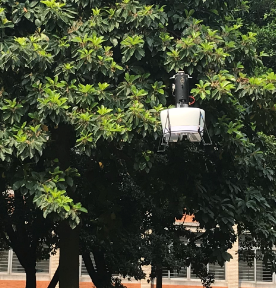
\includegraphics[scale=1]{Fig/DFUAV_f31.png} 
	% 添加标签one_DFUAV以及图标题“涵道风扇式无人机”,标题编号是自动生成的
	\caption{\label{one_DFUAV}涵道风扇式无人机} 
\end{figure}
\end{lstlisting}
其中figure为环境名,[htbp]表示将图片设置为浮动体,实际上这在.cls文件已经设置过,因而可以省略。[scale=1]表示安装1:1的比例导入图片,还可以按其他方式导入,需要时可自行百度。
\begin{figure}[htbp]
	\centering
	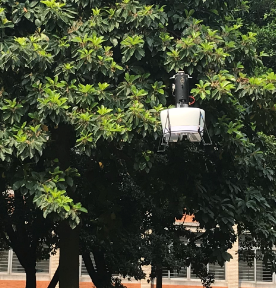
\includegraphics[scale=1]{Fig/DFUAV_f31.png}
	\caption{\label{one_DFUAV}涵道风扇式无人机}
\end{figure}

使用如下代码划分页面并排放置图\ref{Hawk}、图\ref{GTSpy}
\begin{lstlisting}
\begin{figure}[htbp]
	\centering
	\begin{minipage}[c]{0.5\textwidth} % minipage将页面划分为0.5\textwidth
		\centering
		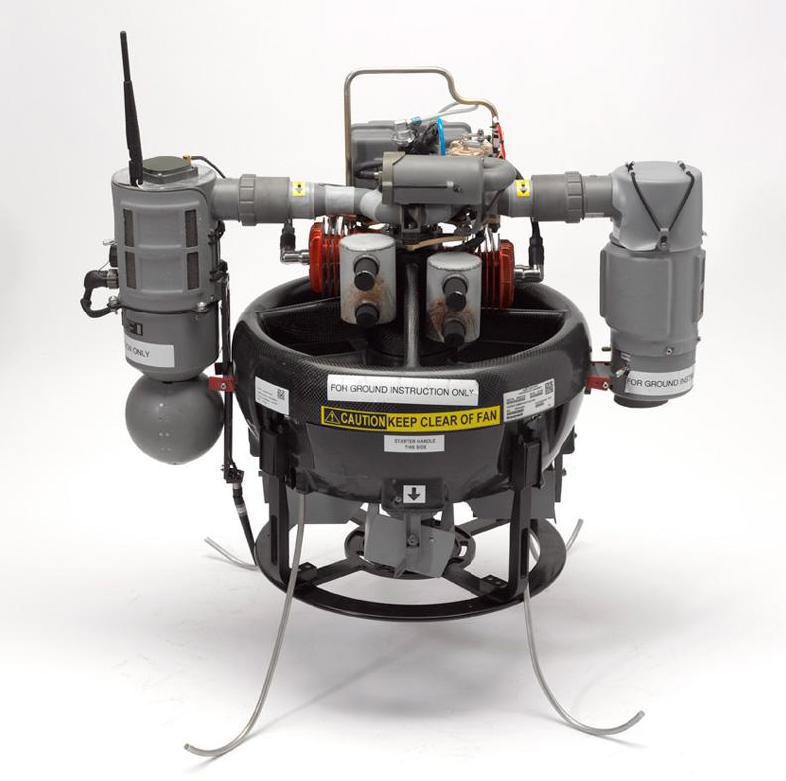
\includegraphics[width=6cm,height=6cm]{Fig/honeywell_t-hawk.jpg}
		\caption{\label{Hawk}T-Hawk}
	\end{minipage}%
	\begin{minipage}[c]{0.5\textwidth}
		\centering
		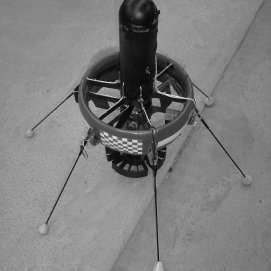
\includegraphics[width=6cm,height=6cm]{Fig/GTSpy.jpg}
		\caption{\label{GTSpy}GTSpy}
	\end{minipage}
\end{figure}
\end{lstlisting}
其中[c]表示行居中对齐。当图片大小不一但又需要1:1导入时,图标题可能行不对齐,因此可以改为如下指令:
\begin{lstlisting}
\begin{figure}[htbp]
	\centering
	\begin{minipage}[c]{0.5\textwidth}
		\centering
		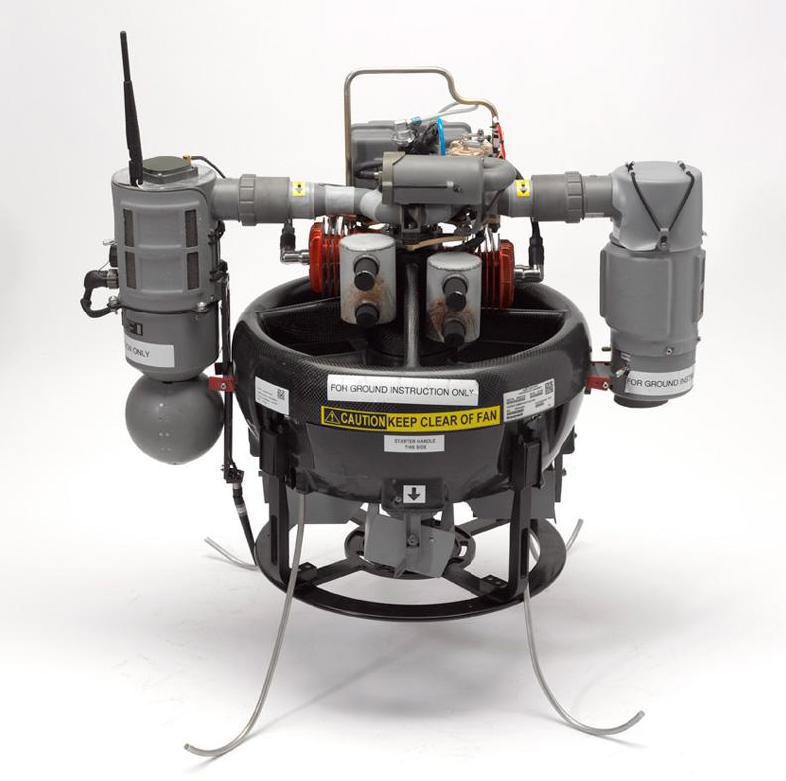
\includegraphics[scale=1]{Fig/honeywell_t-hawk.jpg} %1:1导入
	\end{minipage}%
	\begin{minipage}[c]{0.5\textwidth}
		\centering
		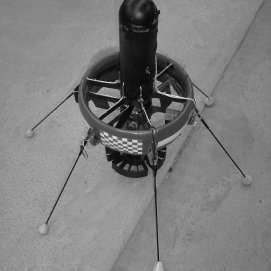
\includegraphics[scale=1]{Fig/GTSpy.jpg}
	\end{minipage}\\[1pt]
	\begin{minipage}[t]{0.5\textwidth}	% 以下为新添加页面划分,[t]表示行顶部对齐
		\caption{\label{Hawk}T-Hawk}
	\end{minipage}%
	\begin{minipage}[t]{0.5\textwidth}
		\caption{\label{GTSpy}GTSpy}
	\end{minipage}%
\end{figure}
\end{lstlisting}
\begin{figure}[htbp]
	\centering
	\begin{minipage}[c]{0.5\textwidth}
		\centering
		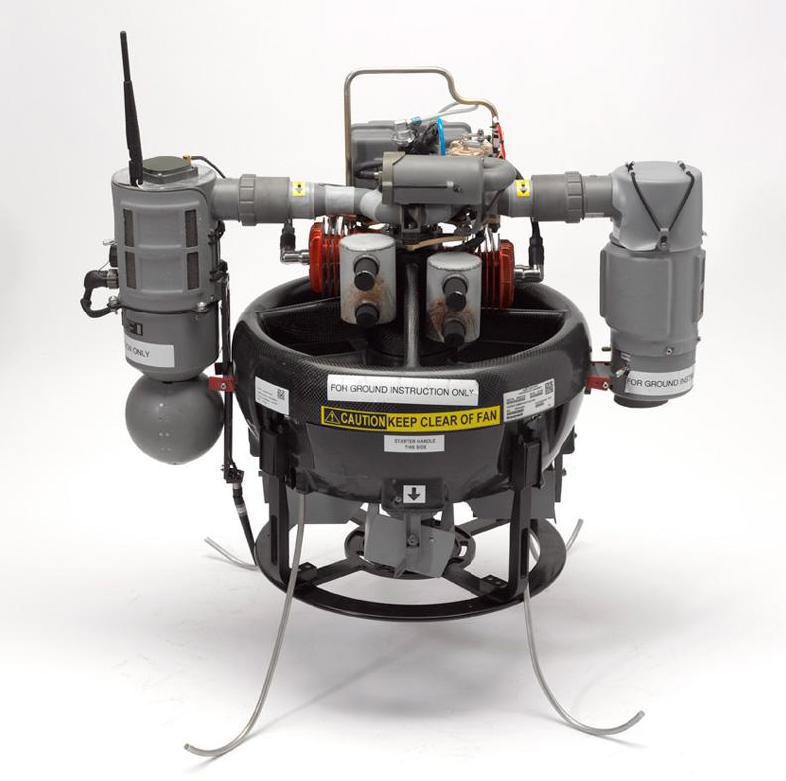
\includegraphics[width=6cm,height=6cm]{Fig/honeywell_t-hawk.jpg}
		\caption{\label{Hawk}T-Hawk}
	\end{minipage}%
	\begin{minipage}[c]{0.5\textwidth}
		\centering
		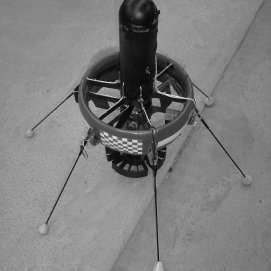
\includegraphics[width=6cm,height=6cm]{Fig/GTSpy.jpg}
		\caption{\label{GTSpy}GTSpy}
	\end{minipage}
\end{figure}
\section{表}
本节仅展示使用常见的三线表
\begin{lstlisting}
\begin{table}
	\caption{\label{TDF_para}涵道模型参数}	%表题在上
	\centering	% 表居中
	\small	% 表内字体小一号(即设置成和表题字号一致)
	\begin{tabular}{cccc}	% cccc表示4列并居中,若列之间需要分隔符则设置为|c|c|c|c|
		\hline	% \hline表示横线。列之间的元素用&分隔,\tabularnewline表示换行
		参数符号 & 数值 & 参数符号 & 数值 \tabularnewline 
		\hline 
		$I_x$ & $054593$ 		   & $I_y$ & $0.017045         $ \tabularnewline
		$l_1$ & $0.0808\,\text{m}$ & $l_2$ & $0.175\,\text{m}  $ \tabularnewline 
		$l_4$ & $0.2415\,\text{m}$ & $l_5$ & $0.1085\,\text{m} $ \tabularnewline
		\hline 
	\end{tabular}
\end{table}
\end{lstlisting}
\begin{table}
	\caption{\label{TDF_para}涵道模型参数}
	\centering
	\small 
	\begin{tabular}{cccc}
		\hline 
		参数符号 & 数值                & 参数符号 & 数值                 \tabularnewline
		\hline 
		$I_x$   & $054593$ 		     & $I_y$   & $0.017045         $ \tabularnewline
		$l_1$   & $0.0808\,\text{m}$ & $l_2$   & $0.175\,\text{m}  $ \tabularnewline 
		$l_4$   & $0.2415\,\text{m}$ & $l_5$   & $0.1085\,\text{m} $ \tabularnewline
		\hline 
	\end{tabular}
\end{table}

\section{公式}
除了前面讲行内公式,常用的还有行间公式。公式中的数学符号可自行百度,本章仅介绍常用的几种公式环境。

单独成行的行间公式在 \LaTeX{} 里由equation 环境包裹。equation 环境为公式自动生成一个编号,这个编号可以用\textbackslash{}label 和\textbackslash{}ref 生成交叉引用,amsmath 宏包的\textbackslash{}eqref 可为引用自动加上圆括号;如式\eqref{eq_1}所示。
\begin{lstlisting}
\begin{equation}
	a+b=c	\label{eq_1}
\end{equation}
\end{lstlisting}
\begin{equation}
	a+b=c	\label{eq_1}
\end{equation}
若不需要编号则加星号,改为
\begin{lstlisting}
\begin{equation*}
	a+b=c
\end{equation*}
\end{lstlisting}
其他环境类似。当使用 \texttt\$ 开启行内公式输入,或是使用{equation} 环境时,\LaTeX\ 就进入了数学模式。
数学模式相比于文本模式有以下特点:
\begin{enumerate}
	\item 数学模式中输入的空格被忽略。数学符号的间距默认由符号的性质(关系符号、运算符等)决定。
	需要人为引入间距时,使用 \textbackslash{}{quad} 和 \textbackslash{}{qquad} 等命令。
	\item {不允许有空行(分段)}。行间公式中也无法用 $ \verb|\\|$命令手动换行。排版多行公式需要用到 其他各种环境。
	\item 所有的字母被当作数学公式中的变量处理,字母间距与文本模式不一致,也无法生成单词之间的空格。
	如果想在数学公式中输入正体的文本,简单情况下可用 \textbackslash{}{mathrm} 命令。
	或者用 {amsmath} 提供的 \textbackslash{}{text} 命令(仅适合在公式中穿插少量文字。如果你的情况正好相反,需要在许多文字中穿插使用公式,则应该像正常的行内公式那样用,而不是滥用 \textbackslash{}{text} 命令)。
\end{enumerate}	

实际上更常用的的是多行公式,不需要对齐的公式组可以使用gather环境,需要对齐的公式组用align 环境。
长公式内可用$ \verb|\\|$ 换行。

如果需要罗列一系列公式,并令其按照等号对齐,可用align 环境,它将公式用\& 隔为两部分并对齐。分隔符通常放在等号左边:
\begin{lstlisting}
\begin{align}
	a & = b + c \\
	& = d + e
\end{align}
\end{lstlisting}
\begin{align}
a & = b + c \\
& = d + e
\end{align}
align 环境会给每行公式都编号。

如果不需要按等号对齐,只需罗列数个公式,可用gather环境:
\begin{lstlisting}
\begin{gather}
	a  = b + c \notag \\
	f = d + e 
\end{gather}
\end{lstlisting}
\begin{gather}
	a  = b + c \notag  \\
	f = d + e 
\end{gather}
gather 环境同样会给每行公式都编号,如果某行不需要编号可在行末用\textbackslash{}notag 仅去掉某行的编号。

align 和gather 有对应的不带编号的版本align* 和gather*。

另一个常见的需求是将多个公式组在一起公用一个编号,编号位于公式的居中位置。为此,
amsmath 宏包提供了诸如aligned、gathered 等环境,与equation 环境套用。以-ed 结尾的
环境用法与前一节不以-ed 结尾的环境用法一一对应。我们仅以aligned 举例:
\begin{lstlisting}
\begin{equation}
	\begin{aligned}
		a &= b + c \\
		d &= e + f + g \\
		h + i &= j + k \\
		l + m &= n
	\end{aligned}
\end{equation}
\end{lstlisting}
\begin{equation}
	\begin{aligned}
		a &= b + c \\
		d &= e + f + g \\
		h + i &= j + k \\
		l + m &= n
	\end{aligned}
\end{equation}
split 环境和aligned 环境用法类似,也用于和equation 环境套用,区别是split 只能
将每行的一个公式分两栏,aligned 允许每行多个公式多栏。

分段函数通常用amsmath 宏包提供的cases 环境,可参考文献\parencite{_c}

amsmath 宏包还直接提供了多种排版矩阵的环境,包括不带定界符的matrix,以及带各种定界符的矩阵pmatrix、bmatrix、Bmatrix、vmatrix、Vmatrix。
其中中括号版的bmatrix最常用。这些矩阵环境需要在公式中使用,比如 align 环境。
\begin{lstlisting}
A= \begin{bmatrix}
		x_{11} & x_{12} & \ldots & x_{1n} \\
		x_{21} & x_{22} & \ldots & x_{2n} \\
		\vdots & \vdots & \ddots & \vdots \\
		x_{n1} & x_{n2} & \ldots & x_{nn}
	\end{bmatrix}
\end{gather}
\end{lstlisting}
\begin{gather}
\bm{A}= \begin{bmatrix}
	x_{11} & x_{12} & \ldots & x_{1n} \\
	x_{21} & x_{22} & \ldots & x_{2n} \\
	\vdots & \vdots & \ddots & \vdots \\
	x_{n1} & x_{n2} & \ldots & x_{nn}
   \end{bmatrix}
\end{gather}	
其中矩阵/向量加粗使用\textbackslash{}bm\{\}命令。另外还可以使用array环境排版矩阵,类似tabular环境,用$ \verb|\\|$ 和\& 用来分隔行和列,这里不再赘述。	
\begin{lstlisting}
\begin{array }[外部对齐tcb]{列对齐lcr}
	行列内容
\end{array}
\end{lstlisting}

另外注意排版分式时,有两种方法:\textbackslash{}frac或者\textbackslash{}dfrac,效果分别为$ \frac{1}{2} $和$ \dfrac{1}{2} $。以上介绍的数学环境中,空格可参考文献\parencite{_c},例如常用\textbackslash{}quad。
\section{定理}
在scutthesis.cls文件536行开始,已经用\textbackslash{}newtheorem命令定义了几种定理环境,包括:定义、假设、定理、结论、引理、公理、推论、性质等等,统称定理环境,关于\textbackslash{}newtheorem的用法,可参考\cite{_c}或自行百度。要下面提供几个例子,在横线之间的深色区域是代码,效果在相应下方表示:
\begin{lstlisting}
\begin{assumption}
	加权矩阵${{\bm{W}}_{1}}$和 ${{\bm{W}}_{2}}$ 是对称矩阵,且$ {{\bm{W}}_{2}}$非奇异。	\label{assum_dca1}
\end{assumption}
\end{lstlisting}
\begin{assumption}
	加权矩阵${{\bm{W}}_{1}}$和 ${{\bm{W}}_{2}}$ 是对称矩阵,且$ {{\bm{W}}_{2}}$非奇异。	\label{assum_dca1}
\end{assumption}

定理用法和假设类似:
\begin{lstlisting}
\begin{theorem}
	如果假设\ref{assum_dca1}成立,$\bm{F}$满足式\eqref{eq_F}的定义,且${{\bm{W}}_{1}}$非奇异,则有$0\le e \left( \bm{F} \right) < 1$,其中$e \left( \bm{F} \right)$是 $\bm{F}$的特征值。	\label{the_dca2}
\end{theorem}
\end{lstlisting}
\begin{theorem}
	如果假设\ref{assum_dca1}成立,$\bm{F}$满足上式的定义,且${{\bm{W}}_{1}}$非奇异,则有$0\le e \left( \bm{F} \right) < 1$,其中$e \left( \bm{F} \right)$是 $\bm{F}$的特征值。	\label{the_dca2}
\end{theorem}

定理环境的编号可自定义,但通常不需要再进行设置,因为模板文件scutthesis.cls文件已经定义好。
\section{参考文献}

\begin{lstlisting}
关于参考文献这块,很多同学有疑问。只有记住一点:不管用什么参考文献管理工具,最终目的是生成一个bib文件给TeXstudio使用,bib文件里是特定格式的文献信息。bib文件可以使用一个叫notepad++的软件打开。
\end{lstlisting}

通常学位论文参考文献是基于BibTeX进行的,本模板最大的改进就是引入BibLaTeX。关于这部分知识可参考文献\parencite{_c,_g}的第六章,6.1节参考文献和BIBTEX工具。

参考文献引用和著录是基于ZOTERO这个软件进行的。视频教程见\parencite{_k}。此外,为了符合毕业论文撰写规范,需设置参数。按照视频教程安装完必要的插件(如Better BibTeX)后,在编辑->首选项进行设置。附录图\ref{op1}到图\ref{op11}所示的是我的zotero软件设置。其中最重要的是\ref{op10}的设置要排除的选项,多余的显示会让审稿人反感,按照论文撰写规范进行即可。在毕业论文撰写时,在编辑->首选项->Better BibLTeX->Fields中,Fields to omit from export填month,abstract,note,extra,file,keywords,type,url,doi,就是在参考文献著录中排除这些多余的项,避免过于复杂。而在写本模板使用说明时,没有排除url,因为很多参考资料是网页。

\begin{lstlisting}
使用zotero,科学上网很重要,通常我们使用谷歌学术搜索文献并利用chrome的zotero插件直接捕获文献著录信息。但我使用蓝灯,代理服务器均遇到过被谷歌学术封锁的情况。只能不断换科学上网方法。这里我现在用的chrome插件:谷歌上网助手,它可以轻松捕获谷歌学术的著录信息,注册一个账号即可使用。谷歌上网助手有可能和某些代理冲突。这些都是科学上网的问题,已经超出了本项目的范围,听说百度一下 v2ray 可发现新大陆,可惜我试了Vultr的服务器依然被谷歌封。知网捕获中文参考文献著录信息的话不需要考虑这个问题,直接在知网首页搜索文献然后点击插件既可以选想捕获的著录了。
\end{lstlisting}

在zotero软件点击文件->导出文献库,如图\ref{output}所示,再在导出对话框图\ref{output_format}选择导出格式为Better BibLaTeX,同时勾选Keep updated选项保持自动更新,再点击ok,在弹出的对话框图\ref{output_name}确定保存路径和文件名,例如我的是MyLibrary.bib,这也是我整个读书生涯的文献库bib文件。如果写小论文的话通常导出格式是BibTeX或者Better BibTeX(这里按照期刊的要求来即可,文献管理软件的好处就是快速自动生成一个文件库)。关于BibTeX和BibLaTeX的区别这里不做展开。

得到文献库后,在scutthesis.tex文件第九行使用\textbackslash{}addbibresource命令,添加文献库。引用某文献时秩序在zotero选中某文献条目,然后按Ctrl+Shift+C,复制引用关键字(Citation Key)到剪切板(快捷键可自定义)。然后在tex文件编辑界面直接粘贴,默认的时上标形式,若需要非上标形式,可以改为\textbackslash{}parencite{XXXX},其中XXXX是Citation Key。这里的操作和认为设置的首选项参数有关,需要在编辑->首选项->导出界面的默认格式一栏选中相应的项,同时在编辑->首选项->高级->快捷键设置为默认值。

---------------------------------------------------------------------------------

2020年12月2日测试:
下载最新zotero,从知网和谷歌捕获文献(刚打开网页最好稍等一会再点击插件,谷歌可能需要现人机验证),对文献\parencite{Renduchintala_2019}、\parencite{Meng_2020}进行引用。

---------------------------------------------------------------------------------
\begin{lstlisting}
另外有同学反映,换了电脑后重新导出的bib文件Citation Key值不同,记得设置好Better BibTeX之后,在著录条目界面全选著录(或仅选想更新的著录)然后右键选Better BibTeX更新refresh一下。然后在Automatic export选项点击Export now立即更新bib文件(按理说勾选了自动更新选项他会自动更新,但为了确保万无一失还是点一下)。
\end{lstlisting}










 % 第三章
% 自行根据需要添加章节。
...
\chapter{结\texorpdfstring{\quad}{}论}
本文主要是展示如何使用修改“祖传模板”得到的新模板,在使用时直接替换成自己的论文内容即可。总结下来最最最麻烦的是科学上网,只有科学上网才能获取文献信息生成bib文件,后面就好办了。

本模板难免有不足之处,主要是我本人的论文涉及的格式有限,有些地方没探索到自然就没去设置。比如附录,附录的图文并茂等等,我本人是没有研究的,这里仅仅做了一些初步的工作,不过对很多同学来说本模板是够用的。希望有能帮助到华工的同学们,有不足之处请多多理解,可以通过邮件联系我,上班之余我会尽量回复。 % 结论
...
\printbibliography	% 参考文献著录
\chapter{附\texorpdfstring{\quad}{}录}
\renewcommand{\thesection}{{附录}\arabic{section}}
\setcounter{section}{0}
\section{zotero的设置}
\begin{figure}
	\centering
	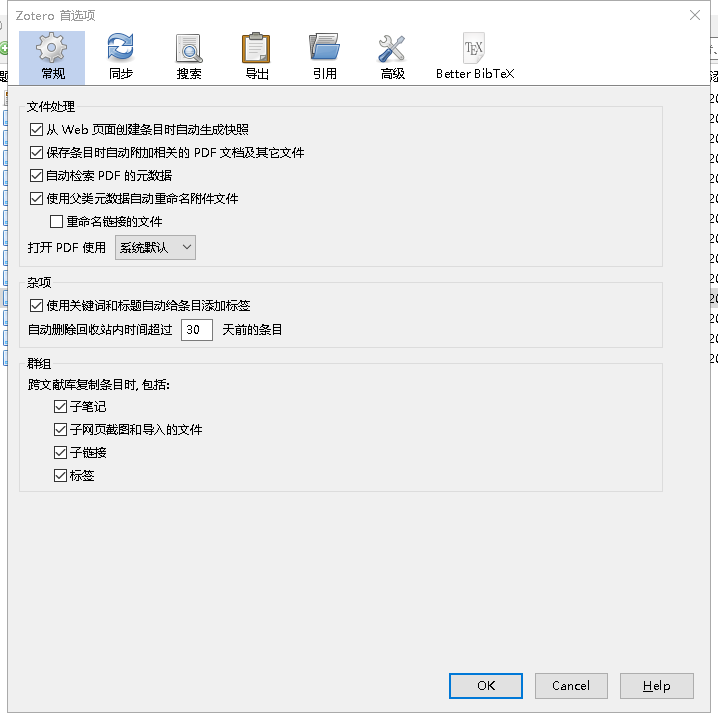
\includegraphics[scale=0.8]{Fig/zotero1.png}
	\caption{\label{op1}常规}
\end{figure}
\begin{figure}
	\centering
	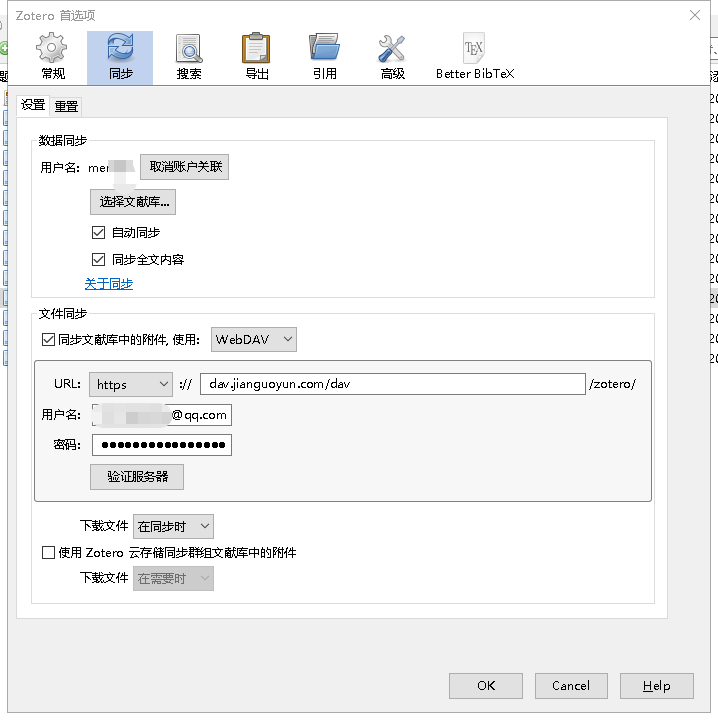
\includegraphics[scale=0.8]{Fig/zotero2.png}
	\caption{\label{op2}同步1}
\end{figure}
\begin{figure}
	\centering
	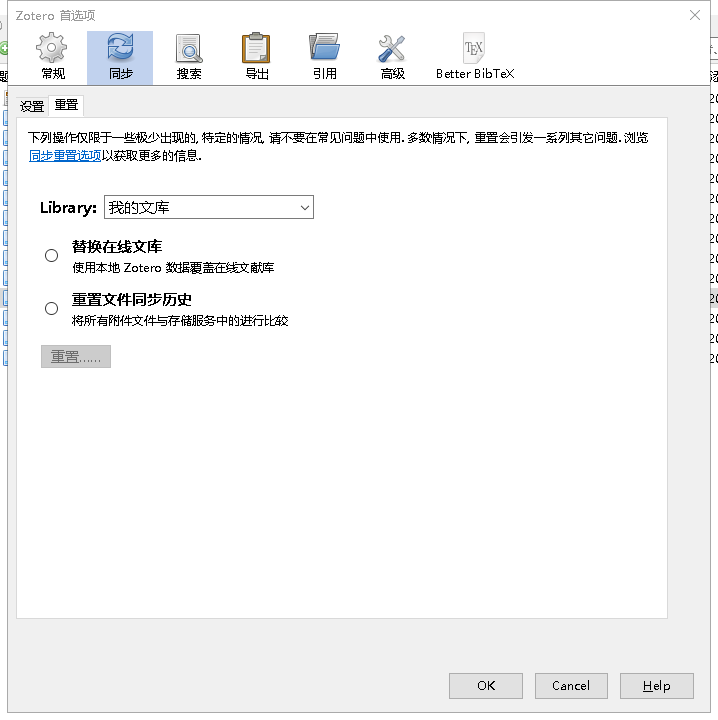
\includegraphics[scale=0.8]{Fig/zotero3.png}
	\caption{\label{op3}同步2}
\end{figure}
\begin{figure}
	\centering
	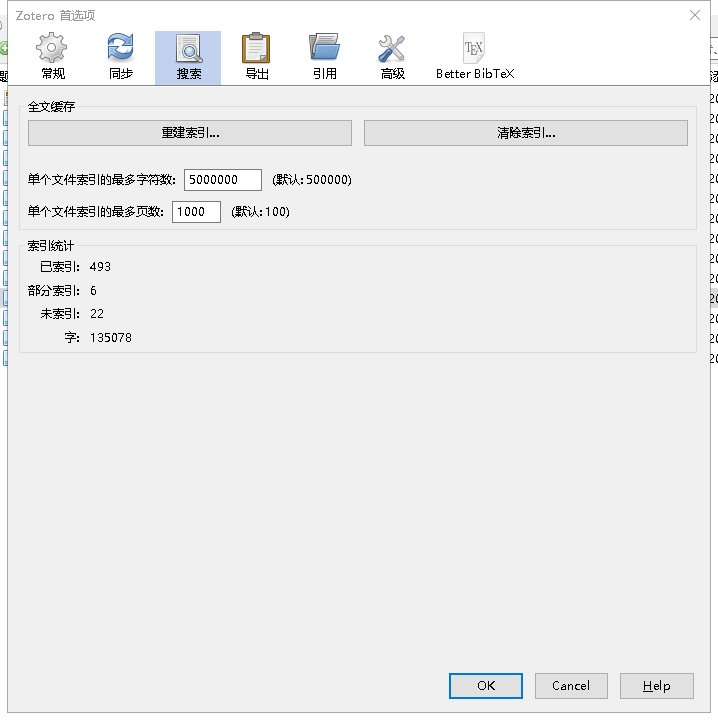
\includegraphics[scale=0.8]{Fig/zotero4.png}
	\caption{\label{op4}搜索}
\end{figure}
\begin{figure}
	\centering
	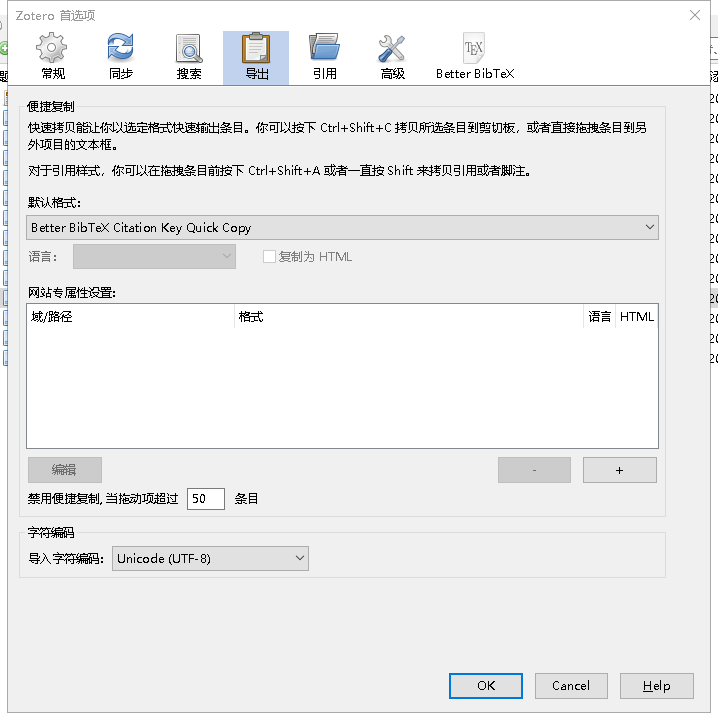
\includegraphics[scale=0.8]{Fig/zotero5.png}
	\caption{\label{op5}导出}
\end{figure}
\begin{figure}
	\centering
	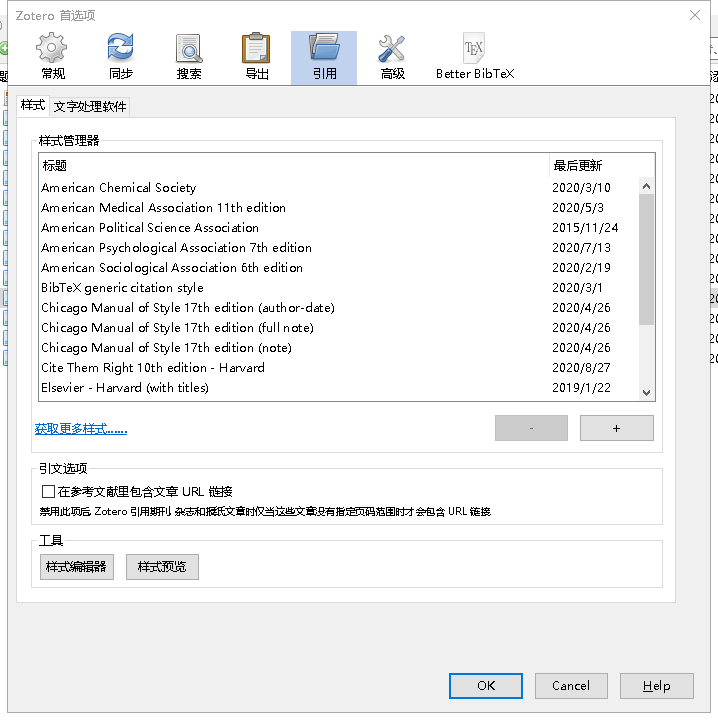
\includegraphics[scale=0.8]{Fig/zotero6.png}
	\caption{\label{op6}引用}
\end{figure}
\begin{figure}
	\centering
	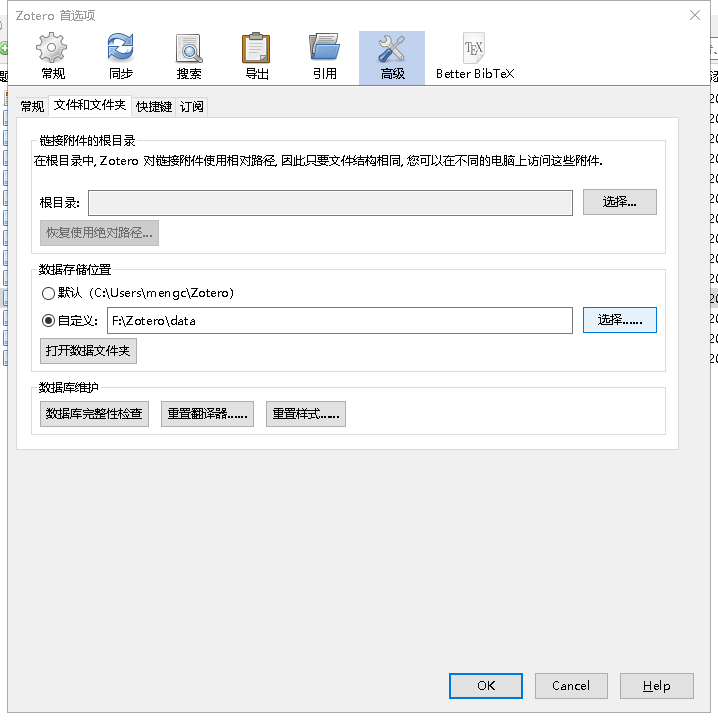
\includegraphics[scale=0.8]{Fig/zotero7.png}
	\caption{\label{op7}高级1}
\end{figure}
\begin{figure}
	\centering
	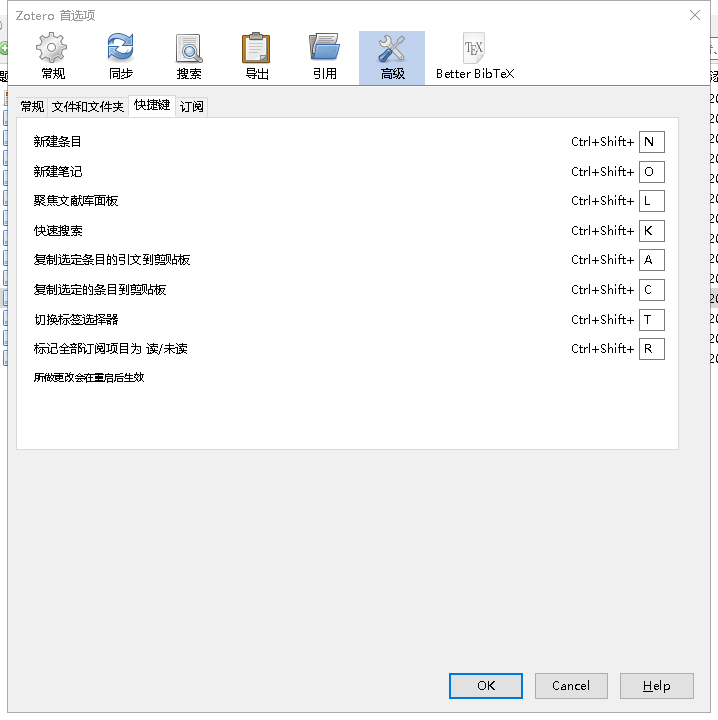
\includegraphics[scale=0.8]{Fig/zotero8.png}
	\caption{\label{op8}高级2}
\end{figure}
\begin{figure}
	\centering
	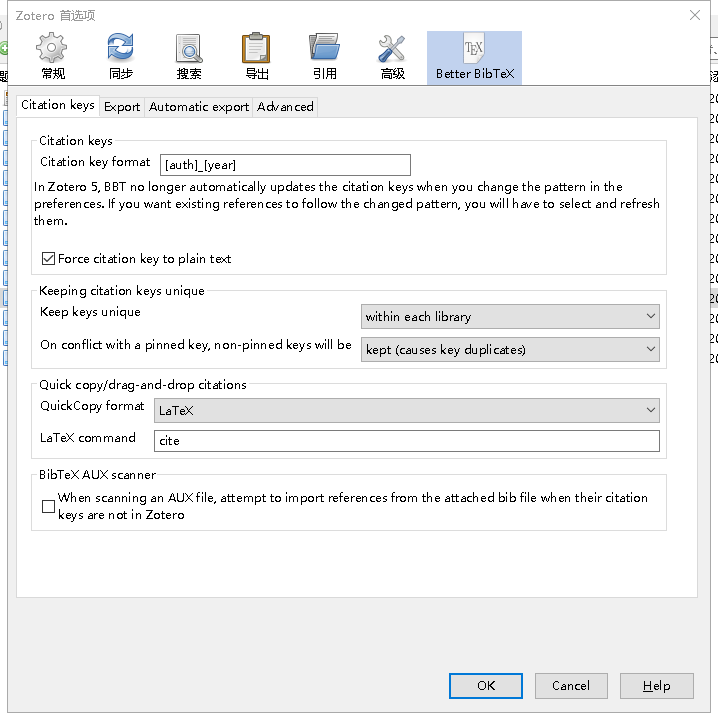
\includegraphics[scale=0.8]{Fig/zotero9.png}
	\caption{\label{op9}Better BibTeX1}
\end{figure}
\begin{figure}
	\centering
	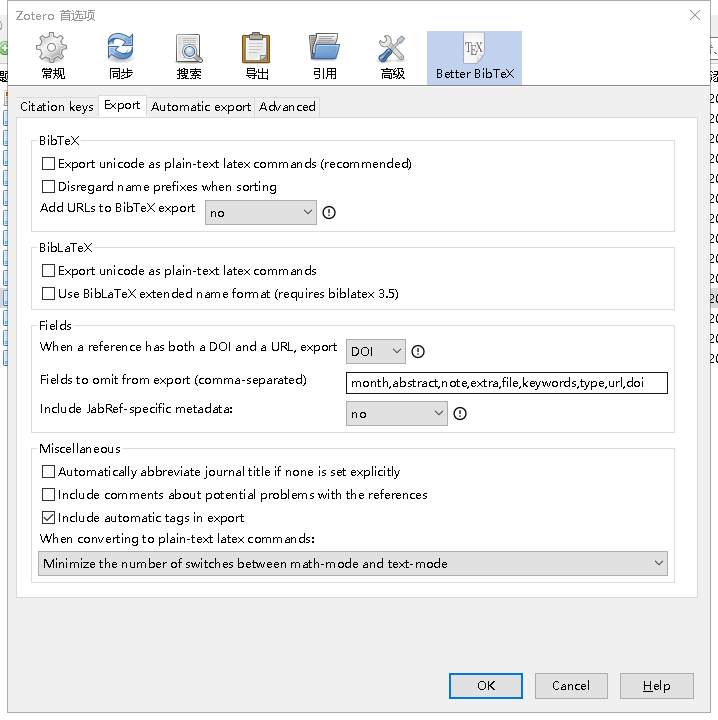
\includegraphics[scale=0.8]{Fig/zotero10.png}
	\caption{\label{op10}Better BibTeX2}
\end{figure}
\begin{figure}
	\centering
	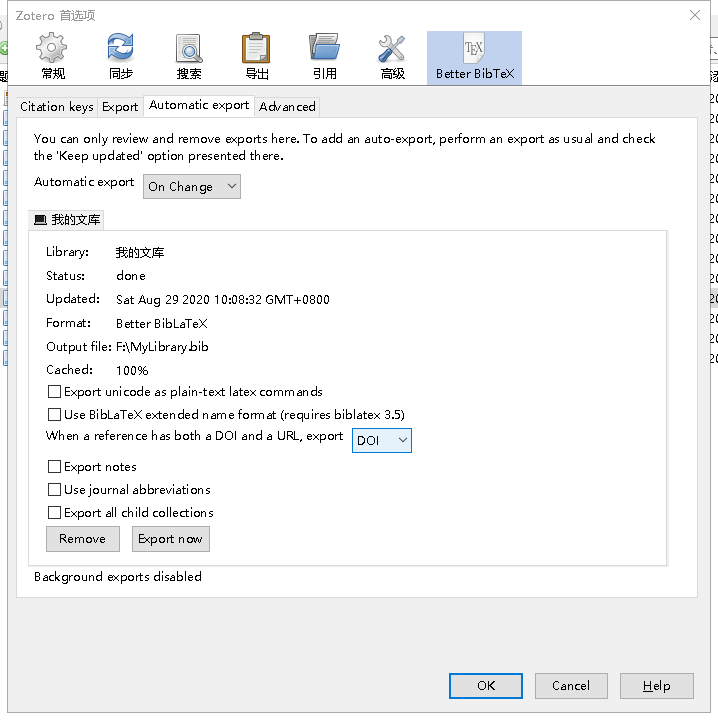
\includegraphics[scale=0.8]{Fig/zotero11.png}
	\caption{\label{op11}Better BibTeX3}
\end{figure}

\begin{figure}[htbp]
	\centering
	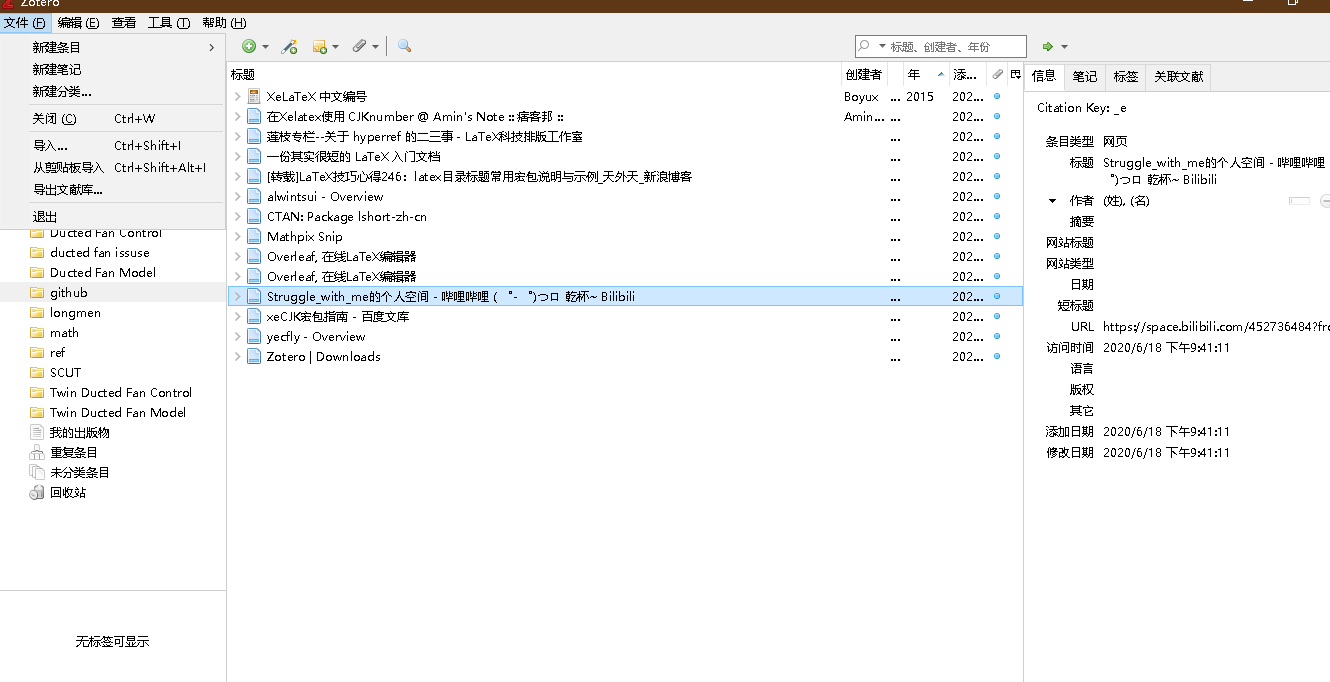
\includegraphics[scale=0.42]{Fig/zotero12.png}
	\caption{\label{output}导出文献库}
\end{figure}

\begin{figure}[htbp]
	\centering
	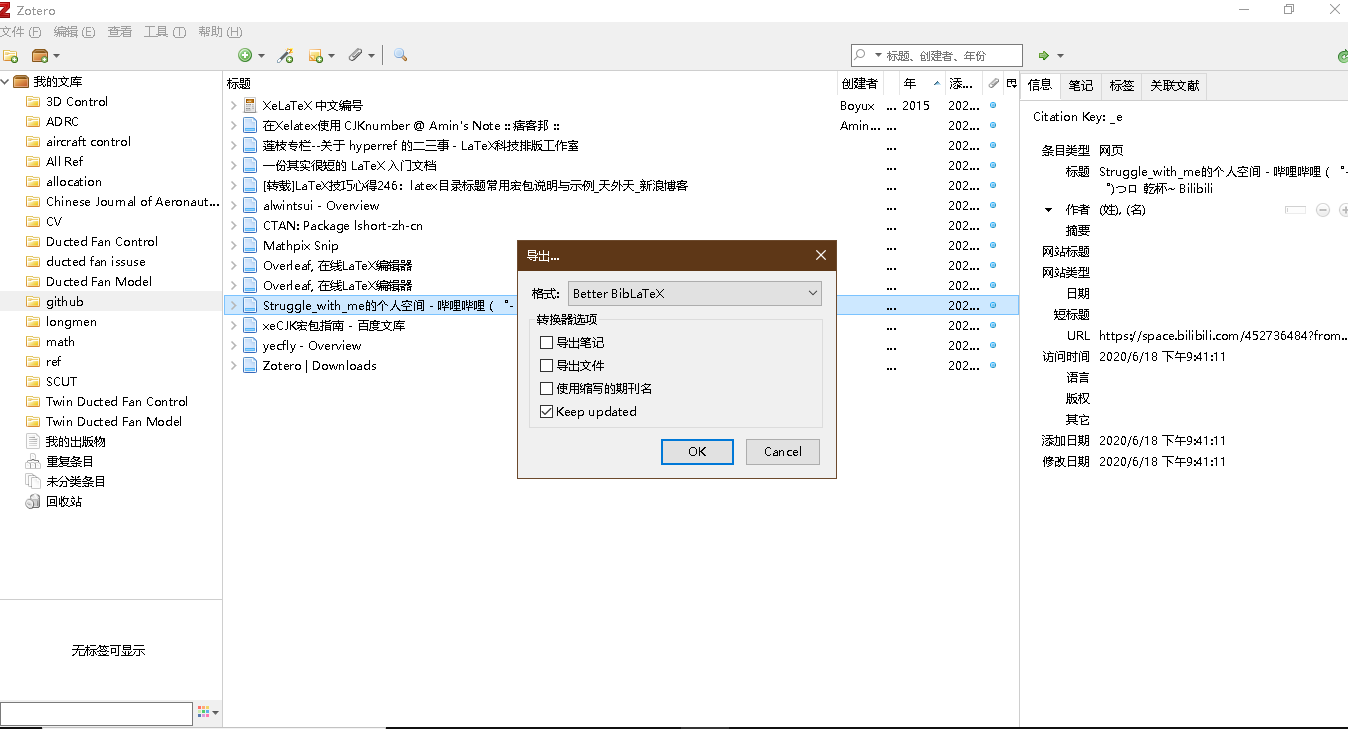
\includegraphics[scale=0.42]{Fig/zotero13.png}
	\caption{\label{output_format}导出格式}
\end{figure}

\begin{figure}[htbp]
	\centering
	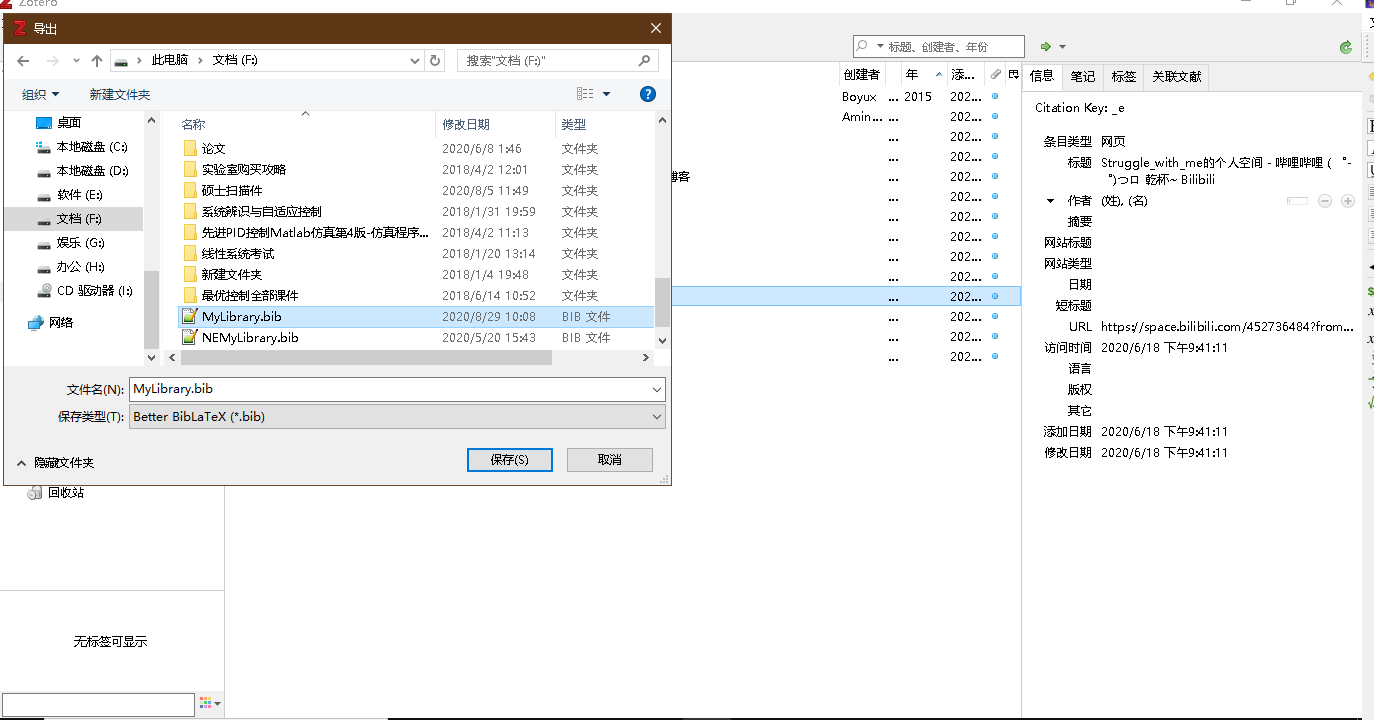
\includegraphics[scale=0.42]{Fig/zotero14.png}
	\caption{\label{output_name}导出文件名}
\end{figure}
\section{BibLatex}

 % 附录
\chapter{攻读硕士学位期间取得的研究成果}
已发表(包括已接受待发表)的论文,以及已投稿、或已成文打算投稿、或拟成文投稿的论文情况(只填写与学位论文内容相关的部分):
\begin{table}
	\centering{}%
	\small 
	\begin{longtable}{|>{\centering}m{0.5cm}|m{1.8cm}|>{\centering}m{2.8cm}|>{\centering}m{2.5cm}|>{\centering}m{2.2cm}|>{\centering}m{2.cm}|>{\centering}m{1cm}|}
		\hline 
		序号 & 作者(全体作者,按顺序排列) & 题 目 						   & 发表或投稿刊物名称、级别 & 发表的卷期、年月、页码 & 相当于学位论文的哪一部分(章、节) & 被索引收录情况\tabularnewline
		\hline 
		1    & 蒙超恒、裴海龙、程子欢					  & 涵道风扇式无人机的优先级控制分配 & 航空学报 & 已录用,2020年5月 & 2.1、2.2、3.4、4.1、4.2、5.1和5.3节 & EI\tabularnewline
		\hline 
		2	 & 	蒙超恒、裴海龙、程子欢						&  	Dynamic Control Allocation for A Twin Ducted Fan UAV							 & 2020 International Conference on Guidance, Navigation and Control  & 已录用,2020年8月 & 2.3、4.3和5.2节 &EI \tabularnewline
		\hline 
	\end{longtable}
\end{table}

注:在“发表的卷期、年月、页码”栏:

1.如果论文已发表,请填写发表的卷期、年月、页码;

2.如果论文已被接受,填写将要发表的卷期、年月;

3.以上都不是,请据实填写“已投稿”,“拟投稿”。

不够请另加页。

二、与学位内容相关的其它成果(包括专利、著作、获奖项目等)



%注:这部分一言难尽,我努力了很久都没有把这个表做好。感觉学校给的这个表的模板非常反人类。看国外大学的博士论文,那种像参考文献著录信息那样一行一行的,比较美观。而这个框框很难放文字进去。 % 成果
\chapter{致\texorpdfstring{\quad}{}谢}
%把下面文字替换
\begin{center}
这次你离开了没有像以前那样说再见,再见也他妈的只是再见 
~\\
我们之间从来没有想象的那么接近,只是两棵树的距离 
~\\
你是否还记得山阴路我八楼的房间,房间里唱歌的日日夜夜 
~\\
那么热的夏天你看着外面,看着你在消逝的容颜 
~\\
我多么想念你走在我身边的样子,想起来我的爱就不能停止 
~\\
南京的雨不停地下不停地下,就像你沉默的委屈 
~\\
一转眼,我们的城市又到了夏天,对面走来的人都眯着眼 
~\\
人们不敢说话不敢停下脚步,因为心动常常带来危险 
~\\
我多么想念你走在我身边的样子,想起来我的爱就不能停止 
~\\
南京的雨不停地下不停地下,有些人却注定要相遇 
~\\
你是一片光荣的叶子,落在我卑贱的心 
~\\
像往常一样我为自己生气并且歌唱 
~\\
那么乏力,爱也吹不动的叶子 
\end{center}
%把上面文字替换

~\\

\begin{minipage}[t]{0.945\textwidth}%
	\begin{flushright}
		蒙超恒\\
		\today\\	% 时间
		于华南理工大学
		\par\end{flushright}
\end{minipage}

 % 致谢
\end{lstlisting}
其中$\%$之后的内容为注释,...表示省略其他代码,仅保留论文内容主体部分。\textbackslash{}include\{xxx\}指令用于包含xxx.tex文件的内容,各章节的内容主要在xxx.tex中保存。在\textbackslash{}documentclass 和\textbackslash{}begin\{document\} 之间的位置称为导言区。在导言区中一般会使用\textbackslash{}usepackage 调用宏包,以及会进行对文档的全局设置。本模板的导言区除调用所需的宏包外,还进行了页眉页脚的设置。有的模板会把所有调用宏包的指令放到一个.sty宏包文件中,页面的设置放在文档类文件.cls文件中。因本人时间有限,就不做整理,欢迎有志之士加入完善。使用本模板并不需要了解导言区的指令,在需要时额外添加即可(要注意宏包冲突)。特别地,\textbackslash{}includeonly\{xxx\}指令用于使文档仅编译xxx.tex文件的内容,这就是分章节包含(include)的好处,可大大减少编译时间。

将封面打印保存为 thesis\_cover.pdf 文件,硕士使用master\_cover.docx ,博士使用 doctor\_cover.doc 。如果有更新版本的封面,可自行替换。文档类默认是博士论文,下面指令将控制添加封面与否:
\begin{lstlisting}
\documentclass[unicode,master,pdfcover]{scutthesis}	% 使用pdf文件封面的 硕士模板
\documentclass[unicode,master]{scutthesis}	% 不使用pdf文件封面的 硕士模板
\documentclass[unicode,pdfcover]{scutthesis}	% 使用pdf文件封面的博士模板
\documentclass[unicode]{scutthesis}	% 不使用pdf文件封面的博士模板
\end{lstlisting}
不使用thesis\_cover.pdf 文件指定的封面时,将使用草稿封面。草稿封面也可以减少编译时间,因此可以在最终提交论文时再使用论文封面。草稿封面用以下指令设置:
\begin{lstlisting}
%%%%%%%%%%%%%草稿封面设置%%%%%%%%%%%%%	
\title{LaTeX模板}	
\author{蒙超恒}	
\supervisor{指导教师:裴海龙\ 教授}	
\institute{华南理工大学}	
\date{2020年5月20日}
%%%%%%%%%%%%%%%%%%%%%%%%%%%%%%%%%%%%%
\end{lstlisting}
\section{章节文件}
章节文件如chapter0x.tex等,其内容由\textbackslash{}chapter\{章名\}开头。新建一章可新建一个文件并由\textbackslash{}chapter\{新建章名\}开头填写内容即可。节及小节分别用\textbackslash{}section\{新建节名\}、\textbackslash{}subsection\{新建小节名\}命令。

正文的的书写和txt文本文件的书写类似。\LaTeX{} 源代码中,空格键和Tab键输入的空白字符视为“空格”。连续的若干个空白字符视为一个空格。一行开头的空格忽略不计。行末的回车视为一个空格;但连续两个回车,也就是空行,会将文字分段。多个空行被视为一个空行。也可以在行末使用\textbackslash{}par 命令分段。在本模板中,英文之间的空格被保留,中文之间的空格被忽略。特别地,摘要,附录,结论等两个字的大纲级别为章的章名,中间使用空格隔开。对此论文撰写规范并没有明文要求,只是为了美观。也可以全部不加空格。一般情况下,在文本文字中添加空格使用\textbackslash{}quad命令,但由于文献\parencite{_d}所述原因,直接使用\textbackslash{}quad命令会报警,因而使用\textbackslash{}texorpdfstring\{\textbackslash{}quad\}\{\},其中最后一个\{\}里面可以加一个空格,不影响使用。目录二字之间添加空格在scutthesis.cls文件317行设置。

正文本环境中使用公式,即行内公式,需要用两个\$包围,如源码:\$a+b=c\$ 显示为$a+b=c$。使用其他字符可自行百度或阅读参考文献。再次提醒,使用\LaTeX{}撰写论文不需要研究其原理,在达到某种效果(图文显示、公式显示效果)时百度或查书寻找其代码即可。

综上,论文撰写只需要将自己的文本(包含行内公式)放到相应的章节处,并添加行间公式、图表环境并填写图表即可。行间公式、图表将在下一章介绍。

%第二章
	
\chapter{常用环境及参考文献设置}
强烈建议在使用公式、表格、定理环境时进行百度,没必要研究各种用法,只需要知道自己需要什么。因本人的论文所用表格较少,因而对表格不是很熟悉,本章对表格的介绍相应的较少。本章仅介绍本人在论文撰写过程中常用的环境以及参考文献设置。

\section{图}
图的导入需要提前准备好图片文件,最好是.png、.eps、.pdf或.jpg文件。另外,如果是从matlab导出图片文件,可使用print函数或手动导出,print函数的使用可参考ICGNC2020plot.m以及PlotToFileColorPDF.m文件等。手动导出(matlab的figure界面的“文件”->“导出设置”设置好大小分辨率和线宽等然后点击“应用于图窗”)主要用于观察效果,可设置某种导出样式后导出该样式,下次使用时加载,具体可百度“matlab导出高清图片”。需要特别注意的是一定要1:1导入matlab生成的图片,并且图中文字设置好字体字号。

使用如下代码放置独立成行的图片,效果如图\ref{one_DFUAV}所示
\begin{lstlisting}
\begin{figure}[htbp]
	% 图片居中(列居中对齐)
	\centering	
	% 包含当前路径下的Fig文件夹的图片文件DFUAV_f31.png
	\includegraphics[scale=1]{Fig/DFUAV_f31.png} 
	% 添加标签one_DFUAV以及图标题“涵道风扇式无人机”,标题编号是自动生成的
	\caption{\label{one_DFUAV}涵道风扇式无人机} 
\end{figure}
\end{lstlisting}
其中figure为环境名,[htbp]表示将图片设置为浮动体,实际上这在.cls文件已经设置过,因而可以省略。[scale=1]表示安装1:1的比例导入图片,还可以按其他方式导入,需要时可自行百度。
\begin{figure}[htbp]
	\centering
	\includegraphics[scale=1]{Fig/DFUAV_f31.png}
	\caption{\label{one_DFUAV}涵道风扇式无人机}
\end{figure}

使用如下代码划分页面并排放置图\ref{Hawk}、图\ref{GTSpy}
\begin{lstlisting}
\begin{figure}[htbp]
	\centering
	\begin{minipage}[c]{0.5\textwidth} % minipage将页面划分为0.5\textwidth
		\centering
		\includegraphics[width=6cm,height=6cm]{Fig/honeywell_t-hawk.jpg}
		\caption{\label{Hawk}T-Hawk}
	\end{minipage}%
	\begin{minipage}[c]{0.5\textwidth}
		\centering
		\includegraphics[width=6cm,height=6cm]{Fig/GTSpy.jpg}
		\caption{\label{GTSpy}GTSpy}
	\end{minipage}
\end{figure}
\end{lstlisting}
其中[c]表示行居中对齐。当图片大小不一但又需要1:1导入时,图标题可能行不对齐,因此可以改为如下指令:
\begin{lstlisting}
\begin{figure}[htbp]
	\centering
	\begin{minipage}[c]{0.5\textwidth}
		\centering
		\includegraphics[scale=1]{Fig/honeywell_t-hawk.jpg} %1:1导入
	\end{minipage}%
	\begin{minipage}[c]{0.5\textwidth}
		\centering
		\includegraphics[scale=1]{Fig/GTSpy.jpg}
	\end{minipage}\\[1pt]
	\begin{minipage}[t]{0.5\textwidth}	% 以下为新添加页面划分,[t]表示行顶部对齐
		\caption{\label{Hawk}T-Hawk}
	\end{minipage}%
	\begin{minipage}[t]{0.5\textwidth}
		\caption{\label{GTSpy}GTSpy}
	\end{minipage}%
\end{figure}
\end{lstlisting}
\begin{figure}[htbp]
	\centering
	\begin{minipage}[c]{0.5\textwidth}
		\centering
		\includegraphics[width=6cm,height=6cm]{Fig/honeywell_t-hawk.jpg}
		\caption{\label{Hawk}T-Hawk}
	\end{minipage}%
	\begin{minipage}[c]{0.5\textwidth}
		\centering
		\includegraphics[width=6cm,height=6cm]{Fig/GTSpy.jpg}
		\caption{\label{GTSpy}GTSpy}
	\end{minipage}
\end{figure}
\section{表}
本节仅展示使用常见的三线表
\begin{lstlisting}
\begin{table}
	\caption{\label{TDF_para}涵道模型参数}	%表题在上
	\centering	% 表居中
	\small	% 表内字体小一号(即设置成和表题字号一致)
	\begin{tabular}{cccc}	% cccc表示4列并居中,若列之间需要分隔符则设置为|c|c|c|c|
		\hline	% \hline表示横线。列之间的元素用&分隔,\tabularnewline表示换行
		参数符号 & 数值 & 参数符号 & 数值 \tabularnewline 
		\hline 
		$I_x$ & $054593$ 		   & $I_y$ & $0.017045         $ \tabularnewline
		$l_1$ & $0.0808\,\text{m}$ & $l_2$ & $0.175\,\text{m}  $ \tabularnewline 
		$l_4$ & $0.2415\,\text{m}$ & $l_5$ & $0.1085\,\text{m} $ \tabularnewline
		\hline 
	\end{tabular}
\end{table}
\end{lstlisting}
\begin{table}
	\caption{\label{TDF_para}涵道模型参数}
	\centering
	\small 
	\begin{tabular}{cccc}
		\hline 
		参数符号 & 数值                & 参数符号 & 数值                 \tabularnewline
		\hline 
		$I_x$   & $054593$ 		     & $I_y$   & $0.017045         $ \tabularnewline
		$l_1$   & $0.0808\,\text{m}$ & $l_2$   & $0.175\,\text{m}  $ \tabularnewline 
		$l_4$   & $0.2415\,\text{m}$ & $l_5$   & $0.1085\,\text{m} $ \tabularnewline
		\hline 
	\end{tabular}
\end{table}

\section{公式}
除了前面讲行内公式,常用的还有行间公式。公式中的数学符号可自行百度,本章仅介绍常用的几种公式环境。

单独成行的行间公式在 \LaTeX{} 里由equation 环境包裹。equation 环境为公式自动生成一个编号,这个编号可以用\textbackslash{}label 和\textbackslash{}ref 生成交叉引用,amsmath 宏包的\textbackslash{}eqref 可为引用自动加上圆括号;如式\eqref{eq_1}所示。
\begin{lstlisting}
\begin{equation}
	a+b=c	\label{eq_1}
\end{equation}
\end{lstlisting}
\begin{equation}
	a+b=c	\label{eq_1}
\end{equation}
若不需要编号则加星号,改为
\begin{lstlisting}
\begin{equation*}
	a+b=c
\end{equation*}
\end{lstlisting}
其他环境类似。当使用 \texttt\$ 开启行内公式输入,或是使用{equation} 环境时,\LaTeX\ 就进入了数学模式。
数学模式相比于文本模式有以下特点:
\begin{enumerate}
	\item 数学模式中输入的空格被忽略。数学符号的间距默认由符号的性质(关系符号、运算符等)决定。
	需要人为引入间距时,使用 \textbackslash{}{quad} 和 \textbackslash{}{qquad} 等命令。
	\item {不允许有空行(分段)}。行间公式中也无法用 $ \verb|\\|$命令手动换行。排版多行公式需要用到 其他各种环境。
	\item 所有的字母被当作数学公式中的变量处理,字母间距与文本模式不一致,也无法生成单词之间的空格。
	如果想在数学公式中输入正体的文本,简单情况下可用 \textbackslash{}{mathrm} 命令。
	或者用 {amsmath} 提供的 \textbackslash{}{text} 命令(仅适合在公式中穿插少量文字。如果你的情况正好相反,需要在许多文字中穿插使用公式,则应该像正常的行内公式那样用,而不是滥用 \textbackslash{}{text} 命令)。
\end{enumerate}	

实际上更常用的的是多行公式,不需要对齐的公式组可以使用gather环境,需要对齐的公式组用align 环境。
长公式内可用$ \verb|\\|$ 换行。

如果需要罗列一系列公式,并令其按照等号对齐,可用align 环境,它将公式用\& 隔为两部分并对齐。分隔符通常放在等号左边:
\begin{lstlisting}
\begin{align}
	a & = b + c \\
	& = d + e
\end{align}
\end{lstlisting}
\begin{align}
a & = b + c \\
& = d + e
\end{align}
align 环境会给每行公式都编号。

如果不需要按等号对齐,只需罗列数个公式,可用gather环境:
\begin{lstlisting}
\begin{gather}
	a  = b + c \notag \\
	f = d + e 
\end{gather}
\end{lstlisting}
\begin{gather}
	a  = b + c \notag  \\
	f = d + e 
\end{gather}
gather 环境同样会给每行公式都编号,如果某行不需要编号可在行末用\textbackslash{}notag 仅去掉某行的编号。

align 和gather 有对应的不带编号的版本align* 和gather*。

另一个常见的需求是将多个公式组在一起公用一个编号,编号位于公式的居中位置。为此,
amsmath 宏包提供了诸如aligned、gathered 等环境,与equation 环境套用。以-ed 结尾的
环境用法与前一节不以-ed 结尾的环境用法一一对应。我们仅以aligned 举例:
\begin{lstlisting}
\begin{equation}
	\begin{aligned}
		a &= b + c \\
		d &= e + f + g \\
		h + i &= j + k \\
		l + m &= n
	\end{aligned}
\end{equation}
\end{lstlisting}
\begin{equation}
	\begin{aligned}
		a &= b + c \\
		d &= e + f + g \\
		h + i &= j + k \\
		l + m &= n
	\end{aligned}
\end{equation}
split 环境和aligned 环境用法类似,也用于和equation 环境套用,区别是split 只能
将每行的一个公式分两栏,aligned 允许每行多个公式多栏。

分段函数通常用amsmath 宏包提供的cases 环境,可参考文献\parencite{_c}

amsmath 宏包还直接提供了多种排版矩阵的环境,包括不带定界符的matrix,以及带各种定界符的矩阵pmatrix、bmatrix、Bmatrix、vmatrix、Vmatrix。
其中中括号版的bmatrix最常用。这些矩阵环境需要在公式中使用,比如 align 环境。
\begin{lstlisting}
A= \begin{bmatrix}
		x_{11} & x_{12} & \ldots & x_{1n} \\
		x_{21} & x_{22} & \ldots & x_{2n} \\
		\vdots & \vdots & \ddots & \vdots \\
		x_{n1} & x_{n2} & \ldots & x_{nn}
	\end{bmatrix}
\end{gather}
\end{lstlisting}
\begin{gather}
\bm{A}= \begin{bmatrix}
	x_{11} & x_{12} & \ldots & x_{1n} \\
	x_{21} & x_{22} & \ldots & x_{2n} \\
	\vdots & \vdots & \ddots & \vdots \\
	x_{n1} & x_{n2} & \ldots & x_{nn}
   \end{bmatrix}
\end{gather}	
其中矩阵/向量加粗使用\textbackslash{}bm\{\}命令。另外还可以使用array环境排版矩阵,类似tabular环境,用$ \verb|\\|$ 和\& 用来分隔行和列,这里不再赘述。	
\begin{lstlisting}
\begin{array }[外部对齐tcb]{列对齐lcr}
	行列内容
\end{array}
\end{lstlisting}

另外注意排版分式时,有两种方法:\textbackslash{}frac或者\textbackslash{}dfrac,效果分别为$ \frac{1}{2} $和$ \dfrac{1}{2} $。以上介绍的数学环境中,空格可参考文献\parencite{_c},例如常用\textbackslash{}quad。
\section{定理}
在scutthesis.cls文件536行开始,已经用\textbackslash{}newtheorem命令定义了几种定理环境,包括:定义、假设、定理、结论、引理、公理、推论、性质等等,统称定理环境,关于\textbackslash{}newtheorem的用法,可参考\cite{_c}或自行百度。要下面提供几个例子,在横线之间的深色区域是代码,效果在相应下方表示:
\begin{lstlisting}
\begin{assumption}
	加权矩阵${{\bm{W}}_{1}}$和 ${{\bm{W}}_{2}}$ 是对称矩阵,且$ {{\bm{W}}_{2}}$非奇异。	\label{assum_dca1}
\end{assumption}
\end{lstlisting}
\begin{assumption}
	加权矩阵${{\bm{W}}_{1}}$和 ${{\bm{W}}_{2}}$ 是对称矩阵,且$ {{\bm{W}}_{2}}$非奇异。	\label{assum_dca1}
\end{assumption}

定理用法和假设类似:
\begin{lstlisting}
\begin{theorem}
	如果假设\ref{assum_dca1}成立,$\bm{F}$满足式\eqref{eq_F}的定义,且${{\bm{W}}_{1}}$非奇异,则有$0\le e \left( \bm{F} \right) < 1$,其中$e \left( \bm{F} \right)$是 $\bm{F}$的特征值。	\label{the_dca2}
\end{theorem}
\end{lstlisting}
\begin{theorem}
	如果假设\ref{assum_dca1}成立,$\bm{F}$满足上式的定义,且${{\bm{W}}_{1}}$非奇异,则有$0\le e \left( \bm{F} \right) < 1$,其中$e \left( \bm{F} \right)$是 $\bm{F}$的特征值。	\label{the_dca2}
\end{theorem}

定理环境的编号可自定义,但通常不需要再进行设置,因为模板文件scutthesis.cls文件已经定义好。
\section{参考文献}

\begin{lstlisting}
关于参考文献这块,很多同学有疑问。只有记住一点:不管用什么参考文献管理工具,最终目的是生成一个bib文件给TeXstudio使用,bib文件里是特定格式的文献信息。bib文件可以使用一个叫notepad++的软件打开。
\end{lstlisting}

通常学位论文参考文献是基于BibTeX进行的,本模板最大的改进就是引入BibLaTeX。关于这部分知识可参考文献\parencite{_c,_g}的第六章,6.1节参考文献和BIBTEX工具。

参考文献引用和著录是基于ZOTERO这个软件进行的。视频教程见\parencite{_k}。此外,为了符合毕业论文撰写规范,需设置参数。按照视频教程安装完必要的插件(如Better BibTeX)后,在编辑->首选项进行设置。附录图\ref{op1}到图\ref{op11}所示的是我的zotero软件设置。其中最重要的是\ref{op10}的设置要排除的选项,多余的显示会让审稿人反感,按照论文撰写规范进行即可。在毕业论文撰写时,在编辑->首选项->Better BibLTeX->Fields中,Fields to omit from export填month,abstract,note,extra,file,keywords,type,url,doi,就是在参考文献著录中排除这些多余的项,避免过于复杂。而在写本模板使用说明时,没有排除url,因为很多参考资料是网页。

\begin{lstlisting}
使用zotero,科学上网很重要,通常我们使用谷歌学术搜索文献并利用chrome的zotero插件直接捕获文献著录信息。但我使用蓝灯,代理服务器均遇到过被谷歌学术封锁的情况。只能不断换科学上网方法。这里我现在用的chrome插件:谷歌上网助手,它可以轻松捕获谷歌学术的著录信息,注册一个账号即可使用。谷歌上网助手有可能和某些代理冲突。这些都是科学上网的问题,已经超出了本项目的范围,听说百度一下 v2ray 可发现新大陆,可惜我试了Vultr的服务器依然被谷歌封。知网捕获中文参考文献著录信息的话不需要考虑这个问题,直接在知网首页搜索文献然后点击插件既可以选想捕获的著录了。
\end{lstlisting}

在zotero软件点击文件->导出文献库,如图\ref{output}所示,再在导出对话框图\ref{output_format}选择导出格式为Better BibLaTeX,同时勾选Keep updated选项保持自动更新,再点击ok,在弹出的对话框图\ref{output_name}确定保存路径和文件名,例如我的是MyLibrary.bib,这也是我整个读书生涯的文献库bib文件。如果写小论文的话通常导出格式是BibTeX或者Better BibTeX(这里按照期刊的要求来即可,文献管理软件的好处就是快速自动生成一个文件库)。关于BibTeX和BibLaTeX的区别这里不做展开。

得到文献库后,在scutthesis.tex文件第九行使用\textbackslash{}addbibresource命令,添加文献库。引用某文献时秩序在zotero选中某文献条目,然后按Ctrl+Shift+C,复制引用关键字(Citation Key)到剪切板(快捷键可自定义)。然后在tex文件编辑界面直接粘贴,默认的时上标形式,若需要非上标形式,可以改为\textbackslash{}parencite{XXXX},其中XXXX是Citation Key。这里的操作和认为设置的首选项参数有关,需要在编辑->首选项->导出界面的默认格式一栏选中相应的项,同时在编辑->首选项->高级->快捷键设置为默认值。

---------------------------------------------------------------------------------

2020年12月2日测试:
下载最新zotero,从知网和谷歌捕获文献(刚打开网页最好稍等一会再点击插件,谷歌可能需要现人机验证),对文献\parencite{Renduchintala_2019}、\parencite{Meng_2020}进行引用。

---------------------------------------------------------------------------------
\begin{lstlisting}
另外有同学反映,换了电脑后重新导出的bib文件Citation Key值不同,记得设置好Better BibTeX之后,在著录条目界面全选著录(或仅选想更新的著录)然后右键选Better BibTeX更新refresh一下。然后在Automatic export选项点击Export now立即更新bib文件(按理说勾选了自动更新选项他会自动更新,但为了确保万无一失还是点一下)。
\end{lstlisting}










%第三章
	% 自行根据需要添加章节。

	\backmatter %章节不编号但页码继续
	%%%%%%%%%%%%%%%%%%%%%%%%%%%%%%%%%%%%%%%%%%%%%%%%%%%%%%%%%%%%%%    微调,使得后续章节的页眉不带章号——by MCH
	\renewcommand{\chaptermark}[1]{\markboth{#1}{}}
	%%%%%%%%%%%%%%%%%%%%%%%%%%%%%%%%%%%%%%%%%%%%%%%%%%%%%%%%%%%%%%
	\chapter{结\texorpdfstring{\quad}{}论}
本文主要是展示如何使用修改“祖传模板”得到的新模板,在使用时直接替换成自己的论文内容即可。总结下来最最最麻烦的是科学上网,只有科学上网才能获取文献信息生成bib文件,后面就好办了。

本模板难免有不足之处,主要是我本人的论文涉及的格式有限,有些地方没探索到自然就没去设置。比如附录,附录的图文并茂等等,我本人是没有研究的,这里仅仅做了一些初步的工作,不过对很多同学来说本模板是够用的。希望有能帮助到华工的同学们,有不足之处请多多理解,可以通过邮件联系我,上班之余我会尽量回复。 %结论
	 %%%%%%%%%%%%%%%%%%%%%%%%%%%%%%%%%%%%%%%%%%%%%% bibtex参考文献设置  (原版)
%%	\bibliographystyle{scutthesis}
%%	\bibliography{F:/MyLibrary}
	%%%%%%%%%%%%%%%%%%%%%%%%%%%%%%%%%%%%%%%%%%%%%%
	%%%%%%%%%%%%%%%%%%%%%%%%%%%%%%%%%%%%%%%%%%%%%% biber参考文献设置	——by MCH
	\phantomsection % “目录”中的链接能正确跳转,需要添加 \phantomsection 否则点击参考文献会跳转到结论
	\addcontentsline{toc}{chapter}{参考文献}	%目录中添加参考文献
	\printbibliography	% 参考文献著录
 	%%%%%%%%%%%%%%%%%%%%%%%%%%%%%%%%%%%%%%%%%%%%%%
 	% 只有一个附录
% 	\chapter{附\texorpdfstring{\quad}{}录}
\renewcommand{\thesection}{{附录}\arabic{section}}
\setcounter{section}{0}
\section{zotero的设置}
\begin{figure}
	\centering
	\includegraphics[scale=0.8]{Fig/zotero1.png}
	\caption{\label{op1}常规}
\end{figure}
\begin{figure}
	\centering
	\includegraphics[scale=0.8]{Fig/zotero2.png}
	\caption{\label{op2}同步1}
\end{figure}
\begin{figure}
	\centering
	\includegraphics[scale=0.8]{Fig/zotero3.png}
	\caption{\label{op3}同步2}
\end{figure}
\begin{figure}
	\centering
	\includegraphics[scale=0.8]{Fig/zotero4.png}
	\caption{\label{op4}搜索}
\end{figure}
\begin{figure}
	\centering
	\includegraphics[scale=0.8]{Fig/zotero5.png}
	\caption{\label{op5}导出}
\end{figure}
\begin{figure}
	\centering
	\includegraphics[scale=0.8]{Fig/zotero6.png}
	\caption{\label{op6}引用}
\end{figure}
\begin{figure}
	\centering
	\includegraphics[scale=0.8]{Fig/zotero7.png}
	\caption{\label{op7}高级1}
\end{figure}
\begin{figure}
	\centering
	\includegraphics[scale=0.8]{Fig/zotero8.png}
	\caption{\label{op8}高级2}
\end{figure}
\begin{figure}
	\centering
	\includegraphics[scale=0.8]{Fig/zotero9.png}
	\caption{\label{op9}Better BibTeX1}
\end{figure}
\begin{figure}
	\centering
	\includegraphics[scale=0.8]{Fig/zotero10.png}
	\caption{\label{op10}Better BibTeX2}
\end{figure}
\begin{figure}
	\centering
	\includegraphics[scale=0.8]{Fig/zotero11.png}
	\caption{\label{op11}Better BibTeX3}
\end{figure}

\begin{figure}[htbp]
	\centering
	\includegraphics[scale=0.42]{Fig/zotero12.png}
	\caption{\label{output}导出文献库}
\end{figure}

\begin{figure}[htbp]
	\centering
	\includegraphics[scale=0.42]{Fig/zotero13.png}
	\caption{\label{output_format}导出格式}
\end{figure}

\begin{figure}[htbp]
	\centering
	\includegraphics[scale=0.42]{Fig/zotero14.png}
	\caption{\label{output_name}导出文件名}
\end{figure}
\section{BibLatex}


 	% 有多个附录
	%%%%%%%%%%%%%%%%%%%此部分为附录1环境代码,是比较笨的方法来适应论文撰写规范%%%%%%%%%%%%%%%%%%%%%%%%%%%%%%%%%%%%%%
%新增附录时只需要将\setcounter{chapter}{X}以及\chapter{附\texorpdfstring{\quad}{}录 X}中相应的X更改为
%相应的数字,如果只有一个附录,则选用appendix
%%%%%%%%%%%%%%%%%%%%%%%%%%%%%%%%%%%%%%%%%%%%%%%%%%%%%%%%%%%%%%%%%%%%%%%%%%%%%%%%%%%%%%%%%%%%%%%%%%%%%%%%%%%%
\setcounter{chapter}{1} %从1开始编号
\setcounter{section}{0}
\setcounter{equation}{0}
\setcounter{table}{0}   
\setcounter{figure}{0}
\chapter{附\texorpdfstring{\quad}{}录 1} %附录1
%%%%%%%%%%%%%%%%%%%%%%%%%%%%%%%%%%%%%%%%%%%%%%%%%%%%%%%%%%%%%%%%%%%%%%%%%%%%%%%%%%%%%%%%%%%%%%%%%%%%%%%%
%%%%%%%%%%%%以下为用户代码,用于撰写您的论文%%%%%%%%%%%%%%%%%%%%%%%%%%%%%%%%%%%%%%%%%%%%%%%%%%%%%%%%%%%%%%

在论文撰写规范中,下面两段话让人费解:

\begin{enumerate}
	\item 	对需要收录于学位论文中但又不适合书写于正文中的附加数据、方案、资料、详细公式推导、计算机程序、统计表、注释等有特色的内容,可做为附录排写,序号采用“附录1”、“附录2”等。	
	\item	公式序号按章编排,如第一章第一个公式序号为“(1-1)”,附录2中的第一个公式为“(2-1)”等。
\end{enumerate}

论文撰写规范要求的附录和通常书籍上使用附录A、附录B等编号的不一样,容易和正文混淆。特殊的要求和代码的耦合,使我不得不使用比较笨的方法来设计附录部分的模板。

\section{测试测试测试}
\subsection{测试测试测试}
%
测试测试测试测试测试测试测试测试测试测试测试测试测试测试测试测试测试测试测试测试测试测试测试测试测试测试测试测试测试测试测试测试测试测试测试测试测试测试测试测试测试测试测试测试测试测试测试测试测试测试测试测试测试测试测试测试测试测试测试测试测试测试测试测试测试测试测试测试测试测试测试测试测试测试测试测试测试测试测试测试测试测试测试测试测试测试测试测试测试测试测试测试测试测试测试测试测试测试测试测试测试测试测试测试测试测试测试测试测试测试测试测试测试测试测试测试测试测试测试测试测试测试测试测试测试测试测试测试测试测试测试测试测试测试测试测试测试测试测试测试测试测试测试测试测试测试测试测试测试测试测试测试测试
\begin{align}
\left\{\begin{array}{l}
\dot{v}_{1}(t)=v_{2}(t) \\
\dot{v}_{2}(t)=R^{2}\left(-\zeta_{1}\left[v_{1}(t)-v_c(t)\right]^{\alpha}-\zeta_{2}\left[\dfrac{v_{2}(t)}{R}\right]^{\beta}\right)
\end{array}\right.	
\end{align}

\begin{align}
\left\{\begin{array}{l}
\dot{v}_{1}(t)=v_{2}(t) \\
\dot{v}_{2}(t)=R^{2}\left(-\zeta_{1}\left[v_{1}(t)-v_c(t)\right]^{\alpha}-\zeta_{2}\left[\dfrac{v_{2}(t)}{R}\right]^{\beta}\right)
\end{array}\right.	
\end{align}
\begin{figure}[htbp]
	\centering	
	\includegraphics[scale=1]{Fig/DFUAV_f31.png}
	\caption{\label{fig_case1}测试测试测试}
\end{figure}
\begin{figure}[htbp]
	\centering	
	\includegraphics[scale=1]{Fig/DFUAV_f31.png}
	\caption{\label{fig_case2}测试测试测试}
\end{figure}
\begin{table}
	\caption{\label{DF_para1}测试测试测试}
	\centering{}%
	\small 
	\begin{tabular}{cccccc}
		\hline 
		参数符号 & 数值&参数符号 & 数值&参数符号 & 数值\tabularnewline
		\hline 
		$ A_x,A_y,A_z $  & $ 0.04082\,\text{m}^2 $ &$ \rho $        &$1.225\,\text{kg}/\text{m}^3$&$ I_b $           & $ 0.000029 $               \tabularnewline
		$ k_{\varpi} $   & $1.13342 \times 10^{-6}$& $ d_{\varpi} $ & $1.13342 \times 10^{-7}$ 	  &$k_{\delta} $     & $ 0.01495 $ 			      \tabularnewline
		$C_{D,x},C_{D,y}$& $ 0.43213 $             &$ C_{D,z} $     & $ 0.13421 $             	  &	$ q_a $ 	     & $ 1.49 $ 				  \tabularnewline
		$ l_{a} $        & $ -0.1121\,\text{m} $   & $ d_{ds} $     & $ 0.01495 $			  	  &$ d_{af} $        & $ 0.01495 $    			  \tabularnewline
		$ R $            & $ 0.11\,\text{m} $      &$ b $           & $ 2 $       			   	  &$ S $ 			 & $ 0.04082\,\text{m}^2 $    \tabularnewline
		$C_{l_{\alpha}}$ & $ 2.212\,/\text{rad} $  &$C_{l, \max } $ & $ 1.05 $ 				   	  &$ C_{l, \min } $  & $ -1.05 $ 				  \tabularnewline
		$ l_2 $          & $ 0.06647\,\text{m} $   &$ l_1 $         & $ 0.17078\,\text{m} $    	  &	$ m $ 		     & $ 1.53\,\text{kg} $ 		  \tabularnewline
		$ C_{d, o } $    & $ 0.9 $                 &$ C_{d, g } $   & $ 0.9 $					  &$ C_{duct} $      & $ 0.78497 $	 			  \tabularnewline
		$ I_x $          & $ 0.02548 $ 			   &$ I_y $         & $ 0.02550 $                 &$ I_z $			 & $ 0.00562 $ 				  \tabularnewline
		\hline 
	\end{tabular}	
\end{table}

\begin{table}
	\caption{\label{TDF_para2}测试测试测试}
	\centering{}%
	\small 
	%	\resizebox{\textwidth}{!}{
	\begin{tabular}{cccccc}
		\hline 
		参数符号 & 数值&参数符号 & 数值&参数符号 & 数值\tabularnewline
		\hline 
		$ I_x $ & $ 054593 $ &$ I_y $ & $ 0.017045 $& $ I_z$ & $ 0.049226 $ \tabularnewline
		$ l_{1} $ & $ 0.0808\,\text{m} $&$ l_{2} $ & $ 0.175\,\text{m} $ &$ l_3 $ & $ 0.06647\,\text{m} $ \tabularnewline 
		$ l_4 $ & $ 0.2415\,\text{m} $ &$ l_5 $ & $ 0.1085\,\text{m} $& $ m $ & $ 3.7\,\text{kg} $ \tabularnewline
		\hline 
	\end{tabular}	%}
\end{table}

\section{测试测试测试}
\subsection{测试测试测试}
%
测试测试测试测试测试测试测试测试测试测试测试测试测试测试测试测试测试测试测试测试测试测试测试测试测试测试测试测试测试测试测试测试测试测试测试测试测试测试测试测试测试测试测试测试测试测试测试测试测试测试测试测试测试测试测试测试测试测试测试测试测试测试测试测试测试测试测试测试测试测试测试测试测试测试测试测试测试测试测试测试测试测试测试测试测试测试测试测试测试测试测试测试测试测试测试测试测试测试测试测试测试测试

 %附录1
	%%%%%%%%%%%%%%%%%%%此部分为附录1环境代码,是比较笨的方法来适应论文撰写规范%%%%%%%%%%%%%%%%%%%%%%%%%%%%%%%%%%%%%%
%新增附录时只需要将\setcounter{chapter}{X}以及\chapter{附\texorpdfstring{\quad}{}录 X}中相应的X更改为相应的数字
\setcounter{chapter}{2} %从2开始编号
\setcounter{section}{0}
\setcounter{equation}{0}
\setcounter{table}{0}   
\setcounter{figure}{0}
\chapter{附\texorpdfstring{\quad}{}录 2} %附录2
%%%%%%%%%%%%%%%%%%%%%%%%%%%%%%%%%%%%%%%%%%%%%%%%%%%%%%%%%%%%%%%%%%%%%%%%%%%%%%%%%%%%%%%%%%%%%%%%%%%%%%%%
%%%%%%%%%%%%以下为用户代码,用于撰写您的论文%%%%%%%%%%%%%%%%%%%%%%%%%%%%%%%%%%%%%%%%%%%%%%%%%%%%%%%%%%%%%%

在论文撰写规范中,下面两段话让人费解:

\begin{enumerate}
	\item 	对需要收录于学位论文中但又不适合书写于正文中的附加数据、方案、资料、详细公式推导、计算机程序、统计表、注释等有特色的内容,可做为附录排写,序号采用“附录1”、“附录2”等。	
	\item	公式序号按章编排,如第一章第一个公式序号为“(1-1)”,附录2中的第一个公式为“(2-1)”等。
\end{enumerate}

论文撰写规范要求的附录和通常书籍上使用附录A、附录B等编号的不一样,容易和正文混淆。特殊的要求和代码的耦合,使我不得不使用比较笨的方法来设计附录部分的模板。

\section{测试测试测试}
\subsection{测试测试测试}
%
测试测试测试测试测试测试测试测试测试测试测试测试

\begin{align}
\left\{\begin{array}{l}
\dot{v}_{1}(t)=v_{2}(t) \\
\dot{v}_{2}(t)=R^{2}\left(-\zeta_{1}\left[v_{1}(t)-v_c(t)\right]^{\alpha}-\zeta_{2}\left[\dfrac{v_{2}(t)}{R}\right]^{\beta}\right)
\end{array}\right.	
\end{align}
\begin{align}
\left\{\begin{array}{l}
\dot{v}_{1}(t)=v_{2}(t) \\
\dot{v}_{2}(t)=R^{2}\left(-\zeta_{1}\left[v_{1}(t)-v_c(t)\right]^{\alpha}-\zeta_{2}\left[\dfrac{v_{2}(t)}{R}\right]^{\beta}\right)
\end{array}\right.	
\end{align}
\begin{figure}[htbp]
	\centering	
	\includegraphics[scale=1]{Fig/DFUAV_f31.png}
	\caption{\label{fig_case1}测试测试测试}
\end{figure}
\begin{figure}[htbp]
	\centering	
	\includegraphics[scale=1]{Fig/DFUAV_f31.png}
	\caption{\label{fig_case2}测试测试测试}
\end{figure}
\begin{table}
	\caption{\label{DF_para1}测试测试测试}
	\centering{}%
	\small 
	\begin{tabular}{cccccc}
		\hline 
		参数符号 & 数值&参数符号 & 数值&参数符号 & 数值\tabularnewline
		\hline 
		$ A_x,A_y,A_z $  & $ 0.04082\,\text{m}^2 $ &$ \rho $        &$1.225\,\text{kg}/\text{m}^3$&$ I_b $           & $ 0.000029 $               \tabularnewline
		$ k_{\varpi} $   & $1.13342 \times 10^{-6}$& $ d_{\varpi} $ & $1.13342 \times 10^{-7}$ 	  &$k_{\delta} $     & $ 0.01495 $ 			      \tabularnewline
		$C_{D,x},C_{D,y}$& $ 0.43213 $             &$ C_{D,z} $     & $ 0.13421 $             	  &	$ q_a $ 	     & $ 1.49 $ 				  \tabularnewline
		$ l_{a} $        & $ -0.1121\,\text{m} $   & $ d_{ds} $     & $ 0.01495 $			  	  &$ d_{af} $        & $ 0.01495 $    			  \tabularnewline
		$ R $            & $ 0.11\,\text{m} $      &$ b $           & $ 2 $       			   	  &$ S $ 			 & $ 0.04082\,\text{m}^2 $    \tabularnewline
		$C_{l_{\alpha}}$ & $ 2.212\,/\text{rad} $  &$C_{l, \max } $ & $ 1.05 $ 				   	  &$ C_{l, \min } $  & $ -1.05 $ 				  \tabularnewline
		$ l_2 $          & $ 0.06647\,\text{m} $   &$ l_1 $         & $ 0.17078\,\text{m} $    	  &	$ m $ 		     & $ 1.53\,\text{kg} $ 		  \tabularnewline
		$ C_{d, o } $    & $ 0.9 $                 &$ C_{d, g } $   & $ 0.9 $					  &$ C_{duct} $      & $ 0.78497 $	 			  \tabularnewline
		$ I_x $          & $ 0.02548 $ 			   &$ I_y $         & $ 0.02550 $                 &$ I_z $			 & $ 0.00562 $ 				  \tabularnewline
		\hline 
	\end{tabular}	
\end{table}

\begin{table}
	\caption{\label{TDF_para2}测试测试测试}
	\centering{}%
	\small 
	%	\resizebox{\textwidth}{!}{
	\begin{tabular}{cccccc}
		\hline 
		参数符号 & 数值&参数符号 & 数值&参数符号 & 数值\tabularnewline
		\hline 
		$ I_x $ & $ 054593 $ &$ I_y $ & $ 0.017045 $& $ I_z$ & $ 0.049226 $ \tabularnewline
		$ l_{1} $ & $ 0.0808\,\text{m} $&$ l_{2} $ & $ 0.175\,\text{m} $ &$ l_3 $ & $ 0.06647\,\text{m} $ \tabularnewline 
		$ l_4 $ & $ 0.2415\,\text{m} $ &$ l_5 $ & $ 0.1085\,\text{m} $& $ m $ & $ 3.7\,\text{kg} $ \tabularnewline
		\hline 
	\end{tabular}	%}
\end{table} %附录2
 	%%%%%%%%%%%%%%%%%%%
	\chapter{攻读硕士学位期间取得的研究成果}
已发表(包括已接受待发表)的论文,以及已投稿、或已成文打算投稿、或拟成文投稿的论文情况(只填写与学位论文内容相关的部分):
\begin{table}
	\centering{}%
	\small 
	\begin{longtable}{|>{\centering}m{0.5cm}|m{1.8cm}|>{\centering}m{2.8cm}|>{\centering}m{2.5cm}|>{\centering}m{2.2cm}|>{\centering}m{2.cm}|>{\centering}m{1cm}|}
		\hline 
		序号 & 作者(全体作者,按顺序排列) & 题 目 						   & 发表或投稿刊物名称、级别 & 发表的卷期、年月、页码 & 相当于学位论文的哪一部分(章、节) & 被索引收录情况\tabularnewline
		\hline 
		1    & 蒙超恒、裴海龙、程子欢					  & 涵道风扇式无人机的优先级控制分配 & 航空学报 & 已录用,2020年5月 & 2.1、2.2、3.4、4.1、4.2、5.1和5.3节 & EI\tabularnewline
		\hline 
		2	 & 	蒙超恒、裴海龙、程子欢						&  	Dynamic Control Allocation for A Twin Ducted Fan UAV							 & 2020 International Conference on Guidance, Navigation and Control  & 已录用,2020年8月 & 2.3、4.3和5.2节 &EI \tabularnewline
		\hline 
	\end{longtable}
\end{table}

注:在“发表的卷期、年月、页码”栏:

1.如果论文已发表,请填写发表的卷期、年月、页码;

2.如果论文已被接受,填写将要发表的卷期、年月;

3.以上都不是,请据实填写“已投稿”,“拟投稿”。

不够请另加页。

二、与学位内容相关的其它成果(包括专利、著作、获奖项目等)



%注:这部分一言难尽,我努力了很久都没有把这个表做好。感觉学校给的这个表的模板非常反人类。看国外大学的博士论文,那种像参考文献著录信息那样一行一行的,比较美观。而这个框框很难放文字进去。 %成果
	\chapter{致\texorpdfstring{\quad}{}谢}
%把下面文字替换
\begin{center}
这次你离开了没有像以前那样说再见,再见也他妈的只是再见 
~\\
我们之间从来没有想象的那么接近,只是两棵树的距离 
~\\
你是否还记得山阴路我八楼的房间,房间里唱歌的日日夜夜 
~\\
那么热的夏天你看着外面,看着你在消逝的容颜 
~\\
我多么想念你走在我身边的样子,想起来我的爱就不能停止 
~\\
南京的雨不停地下不停地下,就像你沉默的委屈 
~\\
一转眼,我们的城市又到了夏天,对面走来的人都眯着眼 
~\\
人们不敢说话不敢停下脚步,因为心动常常带来危险 
~\\
我多么想念你走在我身边的样子,想起来我的爱就不能停止 
~\\
南京的雨不停地下不停地下,有些人却注定要相遇 
~\\
你是一片光荣的叶子,落在我卑贱的心 
~\\
像往常一样我为自己生气并且歌唱 
~\\
那么乏力,爱也吹不动的叶子 
\end{center}
%把上面文字替换

~\\

\begin{minipage}[t]{0.945\textwidth}%
	\begin{flushright}
		蒙超恒\\
		\today\\	% 时间
		于华南理工大学
		\par\end{flushright}
\end{minipage}

 %致谢
\end{document}
